\documentclass[10pt]{book}
\usepackage{hyperref}

\usepackage[pdftex]{graphicx}
%\usepackage{calc}
%\usepackage{wrapfig}

\usepackage{mathpazo}
\usepackage{url}

\usepackage{listings}

\setlength\topmargin{0in}
%\setlength\headheight{0in}
%\setlength\headsep{0in}
\setlength\textheight{8.5in}
\setlength\textwidth{6.5in}
\setlength\oddsidemargin{0in}
\setlength\evensidemargin{0in}

\setlength\parindent{0in}
\setlength\parskip{0.1in} 


\renewcommand{\rmdefault}{\sfdefault}
%\renewcomcmand{\familydefault}{\sfdefault}


\usepackage[margin=0.5cm,font=small,labelfont=bf,justification=raggedright,singlelinecheck=false]{caption}


\hypersetup{colorlinks=true,linkcolor=blue}

\newcommand{\figref}[1]{Figure \ref{#1}}

\newcommand{\linkitem}[1]{\hyperref[#1]{\nameref{#1} (\ref{#1})}}
\newcommand{\sourcecode}[1]{\texttt{#1}}
\newcommand{\filename}[1]{\texttt{#1}}
\newcommand{\var}[1]{\textit{#1}}
\newcommand{\term}[1]{\textit{#1}}

\newcommand{\dispsourcecode}[1]{\makebox[0.05\linewidth]{}\begin{minipage}{0.95\linewidth}{\linewidth}\texttt{#1}\end{minipage}\\}

%for animations
\newcommand{\animation}[1]{\textit{#1}}
\newcommand{\sep}{$\triangleright\,$}



%\newcommand{\dispsourcecode2}[1]{\begin{verbatim}#1\end{verbatim}}

\newcommand{\softwarename}{\textit{Z--Flux}}
\newcommand{\scriptlang}{\textit{FluxScript}}
\newcommand{\sourcewin}{\textit{source code window}}
\newcommand{\renderwin}{\textit{rendering window}}
\newcommand{\renderwins}{\textit{rendering windows}}
\newcommand{\datadir}{\textit{data directory}}
\newcommand{\objecttree}{\textit{Object Tree}}
\newcommand{\functionspanel}{\textit{Functions Panel}}
\newcommand{\objectspanel}{\textit{Objects Panel}}
\newcommand{\sourcecodepanel}{\textit{Source Code Panel}}
\newcommand{\varspanel}{\textit{Variables Panel}}
\newcommand{\outputpanel}{\textit{Output Panel}}

%\newcommand{\wrapbitmap}[2]{\begin{wrapfigure}{r}{0pt}%\includegraphics[scale=0.5]{bitmaps/#1.png}\caption{\label{#1}\textbf{#2}}\end{wrapfigure}}


\newcommand{\important}[1]
{
\hspace{-1.0cm}
\makebox[0.7cm]{\large{\textbf{\colorbox{yellow}{{!}}}}}
\vline \ 
\begin{minipage}{0.95\linewidth}
#1
\end{minipage}
\\
}



%\author{The \softwarename\ development team}
\title{\softwarename\ Manual (version 0.6)}
\date{2010-09-08}

\begin{document}

\definecolor{stringgreen}{rgb}{0,0.7,0}
\definecolor{lstnumcolor}{rgb}{0.6,0.6,0.6}

\lstset{language=C++,basicstyle=\ttfamily,stringstyle=\color{stringgreen},showstringspaces=false}

\lstset{numberstyle=\color{lstnumcolor},stepnumber=1,numbersep=8pt}

\maketitle


\frontmatter
\tableofcontents


\mainmatter




\chapter{Software fundamentals}



\important{
IMPORTANT NOTE: this manual is still under development! For the moment, it is still far from complete and only gives a very brief description of the most important aspects of the software.
}




\section{General concepts}

\softwarename\ is almost entirely script driven. Scripts are text files with the extension \filename{.sci}, and contain source code written in a special, simple but powerful rendering language, called \scriptlang. The software comes with a number of ready--to--use sample scripts, but you are free to write your own script, or adapt the existing ones. An introduction on programming in \scriptlang\ can be found in chapter \ref{scriptdevelopment}.

Everything in the software is driven by a script: the animations itself, but also the startup screen and the tool for changing the settings. \softwarename\ comes with a set of pre--defined scripts, but nothing prevents you from modifying these scripts, and overrule the default behaviour. In this way, \softwarename\ can be completely adapted to your desires.

The software has two types of windows, the \sourcewin\ and the \renderwin. There is always exactly one \sourcewin\ present when the software starts, and this window is used for the development and testing of animation scripts. During an animation, this window is not visible.

There can be zero, one or more \renderwins, depending on the current state of the software. These are the windows where the actual renderings are visualised. Typically, there will be one \renderwin\ that fills the entire display of the computer, and the \sourcewin\ is obscured behind this \renderwin. Should you want to pop op the \sourcewin\ in order to start editing scripts, you can activate it with the standard Windows tools (such as the Alt+TAB keyboard combination).

\section{Data organisation and settings}

Settings in \softwarename\ are specified in the scripts. There is only one setting that is optionally is stored in the registry: the \datadir\ where \softwarename\ looks for its data. This directory is stored in the registry in \filename{HKEY CURRENT USER/Software/Z-Flux/Z-Flux/Settings/DataDirectory}. It can also be set in the settings dialog box, accessible from the  \sourcewin. If no \datadir\ is specified in the registry, the software looks in the default location, which is the "Data" subdirectory of the folder where the executable was started from.


The \datadir\ contains a large amount of data files that are crucial for the correct functioning of the software. These files are organised into a number of subdirectories. It also contains a subdirectory ``Scripts'', where all the animation scripts are stored. Note that \softwarename\ should have read and write privileges on this directory, without the need to become an administrator. This is particularly important for Windows Vista or Windows 7, because the Program Files directory is read--only for a normal user. On these operating  systems, you should make sure that the \datadir\ is not under this directory.

Each time the software starts, it looks for a script called \filename{\_init.sci} in the ``Scripts'' subdirectory of the \datadir\ and executes it automatically. This script is responsible for the initialisation and configuration of the rendering window. 

After completion of the script \filename{\_init.sci}, the software automatically looks in the same location for a second script called  \filename{\_autorun.sci}. This script is be used to automatically start an animation. The default implementation of \filename{\_autorun.sci} is to start the pre--installed animation script \filename{\_menu.sci}, which shows a menu on the screen that allows the user to navigate through all the animation scripts that are currently present, and start them.

\section{The default startup script}

A pre--installed startup script \filename{\_autorun.sci} is provided with the installation. This script creates a menu that allows the user to browse through all animations in the ``Scripts'' subdirectory of the \datadir, and start any of these. You can browse through the top level menu item with the Up and Down arrow keys. Menu items that corresponds with subfolders can be activated by pressing the Right arrow key. Exiting such a submenu is done by pressing the Left arrow Key. To start a navigation, navigate the cursor to it and press the Enter key. You can stop the animation by pressing the Escape key, and the startup menu will be shown again.

\section{The Settings script \label{settings}}
An important pre--installed script is the ``Settings'' script, which can be accessed from the main menu. Here you can customise several important aspects of the way the animations are rendered. You can navigate through the controls on the display using the TAB key or the Left/Right arrow keys, and change the status of a congtrol using the Up/Down arrow keys and the Enter key. To validate the changes, navigate to the "Apply" button and press Enter. Below is a list of all controls that are present in the Settings view:
\begin{description}
\item[Show in stereo] Determines whether the animations are rendered in monoscopic mode (i.e. a single view), or in stereoscopic mode (i.e. two side--by--side images for the left and the right eye). See \ref{stereorendering} for more information about stereo rendering.
\item[Swap left and right] If stereo rendering is active, this option will reverse the ordering of both image (Left eye--Right eye or Right Eye--Left eye).
\item[Left mirror horizontal] Mirrors the image of the left eye horizontally. Note that, if stereo rendering is disabled, the single image that is displayed is called the left eye image.
\item[Right mirror horizontal] Same for the right eye image.
\item[Left mirror vertical]. Mirrors the image vor the left eye vertically.
\item[Right mirror vertical]. Same for the right eye. All four mirror options, together with the Left--Right swapping option, allow the user to tune the software for virtually every stereo rendering system where both images are shown side by side.
\item[Horizontal Stretch] Sets a stretch of compression factor for the image in the horizontal direction. This can be useful to obtain a correct image in case the animations are rendered to a device that has non-rectangular pixels.
\item[Eye separation factor] This is an important setting in case stereo rendering is used. See \ref{stereobaseline} for more information about this value.
\item[Display name] Can be left empty in most cases.
\item[Full screen] This option determines if the rendering window runs in "Full Screen" mode.
\item[Display offset X] The horizontal offset in pixels of the rendering window, measured from the left edge of the display.
\item[Display size X] The horizontal size of the rendering window in pixels.
\item[Display offset Y] The vertical offset in pixels of the rendering window, measured from the top of the display.
\item[Display size Y] The vertical size of the rendering window in pixels.
\item[Frame rate] The number of frames that should be rendered per second. Note that this is only a target number: if the hardware is too slow to render a given animation at this speed, it will automatically slow down. For optimal results, this value should be equal to the refresh rate of the display, or an integer fraction of it (e.g. 60, 30, 20, 15... if the refresh rate is 60Hz).
\item[Sync factor] Determines how many refresh cycles are skipped between each rendering action. This option can also be used as an alternative way to set the frame rate (a sync factor of 2 on a system with a refresh rate of 60Hz will result in a frame rate of 30)
\item[Language] Sets the language to which the text in the animations will be translated.
\item[Apply] Applies the current settings. The software will have to be restarted.
\item[Cancel] Cancels the changes performed and returns to the startup script.
\end{description}

\important{When changes are applied by pressing the \term{Apply} button, \softwarename\ will automatically close, and you will have to restart to run the software with the new settings. However, some combinations of settings are not compatible with all hardware and software. In such a case, \softwarename\ will fail to load with the new configuration. You can solve this by editing the file \filename{settings.txt} in the \datadir. The easiest solution is to remove all content of this file completely, which will cause \softwarename\ to revert to the default settings. Alternatively, you can edit the settings parameters directly in this file.
}

\section{Sample animations}
\softwarename\ comes with a set of pre--defined animations. In the current version, this set is far from complete and only serves as a limited showcase for what is possible with this software. These scripts can also serve as a basis for writing your own animations. From the menu created by the startup script, you can browse through the animations with the cursor keys, and start a particular one with the Enter key. To exit this animation and return to the start menu, press Escape.


\section{Stereo rendering \label{stereorendering}}
\softwarename\ can render the animations to a traditional computer monitor, creating a 2D monoscopic image of the 3D content. But, more important, on the appropriate hardware, it can also render scenes in 3D by creating stereoscopic images (see \ref{settings} on how to enable stereo rendering). To this end, each frame is rendered two times, one time for the left eye and one time for the right eye. Both renderings are shown side by side on the \renderwin\ (\figref{stereosample}).

\begin{figure}
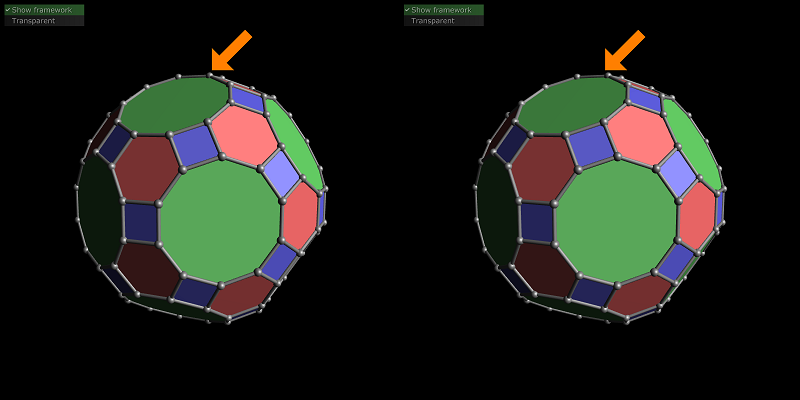
\includegraphics[scale=0.4]{bitmaps/stereosample.png}
\caption{A sample stereo rendering of a polyhedron with a cursor on top.}
\label{stereosample}
\end{figure}


\subsection{Polarisation stereo projection}
One of the principal aims of \softwarename\ is to work in conjunction with stereo projection systems that are based on polarisation. Such polarisation stereo projection systems (also sometimes called passive stereo) offer high quality immersive 3D projection at a low cost, and  typically consist in the following relatively items:
\begin{itemize}
\item A computer with a fast graphics card and dual screen output, running appropriate software (such as \softwarename).
\item Two data projectors that are connected to both screen outputs.
\item Two different polarising filters that are fitted in front of the projectors (e.g. 45� left and 45� right)
\item A non--depolarising projection screen (sometimes also called a silverscreen)
\item A number of polarised looking glasses.
\end{itemize}
See e.g. the GeoWall consortium (\url{http://www.geowall.org/} or \url{http://en.wikipedia.org/wiki/GeoWall}) for more information about how this kind of stereo visualisation systems work, and how to assemble such a system.

In order to configure \softwarename\ to work properly on such a system, it is crucial to realise that the left eye image should be sent to one projector, and the right eye image to the other. This can be achieved using the dual monitor feature of Windows, which creates a single virtual desktop that spans over both projectors. The \renderwin\ used \softwarename\ should then be configured in such a way that is exactly spans over the full desktop, and hence covers both screens. The left half of the \renderwin\ will then be sent to the left projector, and the right half to the right projector. Since, in stereo mode, \softwarename\ displays the left eye rendering and the right eye rendering side by side, the desired setup should be achieved.

You can setup the dimensions of the \renderwin in the settings scripts (see \ref{settings}). More specifically, \textbf{Display offset X} and \textbf{Display offset Y} specify the position of the top left corner of this window, in pixels, whereas \textbf{Display size X} and \textbf{Display size Y} specify the horizontal and vertical dimension of the \renderwin, also in pixels.

For example, suppose that two projectors are used with a resolution of $1024 \times 768$ pixels. The dual screen modus of Windows will create a single, virtual desktop that puts both projectors side by side, creating a total desktop resolution of $2048 \times 768$ pixels. In order to make \softwarename\ work correctly on such a system, the following values should be entered:

\begin{tabular}{l l}
\hline
Setting & Value \\ \hline
Show in stereo & checked \\
Swap left and right & \textit{dependent on the cabling of the projectors} \\
Display offset X & 0 \\
Display offset Y & 0 \\
Display size X & 2048 \\
Display size Y & 768 \\
\hline
\end{tabular}

\subsection{Parallel viewing and cross viewing}
A low budget way of viewing the animations in 3D is by simply looking at them side by side on a computer monitor, and try to make the stereo effect pop up. You can set up the image size that is optimal for this kind of viewing on your system by changing \textbf{Display Size X} and \textbf{Display Size Y}.

\subsection{Mirror viewing}
Another great way to see the animations in stereo is the usage of mirrors or prisms (see e.g. 
\url{http://nzphoto.tripod.com/sterea/stereomirror.htm}). To facilitate this kind of viewing, \softwarename\ offers complete freedom when it comes to flipping both stereo images. For both the left and right eye image, you can independently chose to mirror the image horizontally and/or vertically.

\subsection{The stereo baseline and stereo distance \label{stereobaseline}}
Two important parameters determine the way a scene is visualised in stereo:
\begin{description}
\item[Stereo distance] When a 3D scene is visualised as a stereo pair on a device (e.g. projected on a screen using polarisation projection), the viewer will see each component of the scene at a specific distance with respect to the screen. Some components will appear to float in front of the screen (hence this is often called immersive 3D), other components will appear to be at the same distance of the screen, and other components will appear behind the screen. Objects that appear at the same distance of the screen are said to have a zero parallax, because they have exactly the same position on both eye images. The stereo distance is the distance, measured in the 3D scene, from the viewer at which components of the scene are rendered with zero parallax.
\item[Stereo baseline] This is the distance between the left and right eye camera position in the scene. In many cases, it is meaningless to render a scene with a stereo baseline that is identical to the distance between the human eyes. For example, suppose that the animation shows the movement of the Planets around the Sun. A ``normal'' stereo baseline would show all planets at a distance of infinity, just like we see the stars in reality. Of course, in that case, the advantage of using a 3D rendering vanishes. Therefore, it is customary to use ``hyperstereo'', a technique where the stereo baseline is artificially boosted. The effect of hyperstereo can be interpreted in two ways:
\begin{enumerate}
\item A huge creature, with a large distance between both eyes, looks at the scene.
\item A normal human being (with standard eye separation) looks at a reduced scale model of the scene. The reduction factor is equal to the magnification factor of the stereo baseline.
\end{enumerate}
\end{description}
Most animations in \softwarename\ automatically control the stereo distance in a meaningful way, depending on the scene that is shown. In addition, the stereo baseline is automatically set as a constant fraction of the stereo distance, which ensures that a reasonable 3D effect is always visible. This fraction is determined by the \textbf{Eye separation factor} parameter in the settings.



\section{Warped rendering}
With\softwarename, it is possible to apply a two-dimensional distortion to the rendered image. This can be useful in a number of different situations, e.g.:
\begin{itemize}
\item Dome projection using a fisheye lens or a spherical mirror
\item Visualisation of 360-degree stereo pictures
\item Special projections, e.g. making a celestial chart
\end{itemize}

The definition of the warping can be specified in the init script. Below is an example of how this can be implemented:

\begin{lstlisting}
vp=addviewport(0,0,1,1,displayname,displayname);
...
warpx=matrix(101,101);
warpy=matrix(101,101);
for ix=0 to 100 do
   for iy=0 to 100 do {
      x=ix/100;
      y=iy/100;
      warpx(ix,iy)=x/(1+y);
      warpy(ix,iy)=y*(0.5+0.5*x);
   }
vp.EnableWarped(2000,1500,warpx,warpy);
\end{lstlisting}

%\chapter{Stereo rendering \label{stereorendering}}

\chapter{User interface}

\section{Introduction}

\important{
An animation script may disable and/or override the default UI actions. The following sections describe the default behaviour.
}

The software supports four different types of input devices: the keyboard, the mouse, a 3D mouse (SpaceNavigator or equivalent) or a gamepad (or joystick). Generally spoken, the user can interact with an animation in three possible ways:
\begin{description}
\item[Position.] The scene is viewed through a fictitious ``camera''. The user can change the position and direction of that camera.
\item[Time.] For animations that evolve over time (e.g. the movement of the Planets around the Sun), the script often applies an artificial time speedup factor in order to visuale phenomenons that would take too long to show up in real time. The user can change this time speedup factor, pauze the time evolution or even reverse the direction of time.
\item[UI Controls.] Some scripts display additional controls, such as check boxes, buttons or menu's. These controls can be used to change the behaviour of an animation.
\end{description}

\section{Keyboard shortcut keys}
Several important actions are only available through keyboard shortcuts. The following table gives an overview of the default keyboard shortcuts that are of general use in most scripts. Note that a specific script may override, disable or add specific keyboard shortcuts.

\begin{tabular}{ l p{1.5cm} p{11cm} }
\hline
Keyboard & Gamepad key nr. & Function
\\ \hline

F1 & 1 & Show or hide cursor 
\\
F2 & 2 & Show or hide user interface controls
\\
F3 & 3 & Pauze or resume the animation
\\
Shift+F3 & 8+3 & Reverse the time direction of the animation
\\
Enter & 5 & Execute a menu item, presses a UI button or changes the state of an UI checkbox
\\
Escape & 7 & Stop the animation
\\
Ctrl+Z & & Force the animation to stop (interrupt script)
\\
Ctrl+S & & Switch between mono and stereo view
\\
Ctrl+L & & Show or hide colored depth layers
\\
Ctrl+G & & Show or hide stereo align grid
\\
Ctrl+I & & Show or hide status line
\\
ctrl+P & & Copy the camera position to the clipboard
\\
ctrl+Shift+P & & Copy the cursor position to the clipboard
\\
ctrl+E & & Saves the current scene image to \filename{screendump.jpg} in the \datadir.
\\
\hline
\end{tabular}


\section{User navigation}

Navigating both in space and time is an important aspect of the interaction between the user and an animation. \softwarename\ uses the metaphor of a virtual camera through which the scene of the animation is seen. There is a variety of ways in which the user can control space and time through one or more of the input devices attached to the computer. To understand the logic behind this, two concepts are crucial: Axes and Modifiers. The activation of an Axis, accompanied by a Modifier, triggers a specific effect.

The following table gives a list of all available Axes, and how they can be activated using the keyboard, mouse or gamepad:

\begin{tabular}{l l l l}
\hline
Axis & Keyboard & Mouse & Gamepad \\ \hline
X & Arrow Left/Right & Move left/right  & Joystick 2 left/right \\
Y & Arrow Up/Down & Move up/down & Joystick 2 up/down \\
Z & Page Up/Down & Mouse wheel & Joystick 1 up/down\\
\hline
\end{tabular}

The following table gives a list of all modifiers, and how they can be activated on the keyboard, mouse or gamepad:

\begin{tabular}{l l l}
\hline
Modifier & Keyboard and Mouse & Gamepad \\ \hline
M0 & Press shift key & \textit{no extra button} \\
M1 & Press control key & Press button 6 \\
M2 & \textit{no extra key} & Press button 8 \\
\hline
\end{tabular}

Finally, the following table enumerates the effects of the activation of an axis, combined with a modifier:

\begin{tabular}{l l l l}
\hline
Modifier & Axis & Effect \\ \hline
M0 & X & Rotate camera horizontal \\
M0 & Y & Rotate camera vertical \\
M0 & Z & Move camera foward/back \\
M1 & X & Rotate scene horizontal \\
M1 & Y & Rotate scene vertical \\
M1 & Z & Zoom scene \\
M2 & X & No effect \\
M2 & Y & No effect \\
M2 & Z & Modify time speed  \\
\hline
\end{tabular}

NOTE: If the cursor is displayed (e.g. by pressing the F1 key), the M2 modifier combined with an axis moves the cursor over the scene (see \ref{thecursor}).

In order to further illustrate how the combination of an axis and a modifier gives a specific effect, the following list gives some examples:
\begin{itemize}
\item Rotate the camera to the right: press the Shift key + Right arrow (Shift triggers Modifier M0 and the Right arrow triggers the X axis). You can also press the Shift key while moving the mouse to the right. The same effect can be obtained by moving the Joystick 2 to the right on a gamepad.
\item Increase the time speed: press the Page Up key (triggering the Z axis; Modifier M2 corresponds to pressing no extra key on the keyboard). On the gamepad, you can move joystick 1 up while pressing button 8.
\end{itemize}

Note that, if present, \softwarename also supports the usage of a 3D mouse (SpaceNavigator), which provides the most powerful and flexible way of navigating through the 3D space.

\section{User interface controls}
Some scripts show special UI controls on top of the animation, allowing the user to control certain aspects of the animation. While the animation is running, the user can chose to hide or display these controls by pressing the F2 key (sometimes, it may be preferrable to have an uncluttered view on the scene by temporarily hiding these controls). When controls are displayed, there is always one control active, and surrounded by a green rectangle. The status of the active control can be modified by the user. Switching the active control can be done using the keyboard by pressing the TAB key, the Left/Right arrow keys. On the gamepad, the Left/Right buttons of the rocker pad have the same effect.

\begin{description}
\item[Editbox.] Used to enter text. When active, the user can type text using the keyboard, and erase with the Back key. 
\item[Valuebox.] Used to enter a numerical value. The control displays both the value and a graphic visualisation on a slider. When active, the value is modified using the Up/Down arrow keys.
\item[Checkbox.] Used to enter a boolean (yes/no) status. When active, pressing the Enter key changes the status.
\item[Listbox.] Used to pick a value from a list of choices. When active, using the Up and Down arrow keys changes the selection.
\item[Menu.] Used to present a menu with optional submenu's. The items are arranged vertically, and optional submenu's are displayed on the right of the parent item (with an arrow indicating that this item contains a submenu). When active, the Up/Down arrow keys navigate through a list of menu items at the same level, the Right arrow key enters a submenu (if any), and the Left arrow key jumps to the parent menu item of the current submenu (if applicable). Enter executes the selected menu item. Some menu items may have a checked/unchecked state.
\item[Button.] Represents an action button. When active, pressing the Enter key executes the associated action.
\end{description}

\section{The cursor \label{thecursor}}
In almost every animation, it is possible to show a cursor in order to point to specific aspects of the scene. This cursor is displayed as a yellow arrow. Pressing the F1 key (or button 1 on the gamepad) toggles the presence or absense of the cursor. When the cursor is active, it can be moved by the mouse (with the scroll wheel acting as the third dimension), or with the gamepad using joystick 2 while pressing button 8.


\chapter{Stereo pictures}

\softwarename\ comes with a number of pre--defined animations that make it a powerful software for browsing stereo pictures and for making beautiful slideshows of stereo pictures, using real 3D transition effects, sounds and text overlays.

Stereo pictures have to be in jpeg format, and the left and right eye picture should be stored side by side in a single image file, with the same resolution. The actual resolution (number of pixels) and the aspect ratio can be chosen freely for each picture, and does not have to correspond to the resolution and aspect ratio of the 3D display system. \softwarename\ will automatically rescale everything to the correct dimensions.

\important{Creating good-looking stereo pictures in an art by itself. Look on the web for recommendations on how to create proper stereo pictures, and for software that assists in this.}

\section{Stereo foto browser}

\begin{figure}
\includegraphics[width=120mm]{bitmaps/stereobrowser.jpg}
\caption{A screen view of the stereobrowser (in monoscopic representation).}
\label{stereobrowser}
\end{figure}


The script \animation{Stereo pictures \sep Browse Stereo pictures} can be used as a fancy browser for stereo pictures. On the proper hardware (see \ref{stereorendering} for more details), the stereo pictures as well as the thumbnails will be displayed in 3D.


\subsection{Setting up the browser}

Th script \animation{Stereo pictures \sep Stereo picture settings} can be used to set some basic properties of the stereo browser. The browser will automatically look for stereo foto content in subfolders of a specific \term{stereo pictures folder}. Default (if nothing is filled in), the subdirectory \filename{StereoPictures} of the \datadir\ is used, but you can specify any other folder on your system.

A second parameter is the number of rows that will be shown by the browser when the thumbnails are previewed. This number can range between 2 and 6.

Before using the browser, you should create stereo thumbnails for each stereo picture in your stereo picture folder. You can do this with the script \animation{Stereo pictures \sep Create Thumbnails}. When you launch this script, it will automatically scan all subdirectories of the current stereo picture folder, and create thumbnails for new pictures or for pictures that have been modified since the last thumbnail generation. Note that, for large sets of pictures, this may take a while.

\subsection{Using the browser}

When you launch the browser (\animation{Stereo pictures \sep Browse Stereo pictures}), it will first display a menu with all the subdirectories of the \term{stereo pictures folder} (subdirectories of subdirectories will appear as submenu items). You can select any folder and press Enter to start browsing through the thumbnails of the stereo pictures in this folder. To navigate through the thumbnails, you can use the arrow keys, or you can move the mouse.

At any time, there is an active picture that is highlighted and surrounded by an orange triangle. The active picture will automatically change if you navigate through the thumbnails. You can show the active picture in full screen by pressing the Enter key, or by clicking the left mouse button. In this full screen view, you can jump to the next or previous image with the Down and Up arrow keys, or return to the thumbnail overview by pressing Enter, Escape or by clicking the left mouse button. To exit the browser, press Escape while in thumbnail mode.

\section{Stereo photo slideshows}
\softwarename can be used to create fancy slideshows for stereo pictures that can be rendered in 3D, including 3D transition effects, sounds and text overlays. This functionality is provided in the pre--installed script \animation{Stereo pictures \sep Slide shows}.

A slide show is created by the user a as a very simple version of a \scriptlang script file (see chapter \ref{scriptdevelopment}). All slide show scripts should be placed in the subdirectory \filename{SlideShows} of the \datadir, and have the file extension \filename{.SCI}. Such a slide show script file contains all the directives to build up a show. When \animation{Stereo pictures \sep Slide shows} is launched, it will show a menu with an overview of all slide show scripts in the \filename{SlideShows} subdirectory. The user can pick one and press Enter to start it.

Below is the listing of a sample slide show script:

\begin{lstlisting}[numbers=left]
Picturefolder(datadir+"\StereoPictures\Sample set");
Transition("Curtain",2);
SoundFolder(datadir+"\sounds");

PlaySound("sound3.mp3",1000);
Delay(1);

ShowStereoPic("0001");
Delay(2);
ShowText("This is the first picture",point(-0.25,-0.2,0.1),
         "Size":0.05,"Color":color(1,0.7,0));
Delay(10);

ShowStereoPic("0002");
Delay(2);
ShowText("And this is the second",point(-0.25,-0.2,0.1),
         "Size":0.05,"Color":color(1,0.7,0));
Delay(10);

ShowStereoPic("0003");
Delay(10);

ShowStereoPic("0004");
Delay(10);

ShowStereoPic("0005");
FadeSound("sound3.mp3",0,10);
Delay(10);

end;
\end{lstlisting}

Lines 1--6 contain some initial setup. In line 1, the directory is specified where the stereo pictures are to be looked for. Note that \sourcecode{datadir} is a script function that automatically returns the \datadir\ (see \ref{F:DataDir}). In line 2, the current transition effect is specified and the duration of each transition. Line 3 sets the directory where sound files will be loaded from. Line 5 starts a music.

The remainder of the file describes the sequence of pictures. For example, line 8 shows the stereo picture \filename{0001}. Line 10 adds some text in overlay, and line 12 introduces a delay of 10 seconds. Line 27 fades out the music and line 30 ends the show.

\subsection{List of slide show commands}

\subsubsection{PictureFolder(Foldername)}
Sets the current location where the script will look for the stereo pictures. Note that you can repeat this command at any time in the slide show script to take pictures from a different location.

\subsubsection{VideoFolder(Foldername)}
Sets the current location where the script will look for the stereo videos. Note that you can repeat this command at any time in the slide show script to take videos from a different location.

\subsubsection{Transition(Type, Delay)}
Specifies the current transition type and duration of the transition (in seconds). Current transitions effects include the following options:
\begin{description}
\item[Fade] fades previous to black and then fades next in
\item[Curtain] applies a 3D curtain--like effect to move prevous out and next in
\item[Transient] cross-fades previous and next simultaneously
\item[Zoom] Zoom and fade out of previous, and zoom and fade in of next
\end{description}

\subsubsection{ShowStereoPic(Imagename, \textit{optional extra arguments})}
Shows a new stereo picture. The extra arguments can take the form of
\begin{description}
\item["Size":value] specifies the size of the picture on the screen (``1'' is full--screen).
\item["Position":point(x,y,z)] specifies the 3D position where the picture should be shown. Default is $(0,0,0)$. The $Z$--dimension corresponds to the distance from the viewer.
\end{description}
Note that you can show more than one stereo picture simultaneously. You can use the optional Size and Position arguments to arrange several pictures on the screen.

\subsubsection{HideStereoPic(Imagename)}
Removes a visible stereo picture.

\subsubsection{panstereopic(imagename, \textit{optional extra arguments}))}
Pans a stereo picture to a new position. The extra arguments can take the form of
\begin{description}
\item["Duration":value] specifies the duration of the panning action in seconds.
\item["Position":point(x,y,z)] specifies the new target 3D position where the picture should be panned to.
\end{description}

\subsubsection{AutoHidePrevious(NewStatus)}
Determines whether or not the previous picture will automatically be removed when the next is shown. \sourcecode{NewStatus} can be \sourcecode{True} or \sourcecode{False}. (default is \sourcecode{True}).

\subsubsection{showstereovideo(filename)}
Plays a stereo video.


\subsubsection{ShowText(Content, Position, \textit{optional extra arguments})}
Shows the string \sourcecode{Content} on top of the current picture, at the specified position (provided as \sourcecode{Point(x,y,z)}. Optional arguments include:
\begin{description}
\item["Size":value] specifies the size of the text.
\item["Color":Color(r,g,b)] specifies the color of the text, using the Red (r), Green (g) and Blue (b) values, each one ranging between $0$ and $1$.
\end{description}

\subsubsection{SoundFolder(Foldername)}
Sets the current location where script will look for the sound files. Note that you can repeat this command at any time in the slide show script to take sound files from a different location.

\subsubsection{PlaySound(Filename, Volume)}
Plays a sound file at a specific volume

\subsubsection{StopSound(Filename)}
Stops the playing of a sound file.

\subsubsection{FadeSound(Filename, NewVolume, Duration)}
Fades in or out a playing sound file to a new volume, over a specific period of time (in seconds).

\subsubsection{Delay(Duration)}
Tells the script to wait for a specified number of seconds.

\subsubsection{End}
Indicates the end of the show. \softwarename\ will return to the start menu.

\subsubsection{Loop}
Indicates that the show should continue from the top of the script. This can be used to create slide shows that run in an auto repeat mode.


\chapter{Script development \label{scriptdevelopment}}

\section{Introduction}

\important{
This chapter is not intended to be a complete tutorial on how to develop scripts in \softwarename, the only purpose is to provide a getting started. The best way of getting familiar with the script development is to study the pre--defined scripts that come with the software. Nevertheless, anyone who intends to start developing for \softwarename, should have a good knowledge of programming in another (script) language.
}

To start the development environment, you first need to make sure that no script is currently running in the software. This can be achieved by pressing Ctrl+Z repeatedly until the last script stops (note that the startup screen with the menu overview of all animations is a script by itself). You can then bring the \sourcewin\ to the top of the window stack using the Windows Alt+TAB keyboard combination.

\section{The source code window}
\begin{figure}
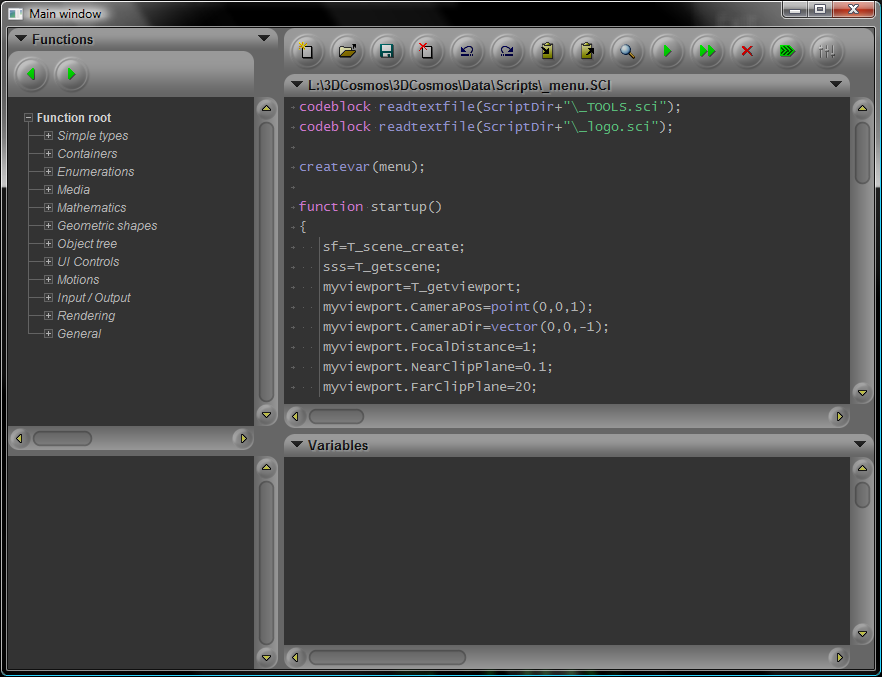
\includegraphics[scale=0.4]{bitmaps/sourcecodewindow.png}
\caption{The source code window.}
\label{sourcecodewindow}
\end{figure}
When the \sourcewin\ is opened (see \figref{sourcecodewindow}), it is divided in three different parts:
\begin{itemize}
\item On the left side, over the full height, the \functionspanel\ is shown. Underneath this panel, the \objectspanel\ is hidden. You can switch between both panel by clicking on the header, and chosing the appropriate panel name from the context menu.
\item On the top right side is the \sourcecodepanel.
\item On the bottom right side is the \varspanel. Underneath this panel, the \outputpanel\ is hidden. You can switch between both panel by clicking on the header, and chosing the appropriate panel name from the context menu.
\end{itemize}

\subsection{The \sourcecodepanel}
This panel displays the source code of the active script. The file name of the script is displayed in the header of the panel. If several scripts are loaded simultaneously, you can switch between them by clicking on the header (where the file name is displayed), and selecting another script from the context menu. The two arrows pointing down at the edges of the header indicate that more options are available at this panel, hidden behind the current view. Table \ref{sourcecodewindowcommand} gives an overview of all the commands that are available in the source code \sourcecodepanel. In addition, the script editor accepts most standard Windows keyboard shortcuts, such as Ctrl+C for Copy, Ctrl+V for paste, etc...

\begin{table}
\begin{tabular}{l p{12cm} }
\hline
Button & Description \\ \hline
BT1 & Create a new script \\
BT2 & Open an existing script \\
BT3 & Save the active script \\
BT4 & Close the active script (removing it from the \sourcecodepanel, but keeping the version on disk) \\
BT5 & Undo the last edit action \\
BT6 & Redo the last action that was undone \\
BT7 & Copy the current selection to the clipboard \\
BT8 & Paste the content of the clipboard \\
BT9 & Search for text in the active script \\
BT10 & Start the debugging of the active scipt \\
BT11 & Run the acrtiv script in debug mode \\
BT12 & Stop the execution of the script \\
BT13 & Animate the active script \\
BT14 & Open the settings dialog box \\
\hline
\end{tabular}
\caption{Commands of the code window.}
\label{sourcecodewindowcommand}
\end{table}


\subsection{The \functionspanel}
In order to assist the exploration of the rich programming environment offered by \scriptlang, this panel offers an overview of all available classes and functions, logically arranged into a tree. You can expand and collapse branches in the tree by clicking on the boxes. For each component of the function tree, the lower part of the panel gives a brief description of its functionality. This description may have hyperlinks that lead to other parts of the function tree. You can copy a specific funcion or class name into the source code by pressing the Ctrl key while clicking on the name in the tree.

\subsection{The \varspanel}
If a script is running in debug mode, this panel displays a list of all existing variables, with their content.

\subsection{The \outputpanel}
As a part of a debugging process, a script may write information to this panel using the script function \filename{output}.

\subsection{The \objectspanel}
The current state of \softwarename, including the scene(s), subframes, geometric objects that appear in these scenes, motions, textures, etc... are all maintained in a single tree structure called the \objecttree. This is a very important concept in the software, because it provides a complete description of the current state of the animation. At any time, the \objectspanel\ gives an overview of this \objecttree. In the lower part of this panel, the properties of the selected object in the tree are displayed. This panel can be used as a debugging tool to get better insight in the current state of the software.

\section{Fundamentals of \scriptlang}

\subsection{Types and variables}
\scriptlang\ shares many properties with modern script languages, such as JavaScript. Statements are separated by semicolons (\sourcecode{;}). The language is structured and object--oriented, and uses dynamic typing. This means that data types (\sourcecode{string}, \sourcecode{scalar}, \sourcecode{time}, ...) are associated with \emph{values}, and not with \emph{variables}. In addition, variables do not have to be declared explicity, since their existence is triggered by an assignment operation. For example:

\begin{lstlisting}
x="abc";
x=42;
x=time(2010,1,1,0,0,0);
\end{lstlisting}

consecutively assigns to the variable \sourcecode{x} the string "`abc"', the value 42, and a time corresponding to January 1 2010, 0h UT.

Apart from explicity assignment of a variable to a value, there are two other ways to create a variable. One is the assignment to a data type. For example, \sourcecode{mylist=list;} creates a new variable with name ``mylist'' that holds a list object. Another method is to use the function \sourcecode{createvar}, which creates a variable that is not assigned to any data content.

\important{
In \scriptlang, there is no distinction between the conventional ``float'' and ``integer'' data types: both are \sourcecode{scalar} (\ref{T:Scalar}) object types. An integer is simply a \sourcecode{scalar} with an integral value.
}

\scriptlang contains a large number of object types, that can roughly be categorized in three classes: basic object types, container object types and animation object types. A complete description of all object types is beyond the scope of this section, but the \functionspanel\ in the \sourcewin\ offers a great starting point to start exploring all available object types.

\subsection{Basic object types}
Object types that fall in this category are not necessarily simple by nature, but distinguish themselves from animation object types because they have a general meaning that makes sense outside the scope of \softwarename. The ``Simple types'' branch (\ref{Simple types}) contains conventional object types such as \sourcecode{string} (\ref{T:String}), \sourcecode{scalar} (\ref{T:Scalar}) and \sourcecode{time} (\ref{T:Time}) are present.

In addition, \scriptlang\ also knows a large amount of specific data types that can be used to perform mathematical manipulations with 3D geometry, available under the ``Mathematics'' (\ref{Mathematics}) branch of the \functionspanel. For example, there are \sourcecode{point} (\ref{T:Point}) and \sourcecode{vector} (\ref{T:Vector}) object types, but also more sophisticated concepts are available, such as the \sourcecode{LineSegment} (\ref{T:LineSegment}) and \sourcecode{Transformation} (\ref{T:Transformation}) object types.

In addition, the ``Media'' branch (\ref{Media}) of the \functionspanel\ offers a number of object types that are associated with multimedia: \sourcecode{Bitmap} (\ref{T:Bitmap}), \sourcecode{Video} (\ref{T:Video}) and \sourcecode{Sound} (\ref{T:Sound}).

\subsection{Container object types}
There are object types that serve as a container to group several objects into a single new object.
\subsubsection{List (\ref{T:List})}
A list is linear collection of objects, accessible through an index (i.e. a \sourcecode{scalar} with an integral value). Note that these components do not have to have the same object type. Individual components in a list object are addressable with the \sourcecode{()} operator:

\begin{lstlisting}
mylist(0)="abc";
mylist(1)="def";
mylist(2)=42;
mylist(10)=point(0,0,0);
result=mylist(10);
\end{lstlisting}

\subsubsection{Map (\ref{T:Map})}
A map is a collection of objects, each one identified by a unique string. As a syntax shortcut, the dot operator can be used to address the components of a map, creating a class--like syntax:

\begin{lstlisting}
mymap=map;
mp.myname="This is my name";
mp.myval=42;
mp.mypoint=point(1,2,3);
\end{lstlisting}

\subsection{Animation object types}
Under the ``Object Tree'' branch (\ref{Object tree}) of the \functionspanel, a large number of objects types is available that are used as building blocks for scenes in animations. This includes object types like \sourcecode{Subframe} (\ref{T:Subframe}), \sourcecode{Sphere} (\ref{T:Sphere}), \sourcecode{Cylinder} (\ref{T:Cylinder}), etc... Objects that belong to one of these types will automatically become member of the current \objecttree\ of \softwarename, and appear in the \objectspanel.

\subsection{Custom functions}
You can declare a custom function in \scriptlang with the \sourcecode{function} statement:

\begin{lstlisting}
function myfunction(arg1,arg2)
{
   return(arg1+arg2);
}
\end{lstlisting}

Note that \scriptlang\ is very relax in the way a custom function is declared: the object type of the argument(s) and return value is not specified. Only at run--time will the variables \sourcecode{arg1} and sourcecode{arg2} have a specific type. If the $+$ operator is defined for these types, the function will successfully return the result. If not, a run--time error will be generated.


\subsection{Including code from other locations}
You can dynamically insert code at a specific point in the script using the \sourcecode{codeblock} directive. This directive should be followed by a string or an expression that evaluates to a string. A typical example is the inclusion of the source code from another script file:

%\lstset{numbers=left, numberstyle=\tiny, stepnumber=1, numbersep=5pt}

\begin{lstlisting}
codeblock readtextfile(ScriptDir+"\_TOOLS.sci");
\end{lstlisting}

The function \sourcecode{readtextfile} (\ref{F:readtextfile}) takes a file name and returns the content of that file as a string, which is in turn inserted as code at this point by the \sourcecode{codeblock} directive.

\section{A sample animation script}

The following \scriptlang script implements a simple but operational animation, showing a rotating bar. It can be found as \filename{sample.sci} in the pre--installed set of scripts.

\begin{lstlisting}[numbers=left]
codeblock readtextfile(ScriptDir+"\_TOOLS.sci");

rootframe=T_scene_create;
root.SC.AmbientLightColor=color(0.2,0.2,0.2);

vp=T_getviewport;
vp.CameraPos=point(0,5,10);
vp.CameraDir=vecnorm(point(0,0,0)-vp.camerapos);
vp.FocalDistance=10;
vp.NearClipPlane=0.1;
vp.FarClipPlane=20;

mybarframe=rootframe.addsubframe("BarFrame");
rotation=MotionRotate.create(mybarframe,"MyRotation");
rotation.NormDir=vector(0,1,0);
mybarframe.MotionName=rotation.name;
mybar=mybarframe.add("bar");
mybar.SizeX=2;mybar.SizeY=1;mybar.SizeZ=0.5;
mybar.position=point(-1,-0.5,-0.25);
mybar.color=color(0.3,0.9,0.5);

root.time=time(2010,1,1,0,0,0);
root.timespeedfactor=1;

while true do {
   incrtime;
   render;
}
\end{lstlisting}

This script can be used as an example for how a typical script is set up. There are always two major components:
\begin{description}
\item[The setup part.] The scene is initialised and al the components of the animation are created (lines 1--23).
\item[The animation loop.] The actual rendering and animation of the scene is performed in a loop (lines 25--28). In this case, the animation loop is as simple as it can get. In general, a lot of sophistication can be put in this loop in the form of script source code.
\end{description}

Line 1 tells compiler to include the source code that is found in the script \filename{\_TOOLS.SCI} in the standard scripts directory (this is the ``Scripts'' subdirectory of the \datadir). This script contains a number of utilities that are used in almost every script.

Line 3 calls the function \sourcecode{T\_scene\_create}, which can be found in \filename{\_TOOLS.SCI}, and performes a complete initialisation of a new scene (\ref{T:Scene}), returning the default subframe (\ref{T:Subframe}) of this scene.

Line 4 sets the ambient color of the new scene (\ref{F:Scene:AmbientLightColor}).

Line 6 calls the function \sourcecode{T\_getviewport} (also present in \filename{\_TOOLS.SCI}), which returns the viewport (\ref{T:Viewport}) that was created by \sourcecode{T\_scene\_create}. This viewport is stored in the variable \sourcecode{vp}.

Line 7 sets the position of the fictitious camera that is used to record the scene (\ref{F:Viewport:CameraPos}).

Line 8 sets the viewing direction of this camera. Using elementary vector calculation, it is set in such a way that it looks at the origin (\ref{F:Viewport:CameraDir}).

Line 9 sets the ``focal distance'' or stereo baseline (see \ref{stereobaseline}) (\ref{F:Viewport:FocalDistance}).

Line 10 and 11 set the front and back clipping distances for the rendering of the scene. Anything that is closer to the camera than \sourcecode{NearClipPlane} (\ref{F:Viewport:NearClipPlane}) or further away than \sourcecode{FarClipPlane} (\ref{F:Viewport:FarClipPlane}), will not be rendered.

Line 13 creates a new subframe (\ref{T:Subframe}), that will hold the bar object and will have a motion attached to it.

Line 14 defines a rotation--style motion (\ref{T:MotionRotate}). The ``Motions'' branch (\ref{Motions})contains a list of all possible motions. Line 15 sets the rotation axis equal to the Y--axis.

Line 16 Specifies that the subframe ``BarFrame'' should be animated according to this motion (\ref{F:Subframe:MotionName}).

Line 17 Creates a bar object in the subframe (\ref{F:Subframe:add}, \ref{T:Bar}). Lines 18--20 specify the color, dimensions and position of this bar. Because this bar was created in the subframe ``BarFrame'', it will automatically follow the motion attached to this subframe.

Line 22 and 23 specify the start time of the animation (\ref{F:ObjectRoot:Time}) and the animation time multiplication factor (\ref{F:ObjectRoot:TimeSpeedFactor}). In this case, the animation runs in real time.
Line 25--28 are the animation loop. Each cycle of the loop consists in two steps: increasing the time (\sourcecode{incrtime}, \ref{F:incrtime}) and rendering the scene to the \renderwin\ (\sourcecode{render}, \ref{F:render}).

\section{The Object Tree}
The \objecttree\ is a crucial concept in writing animations for \softwarename. During the setup phase of the animation, this tree will be populated with important elements such as a scene, the viewport, subframes, geometrical objects, motions, textures, etc... Most of the required elements (the root, a single scene with a single subframe and a single viewport) are set up automatically by the helper function \sourcecode{T\_scene\_create} in \filename{\_TOOLS.SCI}.

\subsection{The Object Root}
There is always a single \term{Object Root} (\ref{T:ObjectRoot}) present. It contains a number of important properties, most of which are set automatically by the pre--defined Setup script (\ref{settings}). In addition, it also contains a number of properties that must be set by the animation, such as the current time and the time speed factor.

\subsection{Viewports}
In most animations, the \term{Object Root} will contain exactly one \term{Viewport} (\ref{T:Viewport}). A \term{viewport} contains all the information about how the scene is registered by the virtual camera for rendering to the \renderwin: the camera position, orientation and aperture, the stereo settings, the front and back clipping planes, etc... Many properties of the \term{viewport} are set by the global Settings script (\ref{settings}), but there are several important properties that need to be set by the animation script.

\subsection{Scenes}
In most animations, the \term{Object Root} will contain exactly one \term{Scene} (\ref{T:Scene}). A \term{scene} contains a number of important properties, such as the position and color of the light source(s), the background color, etc...

\subsection{Subframes}
Positions in the 3D world of a \term{scene} are defined by three coordinates $(x,y,z)$ in a orthonormal basis. When a more complex scene is built, it is often useful to define a part of it in a different basis. For example, suppose that the scene contains a car with four wheels. It is convenient to define a wheel relative to its center (preferably in a separate function), and specify where on the global scene this will should be positioned (both origin and direction). You can do this by defining a \term{subframe} (\ref{T:Subframe}), specify the basis of the coordinate system for this subframe in terms of the coordinate system of the global scene, and define the geometric objects that describe the wheel relative to this subframe. Repositioning of this wheel to a different position and/or direction on the scene then simply becomes a matter of manipulating the basis of this \term{subframe}. This can be done by accessing the property \sourcecode{Transf} (\ref{F:Subframe:Transf}), which sets or returns a \sourcecode{Transformation} object (\ref{T:Transformation}). Each scene should have at least one subframe.

\important{\softwarename\ uses homogeneous coordinates and affine transformations to describe the 3D space of a scene. A good understanding of these concepts and geometry in general is necessary to successfully write scripts that create scenes and animations.}

A \term{subframe} can belong to the \term{scene}, but it can also belong to another \term{subframe}. In this case, the basis of the new subframe is described relative to the basis of the parent subframe. In such a way, complex scenes can be described as hierarchical structures of nested \term{subframes}.

\subsection{Geometric objects}
The visible objects that build the scene are called \term{geometric objects}, and can be found in the \term{Object tree>Geometric Objects} branch of the \functionspanel. These objects can be added to a \term{subframe} using the member function \sourcecode{add} (\ref{F:Subframe:add}). Examples of such objects include spheres (\ref{T:Sphere}), cylinders (\ref{T:Cylinder}), but also text (\ref{T:Text3D}). These objects have numerous properties to define their appearance: visibility, color, texture...

\subsection{Textures}
A very powerful concept in 3D rendering are the so--called \term{textures}. This is a bitmap image that is wrapped over a geometric object, in order to give it a more realistic appearance. For example, a convincing rendering of the Earth as a planet can be created by wrapping a bitmap with a World map over a (flattened) sphere. A texture object in \softwarename\ (\ref{T:Texture}) is always member of a \term{subframe}, and can be created with the member function \sourcecode{CreateTexture} (\ref{F:Subframe:CreateTexture}). Once created, this texture can be assigned to an individual geometric object with the property \sourcecode{Texture} (e.g. \ref{F:Sphere:Texture} for Sphere objects). 

\subsection{Motions}
Many animations show moving objects. Usually, this is achieved by placing a moving object in a \term{subframe}, and change the move the basis that define this subframe with respect to its parent. There are two different approaches to achieve this:
\begin{enumerate}
\item In the render loop, calculate and set the new position of the subframe each time before rendering a new frame.
\item In the setup phase, define a \term{motion} that controls how the subframe is moving during the animation, and attach this motion to the corresponding subframe.
\end{enumerate}
The second option has the advantage that the source code of the script is usually simpler and easier to understand, and that the rendering may be faster because the pre--defined motions are optimised for calculation speed. The first option offers maximum flexibility, but is often harder to program. The ``Motions'' branch in the \functionspanel enumerates a list of all possible motions (see also \ref{Motions}).

Note that a motion can not only control the position of a \term{subframe} (i.e. the origin of its basis), but also its complete 3D orientation (i.e. the orientation of its orthogonal basis with respect to the parent subframe). A \term{motion} can apply a general \term{affine transformation} to the subframe (\ref{T:Transformation}). For example, a \sourcecode{MotionRotate}) object (\ref{T:MotionRotate}) causes a subframe to spin around a given axis, at a specific rotation speed.

\documentclass[10pt]{book}
\usepackage{hyperref}
\hypersetup{colorlinks=true,linkcolor=blue}
\newcommand{\linkitem}[1]{\hyperref[#1]{\nameref{#1} (\ref{#1})}}
\newcommand{\sourcecode}[1]{\texttt{#1}}
\newcommand{\var}[1]{\textit{#1}}
\newcommand{\softwarename}{Z--Flux}
\begin{document}
\chapter{Script language definition}
\section{Function root \label{}}
No description

\section{Simple types \label{Simple types}}

Data types that encapsulate geometric objects such as points and vectors can be found in \linkitem{Mathematics}.

\subsection{Type Anytype \label{T:Anytype}}
This is a generic object type that can stand for any specific object type.

\subsection{Type String \label{T:String}}
A String object type encapsulates a text string.

\subsubsection{String.Length \label{F:String:Length}}
Scalar X . \textbf{Length} \\
Returns the number of characters in a string.

\subsubsection{String.get \label{F:String:get}}
String X . \textbf{get} ( Scalar \textit{position} ) \\
Returns a single character from a string.

\subsubsection{String.substring \label{F:String:substring}}
String X . \textbf{substring} ( Scalar \textit{start}, Scalar \textit{stop} ) \\
Returns a part of a string, between the positions \var{start} and \var{stop}. Both values are zero-based. For example, the script \\
\sourcecode{
st="abcdef"; \\
st2=st.substring(2,3);
} \\
returns "cd" in \sourcecode{st2}.

\subsubsection{String.find \label{F:String:find}}
Scalar X . \textbf{find} ( String \textit{target} ) \\
Determines the position of the first occurrence of a subtring \var{target} in a string. This number is zero-based. If this substring does not occur, $-1$ is returned.

\subsubsection{String.split \label{F:String:split}}
String X . \textbf{split} ( String \textit{split} ) \\
Splits a string at the first occurrence of the string \var{split}. The left part is returned by the function, the right part is stored in the parent object of this function. For example, \\
\sourcecode{
st="abc-def"; \\
st2=st.split("-"); \\
}
Returns "def" in \sourcecode{st} and "abc" in \sourcecode{st2}.

\subsubsection{String.Replace \label{F:String:Replace}}
X . \textbf{Replace} ( String \textit{source}, String \textit{dest} ) \\
Replaces all occurrences of the string \var{source} by the string \var{dest}.
For example, \\
\sourcecode{
st="This is a test"; \\
st.Replace(" ","--"); \\
}
Returns "This--is--a--test" in \sourcecode{st}.


\subsubsection{String.Invert \label{F:String:Invert}}
X . \textbf{Invert} \\
Inverts the ordering of the characters in a string.

\subsubsection{Function Str \label{F:Str}}
String \textbf{Str} ( Anytype \textit{value} ) \\
Converts any data type to a string.

\subsubsection{Function Translate \label{F:Translate}}
String \textbf{Translate} ( String \textit{source} ) \\
Translates a string into the currently active language, using the language mapping files.

\subsubsection{Operator String + String \label{O:String+String}}
Concatenates two strings.

\subsubsection{Operator String $<$ String \label{O:String<String}}
Determines if the first string is lexicographically smaller than the second. This comparison is case insensitive.

\subsubsection{Operator String $<$= String \label{O:String<=String}}
Determines if the first string is lexicographically smaller than or equal to the second. This comparison is case insensitive.

\subsubsection{Operator String $>$ String \label{O:String>String}}
Determines if the first string is lexicographically larger than the second. This comparison is case insensitive.

\subsubsection{Operator String $>$= String \label{O:String>=String}}
Determines if the first string is lexicographically larger than or equal to the second. This comparison is case insensitive.

\subsubsection{Operator String == String \label{O:String==String}}
Determines if the first string equal to the second string. This comparison is case insensitive.

\subsubsection{Operator String != String \label{O:String!=String}}
Determines if the first string differs from the second string. This comparison is case insensitive.

\subsection{Type Scalar \label{T:Scalar}}
A scalar object type encapsulates a number. This number can be integral or floating point.

\subsubsection{Function ToScalar \label{F:ToScalar}}
Scalar \textbf{ToScalar} ( String \textit{value} ) \\
Converts a string to a scalar value.

\subsubsection{Function ScalarToString \label{F:ScalarToString}}
String \textbf{ScalarToString} ( Scalar \textit{value}, Scalar \textit{length}, Scalar \textit{digits} ) \\
Converts a scalar value to a string, where the total length of the string can be speficied, as well as the number of decimal positions. If necessary, the string is padded on the left with spaces.

\subsubsection{Function Min \label{F:Min}}
Scalar \textbf{Min} ( Scalar \textit{val1}, Scalar \textit{val2} ) \\
No description

\subsubsection{Function Max \label{F:Max}}
Scalar \textbf{Max} ( Scalar \textit{val1}, Scalar \textit{val2} ) \\
No description

\subsubsection{Operator Scalar + Scalar \label{O:Scalar+Scalar}}
Calculates the sum of two scalar values.

\subsubsection{Operator Scalar - Scalar \label{O:Scalar-Scalar}}
Calculates the difference between two scalar values.

\subsubsection{Operator Scalar * Scalar \label{O:Scalar*Scalar}}
Calculates the product of two scalar values.

\subsubsection{Operator Scalar / Scalar \label{O:Scalar/Scalar}}
Calculates the division of two scalar values.

\subsubsection{Operator Scalar $\wedge$ Scalar \label{O:Scalar^Scalar}}
Calculates the power of two scalar values.

\subsubsection{Operator Scalar $<$ Scalar \label{O:Scalar<Scalar}}
Determines if the first scalar value is smaller than the second.

\subsubsection{Operator Scalar $<$= Scalar \label{O:Scalar<=Scalar}}
Determines if the first scalar value is smaller than or equal to the second.

\subsubsection{Operator Scalar $>$ Scalar \label{O:Scalar>Scalar}}
Determines if the first scalar value is larger than the second.

\subsubsection{Operator Scalar $>$= Scalar \label{O:Scalar>=Scalar}}
Determines if the first scalar value is larger than or equal to the second.

\subsubsection{Operator Scalar == Scalar \label{O:Scalar==Scalar}}
Determines if two scalar values are equal.

\subsubsection{Operator Scalar != Scalar \label{O:Scalar!=Scalar}}
Determines if two scalar values are different.

\subsection{Type Bool \label{T:Bool}}
A Bool object type contains a boolean logical state, which can be True or False.

\subsubsection{Function not \label{F:not}}
Bool \textbf{not} ( Bool \textit{arg} )= \\
Inverts the value of a logical Bool value.

\subsubsection{Operator Bool  and  Bool \label{O:Bool and Bool}}
Applies the boolean AND operator on two boolean values.

\subsubsection{Operator Bool  or  Bool \label{O:Bool or Bool}}
Applies the boolean OR operator on two boolean values.

\subsection{Type Time \label{T:Time}}
A Time object variable encapsulates time information, including both a calendar date and a time of the day.

\subsubsection{Time.JD \label{F:Time:JD}}
Scalar X . \textbf{JD} = \\
Returns or sets the Julian date of a time object.

\subsubsection{Time.Year \label{F:Time:Year}}
Scalar X . \textbf{Year} = \\
Returns or sets the year value of a time object.

\subsubsection{Time.Month \label{F:Time:Month}}
Scalar X . \textbf{Month} = \\
Returns or sets the month value of a time object.

\subsubsection{Time.Day \label{F:Time:Day}}
Scalar X . \textbf{Day} = \\
Returns or sets the day value of a time object.


\subsubsection{Time.Hour \label{F:Time:Hour}}
Scalar X . \textbf{Hour} = \\
Returns or sets the hours value of a time object.


\subsubsection{Time.Min \label{F:Time:Min}}
Scalar X . \textbf{Min} = \\
Returns or sets the minutes value of a time object.


\subsubsection{Time.Sec \label{F:Time:Sec}}
Scalar X . \textbf{Sec} = \\
Returns or sets the seconds value of a time object.


\subsubsection{Time.AddSeconds \label{F:Time:AddSeconds}}
X . \textbf{AddSeconds} ( Scalar \textit{seconds} ) \\
Adds a number of seconds to a time object. This value can be positive and negative.

\subsubsection{Time.AddDays \label{F:Time:AddDays}}
X . \textbf{AddDays} ( Scalar \textit{days} ) \\
Adds a number of days to a time object. This value can be positive and negative.

\subsubsection{Time.DiffDays \label{F:Time:DiffDays}}
Scalar X . \textbf{DiffDays} ( Time \textit{reftime} ) \\
Calculates the time difference in seconds between the parent time object and the time object provided in \var{reftime}.

\subsubsection{Time.DiffSecs \label{F:Time:DiffSecs}}
Scalar X . \textbf{DiffSecs} ( Time \textit{reftime} ) \\
Calculates the time difference in days between the parent time object and the time object provided in \var{reftime}.


\subsubsection{Function time \label{F:time}}
Time \textbf{time} (  [ Scalar \textit{year}, Scalar \textit{month}, Scalar \textit{day}, Scalar \textit{hour}, Scalar \textit{min}, Scalar \textit{sec} ] ) \\
Constructs a time object, providing the calendar time and the time of the day.

\subsubsection{Function timeJD \label{F:timeJD}}
Time \textbf{timeJD} (  [ Scalar \textit{JD} ] ) \\
Returns a time object that corresponds to a Julian date provided in \var{JD}.

\subsubsection{Function CurrentTimeUT \label{F:CurrentTimeUT}}
Time \textbf{CurrentTimeUT} \\
Returns a time object that contains the current time in UT.

\subsubsection{Operator Time - Time \label{O:Time-Time}}
Subtracts two times from each other, and returns the difference in seconds.

\subsubsection{Operator Time + Scalar \label{O:Time+Scalar}}
Adds a number of seconds to a time value.

\subsubsection{Operator Time - Scalar \label{O:Time-Scalar}}
Subtracts a number of seconds from a time variable.

\subsection{Type Chrono \label{T:Chrono}}
Implements a chronometer object that can be used to measure time lapses.

\subsubsection{Chrono.Start \label{F:Chrono:Start}}
X . \textbf{Start} \\
Resets and starts the chronometer.

\subsubsection{Chrono.Pauze \label{F:Chrono:Pauze}}
X . \textbf{Pauze} \\
Pauzed the chronometer (the counting is suspended).

\subsubsection{Chrono.Resume \label{F:Chrono:Resume}}
X . \textbf{Resume} \\
Resumes the counting of the chronometer.

\subsubsection{Chrono.Set \label{F:Chrono:Set}}
X . \textbf{Set} ( Scalar \textit{time} ) \\
Sets the counter of the chronometer at a certain time (in seconds).

\subsubsection{Chrono.Elapsed \label{F:Chrono:Elapsed}}
Scalar X . \textbf{Elapsed} \\
Returns the elapsed number of seconds.

\subsection{Type Color \label{T:Color}}
A Color object type encapsulates color information, containing Red, Green, Bue and Transparancy values.

\subsubsection{Color.r \label{F:Color:r}}
Scalar X . \textbf{r} = \\
Returns or sets the red component of a Color object, ranging between $0$ and $1$.

\subsubsection{Color.g \label{F:Color:g}}
Scalar X . \textbf{g} = \\
Returns or sets the green component of a Color object, ranging between $0$ and $1$.


\subsubsection{Color.b \label{F:Color:b}}
Scalar X . \textbf{b} = \\
Returns or sets the blue component of a Color object, ranging between $0$ and $1$.


\subsubsection{Color.a \label{F:Color:a}}
Scalar X . \textbf{a} = \\
Returns or sets the transparency component of a Color object, ranging between $0$ and $1$.


\subsubsection{Function color \label{F:color}}
Color \textbf{color} ( Scalar \textit{r}, Scalar \textit{g}, Scalar \textit{b},  [ Scalar \textit{a} ] ) \\
Creates and returns a color object type, based on RGB values.

\subsubsection{Operator Color + Color \label{O:Color+Color}}
This operator can be used in conjunction with \linkitem{O:Scalar*Color} to calculate weighted averages between two or more colors.
For example, in the script: \\
\sourcecode{
col1=Color(1,0.5,0.25); \\
col2=Color(0,0.75,0.5); \\
colrs=2*col1+col2; \\
}
will \sourcecode{colrs} contain a color that is a weighted combination of \sourcecode{col1} and \sourcecode{col2}, where the former will be weighted twice as much as the latter.

\subsubsection{Operator Scalar * Color \label{O:Scalar*Color}}
See \linkitem{O:Color+Color} for more information.

\section{Containers \label{Containers}}
This section contains a number of data type that can be used to create compound objects, grouping several objects together in a structured way.

\subsection{Type List \label{T:List}}
A list implements an array of objects, addressed by an index number. Note that a list can contain any type of objects, in a mixed manner. For example, a list can contain other lists. List indices are zero-based.

Apart from the member functions that access the content of this list, you can also use an indexing operator, both for setting or returning an item of the list: \\
\sourcecode{
lst=list; \\
lst(0)="abc"; \\
lst(1)="def"; \\
lst(10)=12.7; \\
result=lst(10);
} \\

\subsubsection{List.clear \label{F:List:clear}}
X . \textbf{clear} \\
Resets a list to empty, clearing its content.

\subsubsection{List.size \label{F:List:size}}
Scalar X . \textbf{size} \\
Returns the number of items in a list.

\subsubsection{List.add \label{F:List:add}}
X . \textbf{add} ( Anytype \textit{comp} ) \\
Adds a new item to a list, appending it at the end of the list.

\subsubsection{List.get \label{F:List:get}}
Anytype X . \textbf{get} ( Scalar \textit{index} ) = \\
Sets or gets a component of the list. \var{Index} defines the index number in the list.

\subsubsection{List.set \label{F:List:set}}
Anytype X . \textbf{set} ( Scalar \textit{index}, Anytype \textit{comp} ) \\
Sets the component at position \var{index} to the content of \var{comp}.

\subsubsection{List.del \label{F:List:del}}
Anytype X . \textbf{del} ( Scalar \textit{index} ) \\
Removes the item at position \var{index} from a list.

\subsubsection{List.Invert \label{F:List:Invert}}
X . \textbf{Invert} \\
No description

\subsubsection{List.Sort \label{F:List:Sort}}
List X . \textbf{Sort} \\
Returns a list that contains the indices of the sorted items in the list.

\subsubsection{Function list \label{F:list}}
List \textbf{list} ( Anytype \textit{comp} ...  ) \\
Constructs a new list, by enumerating its items. The created list is returned.

Example: \\
\sourcecode{
lst=list("string1","string2",12.3,true); \\
}

\subsubsection{Operator List + List \label{O:List+List}}
No description

\subsection{Type MapPair \label{T:MapPair}}
A map pair is the combination of an object, and a string that identifies that object. It is used to construct maps.

See \linkitem{T:Map} for further information.

\subsubsection{Operator String : Anytype \label{O:String:Anytype}}
This operator constructs a new map pair by linking a string identifier to an object. See \linkitem{F:map} for further information.

\subsection{Type Map \label{T:Map}}
A map is a collection of objects, each one identified by a unique string. 

Apart from the function \linkitem{F:Map:Get} to access objects in a map, the dot operator can be used to add or return objects in a map: \\
\sourcecode{
mp=map; \\
mp.Item1="Test1"; \\
mp.Item2=12.7; \\
result=mp.Item1;
}

Using this syntax, a map can be used conveniently to implement a custom class structure that bundles a set of object together in a single variable.


\subsubsection{Map.AddItem \label{F:Map:AddItem}}
X . \textbf{AddItem} ( MapPair \textit{item} ) \\
No description

\subsubsection{Map.clear \label{F:Map:clear}}
X . \textbf{clear} \\
Removes all the content of a map.

\subsubsection{Map.Get \label{F:Map:Get}}
Anytype X . \textbf{Get} ( String \textit{name} ) = \\
Returns or sets the content of an object in a map. \var{Name} contains the identifier of the objects that needs to be addressed.

\subsubsection{Map.IsPresent \label{F:Map:IsPresent}}
Bool X . \textbf{IsPresent} ( String \textit{name} ) \\
No description

\subsubsection{Map.GetNames \label{F:Map:GetNames}}
List X . \textbf{GetNames} \\
No description

\subsubsection{Function map \label{F:map}}
Map \textbf{map} ( MapPair \textit{comp} ...  ) \\
Builds and returns a new map, consisting in a number of map pairs.

Example: \\
\sourcecode{
mp=map("Item1":"String1","Item2":"String2","Item3":42);
result=mp.Item2;
}

\section{Enumerations \label{Enumerations}}
This section lists a all enumeration data types that are used throughout the script language.

\subsection{Type TimeType \label{T:TimeType}}
Determines the time type.

\subsubsection{UT0 \label{T:TimeType|UT0}}
Universal time at Greenwich.

\subsubsection{ST0 \label{T:TimeType|ST0}}
Sidereal time at Greenwich.

\subsection{Type RenderType \label{T:RenderType}}
No description

\subsubsection{RenderSingle \label{T:RenderType|RenderSingle}}
Rendering is performed to a single window (not stereo).

\subsubsection{RenderDual \label{T:RenderType|RenderDual}}
Rendering is performed to two windows in stereo mode, without multithreading.

\subsubsection{RenderMultithreaded \label{T:RenderType|RenderMultithreaded}}
Rendering is performed to two windows in stereo mode, using multithreading.

\subsection{Type SubFrameType \label{T:SubFrameType}}
No description

\subsubsection{SubFrameNormal \label{T:SubFrameType|SubFrameNormal}}
Defines a regular subframe, defined by an origin and a basis ( $X$, $Y$ and $Z$ axis).

\subsubsection{SubFrameViewDir \label{T:SubFrameType|SubFrameViewDir}}
Defines a subframe for which the $Z$ axis is always aligned to the light of sight of the viewer of the scene, and the $X$ and $Y$ axis are oriented horizontally and vertically in the projection plane. The subframe still has an original that can be chosen freely using the transformation of the subframe (see \linkitem{F:Subframe:Transf}).

\subsubsection{SubFrameScreen \label{T:SubFrameType|SubFrameScreen}}
This defines a subframe that is completely aligned to the viewport through wich a scene is seen by the viewer. The $X$ axis is aligned with the horizontal axis, and the $Y$ axis with the vertical axis. The bottom left point of the viewport corresponds to the origin of the subframe.

\subsection{Type BlendType \label{T:BlendType}}
No description

\subsubsection{BlendNormal \label{T:BlendType|BlendNormal}}
No blending is applied. The object will be opaque, and obscure any object behind it.

\subsubsection{BlendTranslucent \label{T:BlendType|BlendTranslucent}}
Defines the object as partially transparent. The color of the object will blend with the background, but also partially obscure it. The larger the opacity factor $a$ of the color (see \linkitem{T:Color}), the more the background will be obscured. The resulting color is given by:
\begin{equation}
\begin{array}{rcl}
r_f & = (1-a_o) . r_b + a_o . r_o \\
g_f & = (1-a_o) . g_b + a_o . g_o \\
b_f & = (1-a_o) . b_b + a_o . b_o \\
\end{array}
\end{equation}
with $(r_b,g_b,b_b)$ the background color, $(r_o,g_o,b_o,a_o)$ the color of the transparent object to be drawn on top, and $(r_f,g_f,b_f)$ the resulting blended color. \\
For rendering translucent objects, the depth buffer update should be disabled (see \linkitem{T:DepthMask|DepthMaskDisable}). \\
IMPORTANT NOTE: when creating several overlapping translucent object, the order of creation is important, because a correct effect will only be obtained if the translucent objects are rendered from back to front, as seen from the viewpoint of the camera.

\subsubsection{BlendTransparent \label{T:BlendType|BlendTransparent}}
Defines the object as being fully transparent. The color of the transparent object is added to the color of the background, without blocking it. The opacity factor $a$ of the color (see \linkitem{T:Color}) determines how much of the object color is added. The resulting color is given by:
\begin{equation}
\begin{array}{rcl}
r_f & = r_b + a_o . r_o \\
g_f & = g_b + a_o . g_o \\
b_f & = b_b + a_o . b_o \\
\end{array}
\end{equation}
with $(r_b,g_b,b_b)$ the background color, $(r_o,g_o,b_o,a_o)$ the color of the transparent object to be drawn on top, and $(r_f,g_f,b_f)$ the resulting blended color. \\
For rendering translucent objects, the depth buffer update should be disabled (see \linkitem{T:DepthMask|DepthMaskDisable}). \\
In contrast to translucent objects, transparent objects render correctly independent of the order or rendering.

\subsection{Type DepthMask \label{T:DepthMask}}
No description

\subsubsection{DepthMaskNormal \label{T:DepthMask|DepthMaskNormal}}
The update of the depth buffer will be inherited from the parent object properties.

\subsubsection{DepthMaskEnable \label{T:DepthMask|DepthMaskEnable}}
The depth buffer will be updated.

\subsubsection{DepthMaskDisable \label{T:DepthMask|DepthMaskDisable}}
The depth buffer will not be updated. This setting can be used to render transparent or translucent objects.

\subsection{Type DepthTest \label{T:DepthTest}}
No description

\subsubsection{DepthTestNormal \label{T:DepthTest|DepthTestNormal}}
The depth test behaviour will be inherited from the parent object.

\subsubsection{DepthTestEnable \label{T:DepthTest|DepthTestEnable}}
The depth test will be performed. Parts of the object that are obscured by objects closer to the camera, will not be visible.

\subsubsection{DepthTestDisable \label{T:DepthTest|DepthTestDisable}}
The depth test will not be performed. Every part of the object will be rendered, even if it occurs in behind an object that is closer to the camera.

\subsection{Type CurveRenderType \label{T:CurveRenderType}}
No description

\subsubsection{CurveRenderNormal \label{T:CurveRenderType|CurveRenderNormal}}
No description

\subsubsection{CurveRenderSmooth \label{T:CurveRenderType|CurveRenderSmooth}}
No description

\subsubsection{CurveRenderRibbon \label{T:CurveRenderType|CurveRenderRibbon}}
No description

\subsubsection{CurveRenderTube \label{T:CurveRenderType|CurveRenderTube}}
No description

\subsubsection{CurveRenderCube \label{T:CurveRenderType|CurveRenderCube}}
No description

\subsubsection{CurveRenderDot \label{T:CurveRenderType|CurveRenderDot}}
No description

\subsubsection{CurveRenderDash \label{T:CurveRenderType|CurveRenderDash}}
No description

\subsubsection{CurveRenderDashDot \label{T:CurveRenderType|CurveRenderDashDot}}
No description

\subsection{Type VertexProperty \label{T:VertexProperty}}
Enumerates the different vertex properties that can be set for a shape object.

\subsubsection{VertexPropertyRed \label{T:VertexProperty|VertexPropertyRed}}
The red color component of a vertex (scalar value).

\subsubsection{VertexPropertyGreen \label{T:VertexProperty|VertexPropertyGreen}}
The green color component of a vertex (scalar value).

\subsubsection{VertexPropertyBlue \label{T:VertexProperty|VertexPropertyBlue}}
The blue color component of a vertex (scalar value).

\subsubsection{VertexPropertyTransp \label{T:VertexProperty|VertexPropertyTransp}}
The alpha color component of a vertex (scalar value).

\subsubsection{VertexPropertyColor \label{T:VertexProperty|VertexPropertyColor}}
The color component of a vertex ( \linkitem{T:Color}).

\subsubsection{VertexPropertyTC1 \label{T:VertexProperty|VertexPropertyTC1}}
The first texture component of a vertex (scalar value).


\subsubsection{VertexPropertyTC2 \label{T:VertexProperty|VertexPropertyTC2}}
The second texture component of a vertex (scalar value).


\subsection{Type InterpolType \label{T:InterpolType}}
No description

\subsubsection{InterpolLinear \label{T:InterpolType|InterpolLinear}}
Linear interpolation between any pair of points.

\subsubsection{InterpolQuad \label{T:InterpolType|InterpolQuad}}
Quadratic interpolation between any set of 3 points.

\subsection{Type UIAxisType \label{T:UIAxisType}}
See \linkitem{F:UIGetAxisPos} for a description of the usage of this enumeration.


\subsubsection{UIAxisX \label{T:UIAxisType|UIAxisX}}
The X axis.

\subsubsection{UIAxisY \label{T:UIAxisType|UIAxisY}}
The Y axis.

\subsubsection{UIAxisZ \label{T:UIAxisType|UIAxisZ}}
The Z axis.

\subsubsection{UIAxisR \label{T:UIAxisType|UIAxisR}}
The R axis.

\subsubsection{UIAxisU \label{T:UIAxisType|UIAxisU}}
The U axis.

\subsubsection{UIAxisV \label{T:UIAxisType|UIAxisV}}
The V axis.

\subsection{Type UIAxisLevel \label{T:UIAxisLevel}}
See \linkitem{F:UIGetAxisPos} for a description of the usage of this enumeration.



\subsubsection{UIAxisLevel0 \label{T:UIAxisLevel|UIAxisLevel0}}
No description

\subsubsection{UIAxisLevel1 \label{T:UIAxisLevel|UIAxisLevel1}}
No description

\subsubsection{UIAxisLevel2 \label{T:UIAxisLevel|UIAxisLevel2}}
No description

\subsection{Type ClockType \label{T:ClockType}}
No description

\subsubsection{ClockTypeAnalog \label{T:ClockType|ClockTypeAnalog}}
Represents an analog time readout.

\subsubsection{ClockTypeDigital \label{T:ClockType|ClockTypeDigital}}
Represents an digital time readout.

\subsubsection{ClockTypeCalendar \label{T:ClockType|ClockTypeCalendar}}
Represents a calendar-style date readout.

\subsubsection{ClockTypeDate \label{T:ClockType|ClockTypeDate}}
Represents a text date readout.

\subsubsection{ClockTypeDateTime \label{T:ClockType|ClockTypeDateTime}}
Represents a text readout for both date and time.

\subsection{Type FogType \label{T:FogType}}
No description

\subsubsection{FogNone \label{T:FogType|FogNone}}
No fog used.

\subsubsection{FogExponential \label{T:FogType|FogExponential}}
Fog with an exponential decay.

\subsubsection{FogExponentialSq \label{T:FogType|FogExponentialSq}}
Fog with a squared exponential decay.

\subsubsection{FogLinear \label{T:FogType|FogLinear}}
Fog with a linear decay.

\subsection{Type PEngineRenderType \label{T:PEngineRenderType}}
No description

\subsubsection{PengineRenderQuads \label{T:PEngineRenderType|PengineRenderQuads}}
Renders the particle engine points with viewport-aligned quads (slower, but flexible).

\subsubsection{PengineRenderPoints \label{T:PEngineRenderType|PengineRenderPoints}}
Renders the particle engine points with point objects (faster, but less flexible).

\section{Media \label{Media}}
This section groups a number of multimedia object types.

\subsection{Type Bitmap \label{T:Bitmap}}
A bitmap object encapsulates a rasterised bitmap, and can be loaded from a file.

\subsubsection{Bitmap.Load \label{F:Bitmap:Load}}
X . \textbf{Load} ( String \textit{filename} ) \\
Loads a bitmap from a file. The file format can be jpeg, png, or bmp.

\subsubsection{Bitmap.SaveJpg \label{F:Bitmap:SaveJpg}}
X . \textbf{SaveJpg} ( String \textit{filename}, Scalar \textit{quality} ) \\
No description

\subsubsection{Bitmap.XRes \label{F:Bitmap:XRes}}
X . \textbf{XRes} \\
Returns the horizontal resolution of the bitmap.

\subsubsection{Bitmap.YRes \label{F:Bitmap:YRes}}
X . \textbf{YRes} \\
Returns the vertical resolution of the bitmap.


\subsubsection{Bitmap.MirrorHorizontal \label{F:Bitmap:MirrorHorizontal}}
X . \textbf{MirrorHorizontal} \\
Flips the bitmap around the horizontal axis.

\subsubsection{Bitmap.MirrorVertical \label{F:Bitmap:MirrorVertical}}
X . \textbf{MirrorVertical} \\
Flips the bitmap around the vertical axis.

\subsubsection{Bitmap.MirrorDiagonal \label{F:Bitmap:MirrorDiagonal}}
X . \textbf{MirrorDiagonal} \\
Flips the bitmap around the first diagonal.

\subsubsection{Bitmap.Crop \label{F:Bitmap:Crop}}
Bitmap X . \textbf{Crop} ( Scalar \textit{x0}, Scalar \textit{y0}, Scalar \textit{lx}, Scalar \textit{ly},  [ Scalar \textit{angle} ] ) \\
Returns a new bitmap that contains a portion of the original bitmap.

\subsubsection{Bitmap.Reduce \label{F:Bitmap:Reduce}}
Bitmap X . \textbf{Reduce} ( Scalar \textit{factor} ) \\
No description

\subsubsection{Function LoadBitmap \label{F:LoadBitmap}}
Bitmap \textbf{LoadBitmap} ( String \textit{filename} ) \\
Loads a bitmap from file and returns the bitmap object.

\subsection{Type Video \label{T:Video}}
This object type encapsulates a video object, and can be used to render video content to a scene. This can be done by creating a video texture (see also \linkitem{F:Subframe:CreateVideoTexture}).

Example: \\
\sourcecode{
vd=addvideo("SampleVideo.avi"); \\
vd.name="SampleVideo"; \\
vd.playing=true; \\
 \\
vd.FrameReduction=3; \\
 \\
framecount=vd.GetFrameCount; \\
framerate=vd.GetFrameRate; \\
xres=vd.GetXRes; \\
yres=vd.GetYRes; \\
 \\
rootframe=MyScene.addsubframe("Root"); \\
vtx=rootframe.CreateVideoTexture("vtx",vd); \\
s=rootframe.add("bar","position":point(0,0,1),"color":color(1,1,1)); \\
s.texture=vtx.name; \\
}

\subsubsection{Video.Name \label{F:Video:Name}}
String X . \textbf{Name} = \\
No description

\subsubsection{Video.Custom \label{F:Video:Custom}}
Map X . \textbf{Custom} = \\
No description

\subsubsection{Video.Playing \label{F:Video:Playing}}
Bool X . \textbf{Playing} = \\
No description

\subsubsection{Video.FrameReduction \label{F:Video:FrameReduction}}
Scalar X . \textbf{FrameReduction} = \\
Determines the reduction in frame rate between the video object and the rendering speed of the animation.

\subsubsection{Video.GetFrameCount \label{F:Video:GetFrameCount}}
Scalar X . \textbf{GetFrameCount} \\
Returns the number of frames in the video.

\subsubsection{Video.GetFrameRate \label{F:Video:GetFrameRate}}
Scalar X . \textbf{GetFrameRate} \\
returns the frame rate (samples/second) as defined in the video.

\subsubsection{Video.GetXRes \label{F:Video:GetXRes}}
Scalar X . \textbf{GetXRes} \\
Returns the horizontal resolution of the video.

\subsubsection{Video.GetYRes \label{F:Video:GetYRes}}
Scalar X . \textbf{GetYRes} \\
Returns the vertical resolution of the video.

\subsubsection{Video.CurrentFrame \label{F:Video:CurrentFrame}}
Scalar X . \textbf{CurrentFrame} = \\
Returns or sets the current frame number in the video.

\subsubsection{Function addvideo \label{F:addvideo}}
Video \textbf{addvideo} ( String \textit{FileName} ) \\
Creates a new video object from a video file.

\subsection{Type Sound \label{T:Sound}}
This object encapsulated a digitally recorded sound that can be played during an animation. A new sound object is created using \linkitem{F:addsound}.

\subsubsection{Sound.Name \label{F:Sound:Name}}
String X . \textbf{Name} = \\
No description

\subsubsection{Sound.Custom \label{F:Sound:Custom}}
Map X . \textbf{Custom} = \\
No description

\subsubsection{Sound.Start \label{F:Sound:Start}}
X . \textbf{Start} \\
Starts the playing of the sound.

\subsubsection{Sound.Stop \label{F:Sound:Stop}}
X . \textbf{Stop} \\
Stops the playing of the sound.

\subsubsection{Sound.Pauze \label{F:Sound:Pauze}}
X . \textbf{Pauze} \\
Pauzes the playing of the sound.

\subsubsection{Sound.Resume \label{F:Sound:Resume}}
X . \textbf{Resume} \\
Resumes the playing of the sound.

\subsubsection{Sound.SetVolume \label{F:Sound:SetVolume}}
X . \textbf{SetVolume} ( Scalar \textit{Volume} ) \\
Sets the sound reproduction volume.

\subsubsection{Sound.FadeVolume \label{F:Sound:FadeVolume}}
X . \textbf{FadeVolume} ( Scalar \textit{Volume}, Scalar \textit{Duration} ) \\
Smoothly changes the sound volume to a new value ( \var{Volume} ) over an interval of time ( \var{Duration} , specified in seconds).

\subsubsection{Function addsound \label{F:addsound}}
Sound \textbf{addsound} ( String \textit{FileName} ) \\
No description

\section{Mathematics \label{Mathematics}}
This section contains a variety of mathematics object types and functions.

\subsection{Type Point \label{T:Point}}
This object type encapsulates a point in three-dimensional space.

The software makes a distinction between points and vectors (see \linkitem{T:Vector}). A point is a unique position in the three-dimensional space, whereas a vector indicates a direction with a magnitude. A vector can be thought of as a line with a direction, connecting two points in the space. After the choice of an origin and a basis, both entities can be represented three coordinates $X$, $Y$ and $Z$, but they reflect different properties of the space.

For example, they behave differently under an affine transformation (see \linkitem{T:Transformation}). A translation affects points, but leaves vectors unchanged.

\subsubsection{Point.x \label{F:Point:x}}
Scalar X . \textbf{x} = \\
Returns or sets the $X$ coordinate of a point.

\subsubsection{Point.y \label{F:Point:y}}
Scalar X . \textbf{y} = \\
Returns or sets the $Y$ coordinate of a point.

\subsubsection{Point.z \label{F:Point:z}}
Scalar X . \textbf{z} = \\
Returns or sets the $Y$ coordinate of a point.

\subsubsection{Function point \label{F:point}}
Point \textbf{point} ( Scalar \textit{x}, Scalar \textit{y},  [ Scalar \textit{z}, Scalar \textit{u} ] ) \\
Constructs a returns a Point object. The three coordinates are provided by \var{x}, \var{y}, \var{z}. If \var{z} is omitted, it is assumed to be zero.


Internally, both points and vectors are maintained using homogeneous coordinates. For points, the fourth coordinate $u$ is set to $1$ by default. Optionally, you can provide this parameter in \var{u}.

\subsubsection{Function radial2point \label{F:radial2point}}
Point \textbf{radial2point} ( Scalar \textit{R}, Scalar \textit{ang1}, Scalar \textit{ang2} ) \\
Returns a point object, provided the position in spherical coordinates.
The resulting point is defined as
\begin{equation}
\begin{array}{rcl}
x &=& R \, cos \phi \, cos \theta \\
y &=& R \, sin \phi \, cos \theta \\
z &=& R \, sin \theta \\
\end{array}
\end{equation}
with \var{ang1} = $\phi$ and \var{ang2} = $\theta$.

\subsubsection{Function distance \label{F:distance}}
Scalar \textbf{distance} ( Point \textit{point1}, Point \textit{point2} ) \\
Calculates the Euclidian distance between two points.

\subsubsection{Operator Point + Point \label{O:Point+Point}}
This operator can be used in conjunction with \linkitem{O:Scalar*Point} to calculate weighted averages between two or more points. This weighted average will be a point that lies on the line connecting both points.
For example, in the script: \\
\sourcecode{
pt1=Point(1,2,3); \\
pt2=Point(7,5,4); \\
pt3=3*pt1+2*pt2; \\
}
will cause \sourcecode{pt3} to contain a point that is a weighted combination of \sourcecode{pt1} and \sourcecode{pt2}, lying on the line connecting both points, but closer to \sourcecode{pt1} because of the difference in weight.

\subsubsection{Operator Point - Point \label{O:Point-Point}}
Calculates the vector that results from subtracting two points.

\subsubsection{Operator Point + Vector \label{O:Point+Vector}}
Adds a vector to a point, resulting in a new point that is shifted over the size and direction of that vector.

\subsubsection{Operator Point - Vector \label{O:Point-Vector}}
Adds a vector to a point, resulting in a new point that is shifted over minus the size and direction of that vector.

\subsubsection{Operator Scalar * Point \label{O:Scalar*Point}}
See \linkitem{O:Point+Point} for further information.

\subsubsection{Point=Vector \label{C:Point=Vector}}
Converts a vector to a point, with the same coordinates.

\subsubsection{Point=Matrix \label{C:Point=Matrix}}
Converts a $3 \times 1$ matrix  to a point, with the same coordinates.

\subsection{Type Vector \label{T:Vector}}
This object type encapsulates a vector in three-dimensional space. See \linkitem{T:Point} for a discussion on the difference between points and vectors.

\subsubsection{Vector.x \label{F:Vector:x}}
Scalar X . \textbf{x} = \\
Returns or sets the $X$ coordinate of a vector.

\subsubsection{Vector.y \label{F:Vector:y}}
Scalar X . \textbf{y} = \\
Returns or sets the $Y$ coordinate of a vector.


\subsubsection{Vector.z \label{F:Vector:z}}
Scalar X . \textbf{z} = \\
Returns or sets the $Z$ coordinate of a vector.


\subsubsection{Vector.size \label{F:Vector:size}}
Scalar X . \textbf{size} \\
Returns the magnitude of a vector.

\subsubsection{Function vector \label{F:vector}}
Vector \textbf{vector} ( Scalar \textit{x}, Scalar \textit{y},  [ Scalar \textit{z} ] ) \\
Constructs and returns a vector. The three coordinates are provided by \var{x}, \var{y} and \var{z}. If \var{z} is omitted, it is assumed to be zero.

\subsubsection{Function vecnorm \label{F:vecnorm}}
Vector \textbf{vecnorm} ( Vector \textit{v} ) \\
Returns a vectors that has the same direction of \var{v}, but scaled to size of one (unity vector).

\subsubsection{Function vecangle \label{F:vecangle}}
Scalar \textbf{vecangle} ( Vector \textit{v1}, Vector \textit{v2} ) \\
Returns the angle between two vectors \var{v1} and \var{v2}. This angle is provided in radians.

\subsubsection{Function vecrotate \label{F:vecrotate}}
Vector \textbf{vecrotate} ( Vector \textit{vc}, Vector \textit{rotdir}, Scalar \textit{angle} ) \\
Returns the rotated version of the vector \var{vc}, rotated over an angle \var{angle} (in radians), in a rotation plane normal to \var{rotdir}.

\subsubsection{Operator Vector + Vector \label{O:Vector+Vector}}
Calculates the sum of two vectors.

\subsubsection{Operator Vector - Vector \label{O:Vector-Vector}}
Calculates the difference between two vectors.

\subsubsection{Operator Scalar * Vector \label{O:Scalar*Vector}}
Multiplies the size of a vector with a scalar value.

\subsubsection{Operator Vector * Vector \label{O:Vector*Vector}}
Calculates the vector (cross) product of two vectors.

\subsubsection{Operator Vector $\wedge$ Vector \label{O:Vector^Vector}}
Calculates the dot product (scalar product) of two vectors.

\subsubsection{Vector=Point \label{C:Vector=Point}}
Converts a point to a vector with the same coordinates.

\subsubsection{Vector=Matrix \label{C:Vector=Matrix}}
Converts a $3 \times 1$ matrix  to a vector, with the same coordinates.

\subsection{Type Plane \label{T:Plane}}
This object type encapsulates a plane in three-dimensional space, defined by all points $(x,y,z)$ that satisfy
\begin{equation}
f_x . x + f_y . y + f_z . z + f_u = 0
\end{equation}

\subsubsection{Plane.fx \label{F:Plane:fx}}
Scalar X . \textbf{fx} = \\
Returns or sets the $f_x$ component of the plane.

\subsubsection{Plane.fy \label{F:Plane:fy}}
Scalar X . \textbf{fy} = \\
Returns or sets the $f_y$ component of the plane.

\subsubsection{Plane.fz \label{F:Plane:fz}}
Scalar X . \textbf{fz} = \\
Returns or sets the $f_z$ component of the plane.

\subsubsection{Plane.fu \label{F:Plane:fu}}
Scalar X . \textbf{fu} = \\
Returns or sets the $f_u$ component of the plane.

\subsubsection{Plane.Normal \label{F:Plane:Normal}}
Vector X . \textbf{Normal} = \\
Returns the unity vector that is perpendicular to the plane.

\subsubsection{Plane.AnyPoint \label{F:Plane:AnyPoint}}
Point X . \textbf{AnyPoint} = \\
Returns a point that lies on the plane.

\subsubsection{Plane.EvalPoint \label{F:Plane:EvalPoint}}
Scalar X . \textbf{EvalPoint} ( Point \textit{pt} ) \\
Evaluates the plane equation for a point \var{pt}.

\subsubsection{Plane.ClosestPoint \label{F:Plane:ClosestPoint}}
Point X . \textbf{ClosestPoint} ( Point \textit{pt} ) \\
Returns the point on the plane that has the shorted distance to the point \var{pt}.

\subsubsection{Function Plane \label{F:Plane}}
Plane \textbf{Plane} ( Scalar \textit{fx}, Scalar \textit{fy}, Scalar \textit{fz}, Scalar \textit{fu} ) \\
Creates and returns a plane, providing the parameters for the plane equation.

\subsubsection{Function CreatePlane1 \label{F:CreatePlane1}}
Plane \textbf{CreatePlane1} ( Point \textit{pt}, Vector \textit{normal} ) \\
Creates and returns a plane, providing a point \var{pt} lying in the plane, and a normal vector \var{normal} perpendicular to the plane.

\subsubsection{Function CreatePlane2 \label{F:CreatePlane2}}
Plane \textbf{CreatePlane2} ( Point \textit{pt1}, Point \textit{pt2}, Point \textit{pt3} ) \\
Creates and returns a plane, providing three points \var{pt1}, \var{pt1} and \var{pt3} lying in the plane.

\subsubsection{Operator Plane  and  Plane \label{O:Plane and Plane}}
Determines the line that lies at the intersection of two planes.

\subsubsection{Operator Plane  and  Line \label{O:Plane and Line}}
Determines the point that lies at the intersection of a plane and a line.

\subsubsection{Operator Line  and  Plane \label{O:Line and Plane}}
Determines the point that lies at the intersection of a plane and a line.

\subsection{Type Line \label{T:Line}}
This object type encapsulates a line in three-dimensional space.

\subsubsection{Line.Direction \label{F:Line:Direction}}
Vector X . \textbf{Direction} = \\
Returns or set the direction of a line as a unity vector.

\subsubsection{Line.AnyPoint \label{F:Line:AnyPoint}}
Point X . \textbf{AnyPoint} = \\
Returns a sets an arbitrarely point on a line.

\subsubsection{Line.ClosestPoint \label{F:Line:ClosestPoint}}
Point X . \textbf{ClosestPoint} ( Point \textit{pt} ) \\
Returns the point on a line that has the smallest distances to a given point \var{pt}.

\subsubsection{Function CreateLine1 \label{F:CreateLine1}}
Line \textbf{CreateLine1} ( Point \textit{pt1}, Point \textit{pt2} ) \\
Creates and returns a line that passes through two points \var{pt1} and \var{pt2}.

\subsubsection{Operator Line  and  Line \label{O:Line and Line}}
Returns the line segments that makes the closest connection between a pair of lines.

\subsection{Type LineSegment \label{T:LineSegment}}
Encapsulates a line segment between a start and end point.

\subsubsection{LineSegment.StartPoint \label{F:LineSegment:StartPoint}}
Point X . \textbf{StartPoint} = \\
Returns or sets the start point of a line segment.

\subsubsection{LineSegment.EndPoint \label{F:LineSegment:EndPoint}}
Point X . \textbf{EndPoint} = \\
Returns or sets the end point of a line segment.

\subsubsection{Function CreateLineSegment \label{F:CreateLineSegment}}
LineSegment \textbf{CreateLineSegment} ( Point \textit{pt1}, Point \textit{pt2} ) \\
Creates and returns a new line segment, providing the start and stop points.

\subsection{Type Matrix \label{T:Matrix}}
This object type encapsulates a matrix of scalar values.

The member function \linkitem{F:Matrix:get} can be used to address elements in a matrix, but a shortcut notation with a bracket operator is also possible: \\
\sourcecode{
m=matrix(3,3); \\
m(0,0)=2; \\
}

\subsubsection{Matrix.dim1 \label{F:Matrix:dim1}}
Scalar X . \textbf{dim1} = \\
Returns or sets the first (vertical) dimension of a matrix.

\subsubsection{Matrix.dim2 \label{F:Matrix:dim2}}
Scalar X . \textbf{dim2} = \\
Returns or sets the second (horizontal) dimension of a matrix.


\subsubsection{Matrix.get \label{F:Matrix:get}}
Scalar X . \textbf{get} ( Scalar \textit{idx1}, Scalar \textit{idx2} ) = \\
Returns or sets an element from a matrix \var{idx1} is the vertical index, \var{idx2} is the horizontal index. Both are zero-based.

\subsubsection{Matrix.AddScalar \label{F:Matrix:AddScalar}}
X . \textbf{AddScalar} ( Scalar \textit{offset} ) \\
Adds a scalar value to all elements in a matrix.

\subsubsection{Matrix.GetMinVal \label{F:Matrix:GetMinVal}}
Scalar X . \textbf{GetMinVal} \\
Returns the value of the smallest element in a matrix.

\subsubsection{Matrix.GetMaxVal \label{F:Matrix:GetMaxVal}}
Scalar X . \textbf{GetMaxVal} \\
Returns the value of the largest element in a matrix.


\subsubsection{Matrix.SVD \label{F:Matrix:SVD}}
X . \textbf{SVD} ( Matrix \textit{U}, Matrix \textit{W}, Matrix \textit{V} ) \\
Calculates the Singular Value Decomposition of a matrix.

\subsubsection{Matrix.LoadFile \label{F:Matrix:LoadFile}}
X . \textbf{LoadFile} ( String \textit{FileName}, Scalar \textit{Dim1}, Scalar \textit{MinIdx1}, Scalar \textit{MaxIdx1}, Scalar \textit{Dim2}, Scalar \textit{MinIdx2}, Scalar \textit{MaxIdx2}, Scalar \textit{ByteCount} ) \\
Loads a matrix from a file.

\subsubsection{Function matrix \label{F:matrix}}
Matrix \textbf{matrix} ( Scalar \textit{dim1},  [ Scalar \textit{dim2} ] ) \\
Creates and returns a new matrix object, with vertical dimension \var{dim1}, and horizontal dimension \var{dim2}.

\subsubsection{Function unitmatrix \label{F:unitmatrix}}
Matrix \textbf{unitmatrix} ( Scalar \textit{dim} ) \\
Creates and returns a unit matrix with dimension \var{dim}.

\subsubsection{Function transpose \label{F:transpose}}
Matrix \textbf{transpose} ( Matrix \textit{arg} ) \\
Returns the transposed matrix.

\subsubsection{Operator Scalar * Matrix \label{O:Scalar*Matrix}}
Multiplies a matrix with a scalar value.

\subsubsection{Operator Scalar / Matrix \label{O:Scalar/Matrix}}
Calculates the inverse of a matrix, supposed that the scalar has value $1$.

\subsubsection{Operator Matrix / Matrix \label{O:Matrix/Matrix}}
Divides two matrices.

\subsubsection{Operator Matrix + Matrix \label{O:Matrix+Matrix}}
Adds two matrices.

\subsubsection{Operator Matrix - Matrix \label{O:Matrix-Matrix}}
Subtracts two matrices.

\subsubsection{Operator Matrix * Matrix \label{O:Matrix*Matrix}}
Multiplies two matrices.

\subsubsection{Matrix=Transformation \label{C:Matrix=Transformation}}
Converts a transformation to a $4 \times 4$ matrix.

\subsubsection{Matrix=Vector \label{C:Matrix=Vector}}
Converts a vector to a $4 \times 1$ matrix (using homogeneous coordinates).

\subsubsection{Matrix=Point \label{C:Matrix=Point}}
Converts a point to a $4 \times 1$ matrix (using homogeneous coordinates).


\subsection{Type Transformation \label{T:Transformation}}
Encapsulates an affine transformation of the three-dimensional space.

\subsubsection{Transformation.reset \label{F:Transformation:reset}}
X . \textbf{reset} \\
Resets a transformation to a unity transformation (i.e. each point maps to itself).

\subsubsection{Transformation.origin \label{F:Transformation:origin}}
Point X . \textbf{origin} = \\
Returns or sets the origin after transformation.

\subsubsection{Transformation.Xaxis \label{F:Transformation:Xaxis}}
Vector X . \textbf{Xaxis} = \\
Returns or sets the $X$ axis after transformation.

\subsubsection{Transformation.Yaxis \label{F:Transformation:Yaxis}}
Vector X . \textbf{Yaxis} = \\
Returns or sets the $Y$ axis after transformation.


\subsubsection{Transformation.Zaxis \label{F:Transformation:Zaxis}}
Vector X . \textbf{Zaxis} = \\
Returns or sets the $Z$ axis after transformation.


\subsubsection{Transformation.translate \label{F:Transformation:translate}}
Transformation X . \textbf{translate} ( Vector \textit{dir} ) \\
Adds a translation over the vector \var{dir} to a transformation.

\subsubsection{Transformation.rotate \label{F:Transformation:rotate}}
Transformation X . \textbf{rotate} ( Vector \textit{rotdir}, Scalar \textit{angle} ) \\
Adds a rotation to a transformation. The vector \var{rotdir} is perpendicular to the plane of rotation, and \var{angle} provides the amount of rotation in radians.

\subsubsection{Transformation.scale \label{F:Transformation:scale}}
Transformation X . \textbf{scale} ( Scalar \textit{Factor} ) \\
Adds a global scaling to a transformation.

\subsubsection{Transformation.invert \label{F:Transformation:invert}}
X . \textbf{invert} \\
Inverts a transformation, i.e. replaces a transformation by its inverse action.

\subsubsection{Function Transformation \label{F:Transformation}}
Transformation \textbf{Transformation} \\
Creates and returns a new (unity) transformation.

\subsubsection{Operator Transformation * Point \label{O:Transformation*Point}}
Applies an affine transformation to a point, and returns the result.

\subsubsection{Operator Transformation * Vector \label{O:Transformation*Vector}}
Applies an affine transformation to a vector, and returns the result.


\subsubsection{Operator Transformation * Transformation \label{O:Transformation*Transformation}}
Multiplies two transformation, returning a single transformation that has the combined effect of first applying the rightmost transformation, and then the leftmost.

\subsubsection{Transformation=Matrix \label{C:Transformation=Matrix}}
Converts a $4 \times 4$ matrix to a transformation.

\subsection{Type Functor \label{T:Functor}}
A functor object encapsulates a function of $n$ variables. This function can be specified in three different ways:
\begin{enumerate}
\item From a mathematical expression (see \linkitem{F:Functor})
\item From a script function (see \linkitem{F:FunctionFunctor})
\item As a polynomial in up to 3 variables (see \linkitem{F:PolynomialFunctor})
\end{enumerate}

\subsubsection{Functor.AddPolynomialComponent \label{F:Functor:AddPolynomialComponent}}
X . \textbf{AddPolynomialComponent} ( Scalar \textit{coefficient}, Scalar \textit{degree1},  [ Scalar \textit{degree2}, Scalar \textit{degree3} ] ) \\
See \linkitem{F:PolynomialFunctor} for an explanation.

\subsubsection{Functor.eval \label{F:Functor:eval}}
Anytype X . \textbf{eval} (  ...  ) \\
Evaluates a functor and returns the result.

\subsubsection{Functor.derive \label{F:Functor:derive}}
Functor X . \textbf{derive} ( String \textit{varname} ) \\
Not implemented.

\subsubsection{Functor.getstring \label{F:Functor:getstring}}
String X . \textbf{getstring} \\
Returns the mathematical expression that is used as a basis for this functor.

\subsubsection{Function Functor \label{F:Functor}}
Functor \textbf{Functor} ( String \textit{function} ...  ) \\
Constructs and returns a function using a mathematical expression. The first argument contains the expression as a string, all subsequent arguments contain the names of the variables of the function, as used in this expression.

Example: \\
\sourcecode{
fnc=functor("x/(x+y)","x","y"); \\
rs=fnc.eval(2,3); \\
}

Another example takes a point as an argument, and projects it onto the $Z=0$ plane: \\
\sourcecode{
fnc=functor("point(pt.x,pt.y,0)","pt"); \\
pt=fnc.eval(point(1,2,3)); \\
}



\subsubsection{Function FunctionFunctor \label{F:FunctionFunctor}}
Functor \textbf{FunctionFunctor} ( String \textit{functionname} ...  ) \\
Constructs and returns a function using a script function. The first argument contains the name of the function, all subsequent arguments contain the names of the variables of the function, as used in this function.


\subsubsection{Function PolynomialFunctor \label{F:PolynomialFunctor}}
Functor \textbf{PolynomialFunctor} ( String \textit{argument} ...  ) \\
Constructs and returns a functor that contains a polynomial expression in one or more variables. The member function \linkitem{F:Functor:AddPolynomialComponent} is used to add polynomial components.

\subsection{Type ForceField \label{T:ForceField}}
This object type encapsulates a 3-dimensional force field. This force field can be defined using a variety of physical types of forces, such as gravity, electromagnetic, etc...

The motion type \linkitem{T:MotionForceField} can be used to define a subframe that follows a motion controlled by a specific force field.

\subsubsection{ForceField.SetAccuracy \label{F:ForceField:SetAccuracy}}
X . \textbf{SetAccuracy} ( Scalar \textit{MaxTimeStep}, Scalar \textit{MaxSpaceStep} ) \\
This function defines the accuracy of the integration of the force field, by defining a maximum change in time \var{MaxTimeStep} during each integration iteration, and a maximum distance between two consecutive iteration points in space \var{MaxSpaceStep}.

\subsubsection{ForceField.RestrictToSphere \label{F:ForceField:RestrictToSphere}}
X . \textbf{RestrictToSphere} ( Point \textit{Center}, Scalar \textit{Radius} ) \\
Forces the force field to act only along the surface of a sphere. This causes the object motion to be confined to the surface of this sphere.

\subsubsection{ForceField.EvalForce \label{F:ForceField:EvalForce}}
Vector X . \textbf{EvalForce} ( Point \textit{Position}, Vector \textit{Speed}, Scalar \textit{Mass}, Scalar \textit{Charge}, Time \textit{Time} ) \\
Evaluates the force field for a point object. In the most general case, the force field is dependend on the \var{position}, current \var{speed}, the \var{mass} and \var{charge} of the object, and the \var{time}. The force is returned as a vector.

\subsubsection{ForceField.Integrate \label{F:ForceField:Integrate}}
X . \textbf{Integrate} ( Point \textit{Position}, Vector \textit{Speed}, Scalar \textit{Mass}, Scalar \textit{Charge}, Time \textit{Time}, Scalar \textit{TimeStep} ) \\
Integrates the motion of a point object in the force field during a given period of time. The point object is defined by its \var{position}, \var{speed}, \var{mass} and \var{charge}. The integration starts at the moment defined by \var{time}, and for a duration defined by \var{timestep} (in seconds). The accuracy of the integration can be chosen using \linkitem{F:ForceField:SetAccuracy}.

\subsubsection{ForceField.IntegrateForce \label{F:ForceField:IntegrateForce}}
Vector X . \textbf{IntegrateForce} ( Point \textit{Position}, Scalar \textit{Mass}, Scalar \textit{Charge}, Time \textit{Time}, Scalar \textit{TimeStep} ) \\
No description

\subsubsection{ForceField.AddParallelGravity \label{F:ForceField:AddParallelGravity}}
X . \textbf{AddParallelGravity} ( Vector \textit{Direction} ) \\
Adds a parallel gravity component to the force field. The direction of \var{Direction} defines the direction of the force, and the magnitude defines the intensity.

If $m$ is the mass of a point object, and $\vec{D}$ is the direction, then the force is defined by
\begin{equation}
\vec{F}=m \vec{D}
\end{equation}

\subsubsection{ForceField.AddCentralGravity \label{F:ForceField:AddCentralGravity}}
X . \textbf{AddCentralGravity} ( Point \textit{Point}, Scalar \textit{Strength} ) \\
Adds a central gravity component to the force field.
The force is given by the equation
\begin{equation}
\vec{F}= - S . M . \frac{\vec{r}-\vec{p}}{|\vec{r}-\vec{p}|^3},
\end{equation}
with $M$ the mass of the object, $\vec{r}$ the position of the object, $\vec{p}$ the centre of the force field (represented by \var{Point}), and $S$ the strength of the force (represented by \var{Strength}).


\subsubsection{ForceField.AddElectricPointCharge \label{F:ForceField:AddElectricPointCharge}}
X . \textbf{AddElectricPointCharge} ( Point \textit{Point}, Scalar \textit{Strength} ) \\
Defines the force exerted by an electric central field on a point charge object.
The force is given by the equation
\begin{equation}
\vec{F}= - S . E . \frac{\vec{r}-\vec{p}}{|\vec{r}-\vec{p}|^3},
\end{equation}
with $E$ the mass of the point charge object the force is exerted on, $\vec{r}$ the position of the object, $\vec{p}$ the centre of the force field (represented by \var{Point}), and $S$ the strength of the force (represented by \var{Strength}).


\subsubsection{ForceField.AddElectricDipole \label{F:ForceField:AddElectricDipole}}
X . \textbf{AddElectricDipole} ( Point \textit{Position}, Vector \textit{Moment} ) \\
Defines the force exerted by an electric dipole field on a point charge object.
The force is given by the equation
\begin{equation}
\vec{F}= \frac{E}{|\vec{r}-\vec{p}|^3} . 
\left[
 \frac{(\vec{r}-\vec{p}).\vec{m}}{|\vec{r}-\vec{p}|^2} (\vec{r}-\vec{p})
  - \vec{m} 
\right],
\end{equation}

with $E$ the mass of the point charge object the force is exerted on, $\vec{r}$ the position of the object, $\vec{p}$ the position of the dipole (represented by \var{Position}), and $m$ the moment of the dipole (represented by \var{Moment}).


\subsubsection{ForceField.AddMagneticDipole \label{F:ForceField:AddMagneticDipole}}
X . \textbf{AddMagneticDipole} ( Point \textit{Position}, Vector \textit{Moment} ) \\
Defines the force exerted by a magnetic dipole field on a moving point charge object.
The force is given by the equation
\begin{equation}
\vec{F}=
\vec{v} \times
\left[
 \frac{E}{|\vec{r}-\vec{p}|^3} . 
\left(
 \frac{(\vec{r}-\vec{p}).\vec{m}}{|\vec{r}-\vec{p}|^2} (\vec{r}-\vec{p})
  - \vec{m} 
\right)
\right] ,
\end{equation}

with $E$ the mass of the point charge object the force is exerted on, $\vec{r}$ and $\vec{v}$ the position and speed of the object, $\vec{p}$ the position of the dipole (represented by \var{Position}), and $m$ the moment of the force (represented by \var{Moment}).


\subsubsection{ForceField.AddSphericalHarmonicOscillator \label{F:ForceField:AddSphericalHarmonicOscillator}}
X . \textbf{AddSphericalHarmonicOscillator} ( Point \textit{Point}, Scalar \textit{Strength} ) \\
Defines the force exerted by a spherical harmonic oscillator.
The force is given by the equation
\begin{equation}
\vec{F}= - S . (\vec{r}-\vec{p}),
\end{equation}
with $\vec{r}$ the position of the object, $\vec{p}$ the centre of the force field (represented by \var{Point}), and $S$ the strength of the force (represented by \var{Strength}).



\subsubsection{ForceField.AddCylindricalHarmonicOscillator \label{F:ForceField:AddCylindricalHarmonicOscillator}}
X . \textbf{AddCylindricalHarmonicOscillator} ( Point \textit{Point}, Vector \textit{Direction}, Scalar \textit{Strength} ) \\
Defines the force exerted by a cylindrical harmonic oscillator, i.e. producing a force that is always perpendicular to a given direction.
The force is given by the equation
\begin{equation}
\vec{F}= - S . 
\left(
(\vec{r}-\vec{p})
- \frac{(\vec{r}-\vec{p}). \vec{d}}{|\vec{d}|} \vec{d}
\right)
,
\end{equation}
with $\vec{r}$ the position of the object, $\vec{p}$ the centre of the force field (represented by \var{Point}), $\vec{d}$ is the cylindric direction (represented by \var{Direction}), and $S$ the strength of the force (represented by \var{Strength}).



\subsubsection{ForceField.AddLinearHarmonicOscillator \label{F:ForceField:AddLinearHarmonicOscillator}}
X . \textbf{AddLinearHarmonicOscillator} ( Point \textit{Point}, Vector \textit{Direction}, Scalar \textit{Strength} ) \\
Defines the force exerted by a linear harmonic oscillator, i.e. producing a force that is always in a given direction.
The force is given by the equation
\begin{equation}
\vec{F}= - S . 
((\vec{r}-\vec{p}). \vec{d}) \vec{d}
,
\end{equation}
with $\vec{r}$ the position of the object, $\vec{p}$ the centre of the force field (represented by \var{Point}), $\vec{d}$ is the force direction (represented by \var{Direction}), and $S$ the strength of the force (represented by \var{Strength}).



\subsubsection{ForceField.AddCentrifugal \label{F:ForceField:AddCentrifugal}}
X . \textbf{AddCentrifugal} ( Point \textit{Point}, Vector \textit{Direction} ) \\
Defines a centrifugal force, given by the equation
\begin{equation}
\vec{F}= - m . \vec{d} \times ( \vec{d} \times (\vec{r}-\vec{p}) )
,
\end{equation}
with $m$ and $\vec{r}$ the mass and position of the object, $\vec{p}$ the centre of the force field (represented by \var{Point}), $\vec{d}$ is the rotation direction and speed (represented by \var{Direction}).



\subsubsection{ForceField.AddCoriolis \label{F:ForceField:AddCoriolis}}
X . \textbf{AddCoriolis} ( Point \textit{Point}, Vector \textit{Direction} ) \\
Defines a coriolis force, given by the equation
\begin{equation}
\vec{F}= - 2 m .  \vec{d} \times (\vec{r}-\vec{p})
,
\end{equation}
with $m$ and $\vec{r}$ the mass and position of the object, $\vec{p}$ the centre of the force field (represented by \var{Point}), $\vec{d}$ is the rotation direction and speed (represented by \var{Direction}).



\subsubsection{ForceField.AddLinearDrag \label{F:ForceField:AddLinearDrag}}
X . \textbf{AddLinearDrag} ( Scalar \textit{Strength} ) \\
Defines a linear drag force, given by the equation
\begin{equation}
\vec{F}= - S \vec{v}
,
\end{equation}
with $\vec{v}$ the speed of the object, and $S$ strength of the drag force (represented by \var{Strength}).



\subsubsection{ForceField.AddQuadraticDrag \label{F:ForceField:AddQuadraticDrag}}
X . \textbf{AddQuadraticDrag} ( Scalar \textit{Strength} ) \\
Defines a quadratic drag force, given by the equation
\begin{equation}
\vec{F}= - S |\vec{v}| \vec{v}
,
\end{equation}
with $\vec{v}$ the speed of the object, and $S$ strength of the drag force (represented by \var{Strength}).



\subsubsection{ForceField.AddCustomForce \label{F:ForceField:AddCustomForce}}
X . \textbf{AddCustomForce} ( Functor \textit{function} ) \\
Defines a custom force field, given by a \linkitem{T:Functor}. This functor should take the following arguments:
\begin{itemize}
\item
Position (type \linkitem{T:Point})
\item
Speed (type: \linkitem{T:Point})
\item
Mass (type: \linkitem{T:Scalar})
\item
Charge (type: \linkitem{T:Scalar})
\item
Time (type: \linkitem{T:Time})
\end{itemize}


\subsection{Type SplineCurve \label{T:SplineCurve}}
A SplineCurve object type interpolates a three-dimensional curve between a one-dimensional set of points, using Bezier splines.

The curve is defined as an interpolation over a parameter $t$ for each dimension: $\vec{p}(t)=(p_x(t),p_y(t),p_z(t)$.


\subsubsection{SplineCurve.AddPoint \label{F:SplineCurve:AddPoint}}
X . \textbf{AddPoint} ( Scalar \textit{t}, Point \textit{point} ) \\
Adds a new interpolation point to the curve. \var{point} defines the interpolation point, and \var{t} determines at what value of the interpolation parameter $t$ this point is added.

\subsubsection{SplineCurve.Close \label{F:SplineCurve:Close}}
X . \textbf{Close} ( Scalar \textit{T} ) \\
Connects the last interpolation point to the first, closing the curve. The interpolation parameter $t$ becomes cyclic, with period \var{T}.

\subsubsection{SplineCurve.Eval \label{F:SplineCurve:Eval}}
Point X . \textbf{Eval} ( Scalar \textit{frac} ) \\
Evaluates the spline interpolation, at the interpolation parameter \var{frac}.

\subsubsection{SplineCurve.EvalFirstDer \label{F:SplineCurve:EvalFirstDer}}
Vector X . \textbf{EvalFirstDer} ( Scalar \textit{frac} ) \\
Evaluates the first derivative of the spline interpolation, at the interpolation parameter \var{frac}.


\subsubsection{SplineCurve.EvalSecondDer \label{F:SplineCurve:EvalSecondDer}}
Vector X . \textbf{EvalSecondDer} ( Scalar \textit{frac} ) \\
Evaluates the second derivative of the spline interpolation, at the interpolation parameter \var{frac}.

\subsection{Type SplineSurface \label{T:SplineSurface}}
A SplineSurface object type interpolates a three-dimensional surface between a two-dimensional set of points, using Bezier splines.

The surface  is defined as an interpolation over two parameters $i_1, i_2$:
$\vec{p}(i_1,i_2)=(p_x(i_1,i_2),p_y(i_1,i_2),p_z(i_1,i_2)$.


\subsubsection{SplineSurface.AddPoint \label{F:SplineSurface:AddPoint}}
X . \textbf{AddPoint} ( Scalar \textit{i1}, Scalar \textit{i2}, Point \textit{point} ) \\
Adds a new interpolation point to the surface. \var{point} defines the interpolation point, and \var{i1} and \var{i2} determine at what value of the interpolation parameters this point is added.


\subsubsection{SplineSurface.Eval \label{F:SplineSurface:Eval}}
Point X . \textbf{Eval} ( Scalar \textit{i1}, Scalar \textit{i2} ) \\
Evaluates the spline interpolation, at the interpolation parameters \var{i1} and \var{i2}.


\subsubsection{SplineSurface.EvalDer1 \label{F:SplineSurface:EvalDer1}}
Vector X . \textbf{EvalDer1} ( Scalar \textit{i1}, Scalar \textit{i2} ) \\
Evaluates the first partial derivative (with respect to $i_1$) of the spline interpolation, at the interpolation parameters \var{i1} and \var{i2}.



\subsubsection{SplineSurface.EvalDer2 \label{F:SplineSurface:EvalDer2}}
Vector X . \textbf{EvalDer2} ( Scalar \textit{i1}, Scalar \textit{i2} ) \\
Evaluates the second partial derivative (with respect to $i_2$) of the spline interpolation, at the interpolation parameters \var{i1} and \var{i2}.



\subsection{Function Pi \label{F:Pi}}
Scalar \textbf{Pi} \\
Returns the value of the mathematical constant $\pi$.

\subsection{Function rad2deg \label{F:rad2deg}}
Scalar \textbf{rad2deg} ( Scalar \textit{anglerad} ) \\
Converts an angle from radians to degrees.

\subsection{Function deg2rad \label{F:deg2rad}}
Scalar \textbf{deg2rad} ( Scalar \textit{angledeg} ) \\
Converts an angle from degrees to radians.

\subsection{Function sin \label{F:sin}}
Scalar \textbf{sin} ( Scalar \textit{angle} ) \\
Calculates the sine of an angle.

\subsection{Function cos \label{F:cos}}
Scalar \textbf{cos} ( Scalar \textit{angle} ) \\
Calculates the cosine of an angle.

\subsection{Function tan \label{F:tan}}
Scalar \textbf{tan} ( Scalar \textit{angle} ) \\
Calculates the tangent of an angle.

\subsection{Function asin \label{F:asin}}
Scalar \textbf{asin} ( Scalar \textit{arg} ) \\
Calculates the arc sine of a value.

\subsection{Function acos \label{F:acos}}
Scalar \textbf{acos} ( Scalar \textit{arg} ) \\
Calculates the arc cosine of a value.

\subsection{Function atan \label{F:atan}}
Scalar \textbf{atan} ( Scalar \textit{arg} ) \\
Calculates the arc tangent of a value.

\subsection{Function angle \label{F:angle}}
Scalar \textbf{angle} ( Scalar \textit{x}, Scalar \textit{y} ) \\
Calculates the angle between the direction $(x,y)$ and the horizontal axis, ranging from $0$ to $2 \pi$.

\subsection{Function random \label{F:random}}
Scalar \textbf{random} \\
Returns a random scalar value between $0$ and $1$.

\subsection{Function floor \label{F:floor}}
Scalar \textbf{floor} ( Scalar \textit{arg} ) \\
Returns the largest integral value not larger than \var{arg}.

\subsection{Function round \label{F:round}}
Scalar \textbf{round} ( Scalar \textit{arg},  [ Scalar \textit{digits} ] ) \\
Returns the rounded value of \var{arg}, up to a number of digits defined by \var{digits}.

\subsection{Function abs \label{F:abs}}
Scalar \textbf{abs} ( Scalar \textit{arg} ) \\
Returns the absolute value of a scalar value.

\subsection{Function sign \label{F:sign}}
Scalar \textbf{sign} ( Scalar \textit{arg} ) \\
Returns the sign of a scalar value. If this value is positive, $+1$ is returned. For negative values, $-1$ is returned, and  for zero values, $0$ is returned.

\subsection{Function sqr \label{F:sqr}}
Scalar \textbf{sqr} ( Scalar \textit{arg} ) \\
Returns the squared value of a scalar value.

\subsection{Function sqrt \label{F:sqrt}}
Scalar \textbf{sqrt} ( Scalar \textit{arg} ) \\
Returns the square root of a scalar value.

\subsection{Function exp \label{F:exp}}
Scalar \textbf{exp} ( Scalar \textit{arg} ) \\
Returns the exponential of a scalar value.

\subsection{Function log \label{F:log}}
Scalar \textbf{log} ( Scalar \textit{arg} ) \\
Returns the natural logarithm of a scalar value.

\section{Geometric shapes \label{Geometric shapes}}
A number of object types that are used to define 3D geometric shapes.

\subsection{Type FlatContourSet \label{T:FlatContourSet}}
Encapsulates a set of points in two-dimensional space that form a polygon. Such a polygon should have at least one contour. A single contour will define a polygon without holes, and should list the points in counterclockwise direction. Holes can be added by introducing new contours (see \linkitem{F:FlatContourSet:newcontour}), with points defined in clockwise direction.


FlatContourSet objects are used as basic components for a number of functions that create three-dimensional shapes:
\begin{itemize}
\item \linkitem{F:ExtrudedShape}
\item \linkitem{F:RevolvedShape}
\item \linkitem{F:ConeShape}
\end{itemize}

\subsubsection{FlatContourSet.addpoint \label{F:FlatContourSet:addpoint}}
X . \textbf{addpoint} ( Point \textit{point},  [ Vector \textit{normal} ] ) \\
Adds a new point to a FlatContourSet object. The coordinates of the point are provided in \var{point}.

The vector \var{normal} optionally holds the normal of the shape at this point. This normal can be used to define smooth shading in case this object is used to define a three-dimensional shape.

\subsubsection{FlatContourSet.close \label{F:FlatContourSet:close}}
X . \textbf{close} \\
Defines the current contour as being closed.

\subsubsection{FlatContourSet.calcflatnormals \label{F:FlatContourSet:calcflatnormals}}
X . \textbf{calcflatnormals} \\
Automatically calculates normal vectors from the set of points.

\subsubsection{FlatContourSet.generate \label{F:FlatContourSet:generate}}
X . \textbf{generate} ( Functor \textit{function}, Scalar \textit{min}, Scalar \textit{max}, Scalar \textit{count} ) \\
Generates a contour from a functor \var{function}. This functor should take a single scalar argument $t$, and return a point object for each value of $t$. During the contour generation, $t$ will be varied from \var{min} to \var{max}, generating \var{count} values.

\subsubsection{FlatContourSet.newcontour \label{F:FlatContourSet:newcontour}}
X . \textbf{newcontour} \\
Starts a new contour.

\subsubsection{Function Contour \label{F:Contour}}
FlatContourSet \textbf{Contour} ( List \textit{pointlist} ) \\
Creates and returns a new FlatContourSet object, optionally taking a list of points that define the polygon.

\subsection{Type SolidShape \label{T:SolidShape}}
A SolidShape object defines a three-dimensional shape, that can be used for rendering in a scene through the object type \linkitem{T:SolidObject}.

SolidShape objects can be created through a number of functions that create a variety of different shapes. In addition, warping functions can be used to morph the shape of a SolidShape object.

Further on, powerful Constructive Solid Geometry (CSG) tools to create more complex shapes by combining shapes in a number of different ways, using addition, subtraction and multiplication operators.

Each face of a shape can have a specific label ID, represented by a scalar number. This label can be used to paint the different faces of a shape in a different color (see \linkitem{F:SolidObject:SetColor}).

\subsubsection{SolidShape.AddFace \label{F:SolidShape:AddFace}}
X . \textbf{AddFace} ( List \textit{vertices}, Scalar \textit{label} ) \\
Adds a new face to the surface of a SolidShape object. This function can be used to build a shape by explicitelt providing all its faces. \var{vertices} contains a list of point objects that define the edges of this shape. \var{Label} contains the label ID of this face.

\subsubsection{SolidShape.SetLabel \label{F:SolidShape:SetLabel}}
X . \textbf{SetLabel} ( Scalar \textit{label} ) \\
Defines the label ID for all faces currently defined in a SolidShape object.

\subsubsection{SolidShape.SubSample \label{F:SolidShape:SubSample}}
X . \textbf{SubSample} ( Scalar \textit{maxdist} ) \\
Enhances the triangulation of the faces of a SolidShape object, with \var{maxdist} holding the maximum size of a single edge. For example, this function can be used prior a warping function, to ensure that this warping gives a smooth result.

\subsubsection{SolidShape.CreateFlatNormals \label{F:SolidShape:CreateFlatNormals}}
X . \textbf{CreateFlatNormals} \\
No description

\subsubsection{SolidShape.Smoothen \label{F:SolidShape:Smoothen}}
X . \textbf{Smoothen} ( Scalar \textit{maxdist}, Scalar \textit{factor} ) \\
No description

\subsubsection{SolidShape.Transform \label{F:SolidShape:Transform}}
X . \textbf{Transform} ( Transformation \textit{tf} ) \\
Applies an affine transformation (see \linkitem{T:Transformation}) to a SolidShape object.

\subsubsection{SolidShape.WarpSpiral \label{F:SolidShape:WarpSpiral}}
X . \textbf{WarpSpiral} ( Scalar \textit{winding} ) \\
Applies a spiral warping function to a SolidShape object. The winding is performed along the $z$-axis, and \var{winding} provides the winding number.

\subsubsection{SolidShape.WarpConalPinch \label{F:SolidShape:WarpConalPinch}}
X . \textbf{WarpConalPinch} ( Scalar \textit{height} ) \\
Performs a conal pinch transformation to a SolidShape. The points in the plane $z=0$ are left unchanged, whereas the points in the plane $z=h$ (with $h$ provided by \var{height}) are mapped to the point $(0,0,h)$.

\subsubsection{SolidShape.WarpCustom \label{F:SolidShape:WarpCustom}}
X . \textbf{WarpCustom} ( Functor \textit{warpfunction} ) \\
Applies a custom warping to a SolidShape object. This warping is provided by the functor \var{warpfunction}, which should take a single Point argument, and return the warped point.

Example: \\
\sourcecode{
s=Bar(point(-1,-1,0),vector(2,2,2)); \\
s.subsample(0.25); \\
fnc=functor("point(pt.x,pt.y,pt.z*2/(2+pt.x))","pt"); \\
s.WarpCustom(fnc); \\
}

\subsubsection{Function CreateSurface \label{F:CreateSurface}}
SolidShape \textbf{CreateSurface} ( Functor \textit{equation}, Scalar \textit{gridsize}, Scalar \textit{boundingbox},  [ Point \textit{startpoint}, Bool \textit{tetrahedral} ] ) \\
Creates a SolidShape object defined as an isosurface of a given function. The function $f$ (provided by \var{equation}) which should take three scalar arguments $x$, $y$ and $z$, and return a scalar value, defines an implicit surface as:
\begin{equation}
f(x,y,z)=0
\end{equation}
The function CreateSurface constructs a SolidShape object that contains this surface. \var{Gridsize} contains an estimate of the resolution of the faces in the resulting shape, whereas \var{boundingbox} defines the maximum distance from the center within which the surface will be constructed. Surface parts outside this box will be clipped. \var{Startpoint} defines a starting point from which the surface reconstruction wille be initiated.

\textbf{Important note}: if the surface consist in several separated components, this function will only construct the component that is closest to the starting point. If you want to render all components, you should repeat this process with different values for \var{startpoint}.

Example: \\
\sourcecode{
fnc=functor("x*x+y*y+x*z*z-1","x","y","z"); \\
s=CreateSurface(fnc,0.3,7,point(0,0,0),false); \\
}

\subsubsection{Function Bar \label{F:Bar}}
SolidShape \textbf{Bar} ( Point \textit{position}, Vector \textit{size} ) \\
Creates and returns a bar-shaped SolidShape object. \var{Position} contains the bottom left point of the bar, whereas \var{Size} contains the direction from the bottom left point to the top right point.

\subsubsection{Function Sphere \label{F:Sphere}}
SolidShape \textbf{Sphere} ( Point \textit{center}, Scalar \textit{radius},  [ Scalar \textit{resolution} ] ) \\
Creates and returns a sphere-shaped SolidShape object. \var{Center} is the center of the sphere, \var{radius} is the radius, and \var{resolution} determines the number of faces in the resulting shape.

\subsubsection{Function Cylinder \label{F:Cylinder}}
SolidShape \textbf{Cylinder} ( Point \textit{position}, Vector \textit{axis}, Scalar \textit{radius},  [ Scalar \textit{resolution} ] ) \\
Creates and returns a cylinder-shaped SolidShape object. \var{Point} defines the center of the bottom cap disc, and \var{axis} defines the offset between the center of the top cap disc and the bottom cap. \var{Radius} defines the radius of the cylinder, and \var{resolution} determines the number of faces of the resulting shape.

\subsubsection{Function Polyhedron \label{F:Polyhedron}}
SolidShape \textbf{Polyhedron} ( List \textit{planes},  [ List \textit{indices} ] ) \\
Creates and returns a Polyhedron SolidShape object. \var{Planes} provides a list of \linkitem{T:Plane} objects, each one defining a face of the polyhedron. Optionally, \var{indices} provides a list of scalar label ID values for each face.

\subsubsection{Function ExtrudedShape \label{F:ExtrudedShape}}
SolidShape \textbf{ExtrudedShape} ( FlatContourSet \textit{contour}, Scalar \textit{height},  [ Scalar \textit{layercount} ] ) \\
Returns a shape that results from extruding a polygon (closed contour) defined by \var{contour} along the $z$-axis, over a length provided by \var{height}. Optionally, \var{layercount} provides the number of intermediate layers that should be created.

Example: \\
\sourcecode{
cset=Contour(list(point(0,0,0),point(1,0,0),point(0,1,0))); \\
s=ExtrudedShape(cset,1); \\
}

\subsubsection{Function RevolvedShape \label{F:RevolvedShape}}
SolidShape \textbf{RevolvedShape} ( FlatContourSet \textit{contour},  [ Scalar \textit{resolution} ] ) \\
Returns a shape that results from revolving an open contour around the $X$ axis. \var{Contour} provides the contour that should be revolved, and \var{resolution} determines the number of steps taken during a complete revolution of $2 \pi$.


Example: \\
\sourcecode{ \\
cset=FlatContourSet; \\
cset.addpoint(point(0,1,0)); \\
cset.addpoint(point(1,2,0)); \\
cset.addpoint(point(2,1.5,0)); \\
cset.calcflatnormals; \\
s=RevolvedShape(cset,30); \\
}

\subsubsection{Function ConeShape \label{F:ConeShape}}
SolidShape \textbf{ConeShape} ( FlatContourSet \textit{contour}, Point \textit{top} ) \\
Returns a shape that results from building a cone with a polygon (closed contour) as basis. \var{Contour} defines the basis polygon, whereas \var{top} defines the top point of the cone.

Example: \\
\sourcecode{
cset=Contour(list(point(0,0,0),point(1,0,0),point(0,1,0))); \\
s=ConeShape(cset,point(1,1,1)); \\
}

\subsubsection{Operator SolidShape + SolidShape \label{O:SolidShape+SolidShape}}
This Constructive Solid Geometry (CSG) tool calculates the union between two SolidShape objects. The resulting object contains the volume that is defined by the first object \textbf{OR} the second object.

\subsubsection{Operator SolidShape - SolidShape \label{O:SolidShape-SolidShape}}
This Constructive Solid Geometry (CSG) tool calculates the difference between two SolidShape objects. The volume occupied by the second object is subtracted from the volume occupied by the first object, and the resulting object is returned.

\subsubsection{Operator SolidShape * SolidShape \label{O:SolidShape*SolidShape}}
This Constructive Solid Geometry (CSG) tool calculates the intersection between two SolidShape objects. The resulting object contains the volume that is defined by the first object \textbf{AND} the second object.

\subsection{Type Blob \label{T:Blob}}
A blob or metaball object is a method to model smooth 3D surfaces. The surface is defined as an isosurface over a number of control points, each one defining a sphere with a certain radius and influence zone. Spheres that are inside each other's influence zone will interact and may merge into a single larger smooth object.

\subsubsection{Blob.AddSphere \label{F:Blob:AddSphere}}
X . \textbf{AddSphere} ( Point \textit{Position}, Scalar \textit{Radius}, Scalar \textit{InfluenceRadius},  [ Scalar \textit{Weight} ] ) \\
Adds a new control point to the blob, defining a sphere with a given radius.

\subsubsection{Blob.AddSegment \label{F:Blob:AddSegment}}
X . \textbf{AddSegment} ( Point \textit{Start}, Point \textit{Stop}, Scalar \textit{Radius}, Scalar \textit{InfluenceRadius},  [ Scalar \textit{Weight} ] ) \\
No description

\subsubsection{Blob.AddTorus \label{F:Blob:AddTorus}}
X . \textbf{AddTorus} ( Point \textit{Position}, Vector \textit{Normal}, Scalar \textit{TorusRadius}, Scalar \textit{Radius}, Scalar \textit{InfluenceRadius},  [ Scalar \textit{Weight} ] ) \\
No description

\subsubsection{Blob.AddDisc \label{F:Blob:AddDisc}}
X . \textbf{AddDisc} ( Point \textit{Position}, Vector \textit{Normal}, Scalar \textit{DiscRadius}, Scalar \textit{Radius}, Scalar \textit{InfluenceRadius},  [ Scalar \textit{Weight} ] ) \\
No description

\subsubsection{Blob.CreateSolidShape \label{F:Blob:CreateSolidShape}}
SolidShape X . \textbf{CreateSolidShape} ( Scalar \textit{GridSize} ) \\
Calculate the blob surface and converts it into a \linkitem{T:SolidShape} object.

\section{Object tree \label{Object tree}}
An important aspect of the software is the \textit{Object Tree}, which gives a structured and hierarchical representation of all necessary elements to render a scene. This section contains all the necessary object types and function to build the object tree.

\subsection{Type Object \label{T:Object}}
All objects in the object trees are derived from a generic type \textbf{Object}, which groups some common properties.

\subsubsection{Object.Name \label{F:Object:Name}}
String X . \textbf{Name} = \\
Returns or sets the name of the object.

\subsubsection{Object.Custom \label{F:Object:Custom}}
Map X . \textbf{Custom} = \\
Returns or sets a map that can be used to hook custom pieces of information to any object in the object tree. For example, the following code creates a new subframe, and adds a custom scalar value "Size" to it: \\
\sourcecode{
subframe=parentframe.addsubframe("SubFrame"); \\
subframe.Custom.Size=0.23; \\
... \\
if subframe.Custom.Size>0.2 then ... \\
}

\subsubsection{Object.get \label{F:Object:get}}
Anytype X . \textbf{get} ( String \textit{name} ) \\
Object tree members are structured hierarchically, and each object may have one or more dependent objects. This member function returns a dependent object from its parent, referred to by the name of the dependent object.

\subsubsection{Object.getmembers \label{F:Object:getmembers}}
List X . \textbf{getmembers} \\
Returns a list of all dependent objects (see also \linkitem{F:Object:get}).

\subsubsection{Object.dispose \label{F:Object:dispose}}
X . \textbf{dispose} \\
Removes a object and all dependent objects from the object tree.

\subsection{Type ObjectRoot \label{T:ObjectRoot}}
This function returns the root of the object tree.

\subsubsection{ObjectRoot.Name \label{F:ObjectRoot:Name}}
String X . \textbf{Name} = \\
No description

\subsubsection{ObjectRoot.Custom \label{F:ObjectRoot:Custom}}
Map X . \textbf{Custom} = \\
No description

\subsubsection{ObjectRoot.Time \label{F:ObjectRoot:Time}}
Time X . \textbf{Time} = \\
Returns or sets the current time of the animation.

\subsubsection{ObjectRoot.TimeSpeedFactor \label{F:ObjectRoot:TimeSpeedFactor}}
Scalar X . \textbf{TimeSpeedFactor} = \\
Returns or sets the time speed factor, defined as a multiplication factor of the real world time.

\subsubsection{ObjectRoot.Pauzed \label{F:ObjectRoot:Pauzed}}
Bool X . \textbf{Pauzed} = \\
Determines whether or not the animation is pauzed. If this parameter is true, the time variable is not incremenented between two frames.

\subsubsection{ObjectRoot.ShowControls \label{F:ObjectRoot:ShowControls}}
Bool X . \textbf{ShowControls} = \\
Determines whether or not User Interface controls (see \linkitem{UI Controls}) are visible on the rendered frame. If this parameter is false, the UI controls are hidden.

\subsubsection{ObjectRoot.Rendertype \label{F:ObjectRoot:Rendertype}}
RenderType X . \textbf{Rendertype} = \\
Determines the type of rendering used by the software.

\subsubsection{RenderSingle \label{T:RenderType|RenderSingle}}
Rendering is performed to a single window (not stereo).

\subsubsection{RenderDual \label{T:RenderType|RenderDual}}
Rendering is performed to two windows in stereo mode, without multithreading.

\subsubsection{RenderMultithreaded \label{T:RenderType|RenderMultithreaded}}
Rendering is performed to two windows in stereo mode, using multithreading.

\subsubsection{ObjectRoot.VSync \label{F:ObjectRoot:VSync}}
Scalar X . \textbf{VSync} = \\
Returns or sets the vertical synchronisation of the display(s) each time a frame is rendered.
If this parameter is $0$, no vertical synchronisation is performed, resulting in the fastest frame rate but potential visible artifacts such a tearing. \\
A value of $1$ will force a single synchronisation, resulting in a maximum frame rate that is equal to the refresh rate of the display (e.g. 60 frames per second if the screen refresh rate is 60Hz). \\
A value of $2$ will force two synchronisations, resulting in a maximum frame rate that is half the refresh rate (e.g. 30 frames per second if the screen refresh rate is 60Hz).

\subsubsection{ObjectRoot.FrameRate \label{F:ObjectRoot:FrameRate}}
Scalar X . \textbf{FrameRate} = \\
Returns or sets the target frame rate (in frames per second). The actual frame rate will also depend on the vertical synchronisation settings ( \linkitem{F:ObjectRoot:VSync} ), the complexity of the rendered scene and the performance of the computer.

\subsection{Type Scene \label{T:Scene}}
This object type serves as the root point for a the definition of a set of objects, together building up a scene. During an animation, an object tree should containt at least one scene.

\subsubsection{Scene.Name \label{F:Scene:Name}}
String X . \textbf{Name} = \\
No description

\subsubsection{Scene.Custom \label{F:Scene:Custom}}
Map X . \textbf{Custom} = \\
No description

\subsubsection{Scene.BackColor \label{F:Scene:BackColor}}
Color X . \textbf{BackColor} = \\
Returns or sets the background color of the scene

\subsubsection{Scene.Light0Pos \label{F:Scene:Light0Pos}}
Point X . \textbf{Light0Pos} = \\
Returns or sets the position of the first point light source that illuminates the scene.

\subsubsection{Scene.Light0Color \label{F:Scene:Light0Color}}
Color X . \textbf{Light0Color} = \\
Returns or sets the color of the first point light source that illuminates the scene.

\subsubsection{Scene.AmbientLightColor \label{F:Scene:AmbientLightColor}}
Color X . \textbf{AmbientLightColor} = \\
Returns or sets the color of the ambient light in the scene. Ambient light illuminates every object in a uniform way.

\subsubsection{Scene.SpecularLightColor \label{F:Scene:SpecularLightColor}}
Color X . \textbf{SpecularLightColor} = \\
Returns or sets the color of the specular light in the scene. Specular light is used for specular reflection on visible objects.

\subsubsection{Scene.FrameNr \label{F:Scene:FrameNr}}
Scalar X . \textbf{FrameNr} = \\
Returns or sets the current frame number. When an animation starts, this number is set to zero. Each time the function \linkitem{F:render} is called to render a frame, this number is incremented.

\subsubsection{Scene.start \label{F:Scene:start}}
X . \textbf{start} \\
Starts a scene and prior to the first rendering action.

\subsubsection{Scene.getmembers \label{F:Scene:getmembers}}
List X . \textbf{getmembers} \\
Returns a list containing all the \linkitem{T:Subframe} objects that are member of this scene.

\subsubsection{Scene.addsubframe \label{F:Scene:addsubframe}}
Subframe X . \textbf{addsubframe} (  [ String \textit{name} ] ) \\
Each frame contains a number of \linkitem{T:Subframe} objects. This function adds a new subframe to a scene, returning the object that encapsulates it. Optionally, a name for the subframe can be provided.

\subsubsection{Scene.VolumeShadowReset \label{F:Scene:VolumeShadowReset}}
X . \textbf{VolumeShadowReset} \\
Clears all information about volume shadow rendering.

\subsubsection{Scene.VolumeShadowAdd \label{F:Scene:VolumeShadowAdd}}
X . \textbf{VolumeShadowAdd} ( Scalar \textit{lightradius}, Color \textit{color}, Scalar \textit{depth1}, Scalar \textit{depth2} ) \\
Adds a new volume shadow rendering to a scene. \var{Lighradius} defines the radius of the light source (this parameter can  be zero), \var{color} determines the color of the shadow and \var{depth1} and \var{depth2} define the minimum and maximum distance of the shadow volumes that are created.

\subsubsection{Function addscene \label{F:addscene}}
Scene \textbf{addscene} \\
This function adds a new scene to the object tree that defines the rendering.

\subsection{Type Subframe \label{T:Subframe}}
A subframe object defines a component of a scene. Each subframe can have its own coordinate system, with an origin and a $X$, $Y$, and $Z$ axis. The member variable \linkitem{F:Subframe:Transf} defines the position and orientation of this subframe.

Geometric objects that are member of a particular subframe, are defined with respect to this coordinate system. In addition, a subframe can contain other subframes, which allows to define a scene as a hiearchical set of components.

\subsubsection{Subframe.Name \label{F:Subframe:Name}}
String X . \textbf{Name} = \\
No description

\subsubsection{Subframe.Custom \label{F:Subframe:Custom}}
Map X . \textbf{Custom} = \\
No description

\subsubsection{Subframe.Visible \label{F:Subframe:Visible}}
Bool X . \textbf{Visible} = \\
Determines whether or not a subframe is visible. If this attribute is false, this subframe and any of its components will not be rendered and hence will be invisible.

\subsubsection{Subframe.Center \label{F:Subframe:Center}}
Point X . \textbf{Center} = \\
Returns or sets the center point of an object, used for automatic distance sorting of a set of objects in a subframe (see also \linkitem{F:Subframe:AutoSort}).

\subsubsection{Subframe.SubFrameType \label{F:Subframe:SubFrameType}}
SubFrameType X . \textbf{SubFrameType} = \\
Sets or returns the type of the subframe.

\subsubsection{SubFrameNormal \label{T:SubFrameType|SubFrameNormal}}
Defines a regular subframe, defined by an origin and a basis ( $X$, $Y$ and $Z$ axis).

\subsubsection{SubFrameViewDir \label{T:SubFrameType|SubFrameViewDir}}
Defines a subframe for which the $Z$ axis is always aligned to the light of sight of the viewer of the scene, and the $X$ and $Y$ axis are oriented horizontally and vertically in the projection plane. The subframe still has an original that can be chosen freely using the transformation of the subframe (see \linkitem{F:Subframe:Transf}).

\subsubsection{SubFrameScreen \label{T:SubFrameType|SubFrameScreen}}
This defines a subframe that is completely aligned to the viewport through wich a scene is seen by the viewer. The $X$ axis is aligned with the horizontal axis, and the $Y$ axis with the vertical axis. The bottom left point of the viewport corresponds to the origin of the subframe.

\subsubsection{Subframe.Color \label{F:Subframe:Color}}
Color X . \textbf{Color} = \\
Defines an overall color multiplication for all members of this subframes. The final color of an object in this frame will be determined by multiplying the $(r,g,b,a)$ values with the values defined in this color object.

\subsubsection{Subframe.CastVolumeShadow \label{F:Subframe:CastVolumeShadow}}
Bool X . \textbf{CastVolumeShadow} = \\
Determines whether or not geometric objects in the frame cast volume shadows (see also \linkitem{F:Scene:VolumeShadowAdd}).

\subsubsection{Subframe.Transf \label{F:Subframe:Transf}}
Transformation X . \textbf{Transf} = \\
Returns or sets the \linkitem{T:Transformation} object that defines the position and orientation of this subframe.

\subsubsection{Subframe.MotionName \label{F:Subframe:MotionName}}
String X . \textbf{MotionName} = \\
Returns or sets the name of the motion object that determines how this subframe moves during an animation (see also \linkitem{Motions}).

\subsubsection{Subframe.Mass \label{F:Subframe:Mass}}
Scalar X . \textbf{Mass} = \\
For some purposes, subframes can be used to model physical objects (see e.g. \linkitem{T:MotionForceField}). This attribute determines the mass of the point object associated with the subframe.

\subsubsection{Subframe.Charge \label{F:Subframe:Charge}}
Scalar X . \textbf{Charge} = \\
Determines the electric charge of the point object associated with this subframe (see also \linkitem{F:Subframe:Mass}).

\subsubsection{Subframe.BlendType \label{F:Subframe:BlendType}}
BlendType X . \textbf{BlendType} = \\
Determines how objects in the subframe are blended with the background when rendered in the scene.


\subsubsection{BlendNormal \label{T:BlendType|BlendNormal}}
No blending is applied. The object will be opaque, and obscure any object behind it.

\subsubsection{BlendTranslucent \label{T:BlendType|BlendTranslucent}}
Defines the object as partially transparent. The color of the object will blend with the background, but also partially obscure it. The larger the opacity factor $a$ of the color (see \linkitem{T:Color}), the more the background will be obscured. The resulting color is given by:
\begin{equation}
\begin{array}{rcl}
r_f & = (1-a_o) . r_b + a_o . r_o \\
g_f & = (1-a_o) . g_b + a_o . g_o \\
b_f & = (1-a_o) . b_b + a_o . b_o \\
\end{array}
\end{equation}
with $(r_b,g_b,b_b)$ the background color, $(r_o,g_o,b_o,a_o)$ the color of the transparent object to be drawn on top, and $(r_f,g_f,b_f)$ the resulting blended color. \\
For rendering translucent objects, the depth buffer update should be disabled (see \linkitem{T:DepthMask|DepthMaskDisable}). \\
IMPORTANT NOTE: when creating several overlapping translucent object, the order of creation is important, because a correct effect will only be obtained if the translucent objects are rendered from back to front, as seen from the viewpoint of the camera.

\subsubsection{BlendTransparent \label{T:BlendType|BlendTransparent}}
Defines the object as being fully transparent. The color of the transparent object is added to the color of the background, without blocking it. The opacity factor $a$ of the color (see \linkitem{T:Color}) determines how much of the object color is added. The resulting color is given by:
\begin{equation}
\begin{array}{rcl}
r_f & = r_b + a_o . r_o \\
g_f & = g_b + a_o . g_o \\
b_f & = b_b + a_o . b_o \\
\end{array}
\end{equation}
with $(r_b,g_b,b_b)$ the background color, $(r_o,g_o,b_o,a_o)$ the color of the transparent object to be drawn on top, and $(r_f,g_f,b_f)$ the resulting blended color. \\
For rendering translucent objects, the depth buffer update should be disabled (see \linkitem{T:DepthMask|DepthMaskDisable}). \\
In contrast to translucent objects, transparent objects render correctly independent of the order or rendering.

\subsubsection{Subframe.DepthMask \label{F:Subframe:DepthMask}}
DepthMask X . \textbf{DepthMask} = \\
Determines how the depth buffer will be affected by rendering objects in this subframe.


\subsubsection{DepthMaskNormal \label{T:DepthMask|DepthMaskNormal}}
The update of the depth buffer will be inherited from the parent object properties.

\subsubsection{DepthMaskEnable \label{T:DepthMask|DepthMaskEnable}}
The depth buffer will be updated.

\subsubsection{DepthMaskDisable \label{T:DepthMask|DepthMaskDisable}}
The depth buffer will not be updated. This setting can be used to render transparent or translucent objects.

\subsubsection{Subframe.DepthTest \label{F:Subframe:DepthTest}}
DepthTest X . \textbf{DepthTest} = \\
Determines wether or not a depth test will be applied when rendering objects in this subframe to the scene.

\subsubsection{DepthTestNormal \label{T:DepthTest|DepthTestNormal}}
The depth test behaviour will be inherited from the parent object.

\subsubsection{DepthTestEnable \label{T:DepthTest|DepthTestEnable}}
The depth test will be performed. Parts of the object that are obscured by objects closer to the camera, will not be visible.

\subsubsection{DepthTestDisable \label{T:DepthTest|DepthTestDisable}}
The depth test will not be performed. Every part of the object will be rendered, even if it occurs in behind an object that is closer to the camera.

\subsubsection{Subframe.NearClipPlane \label{F:Subframe:NearClipPlane}}
Scalar X . \textbf{NearClipPlane} = \\
Returns or sets the distance to the near clipping plane for rendering objects in this subframe.

\subsubsection{Subframe.FarClipPlane \label{F:Subframe:FarClipPlane}}
Scalar X . \textbf{FarClipPlane} = \\
Returns or sets the distance to the far clipping plane for rendering objects in this subframe.

\subsubsection{Subframe.AutoSort \label{F:Subframe:AutoSort}}
Bool X . \textbf{AutoSort} = \\
If this property is true, all member objects of the subframe will be automatically sorted according to decreasing distance to the camera viewpoint. This sorting is based on the center position defined for each object (see e.g. \linkitem{F:Subframe:Center}).

Automatic distance sorting of objects is needed for correct rendering if several objects in are semi-transparent.

\subsubsection{Subframe.EnableLight \label{F:Subframe:EnableLight}}
Bool X . \textbf{EnableLight} = \\
Determine whether or not a lightening model will be used to render objects in this subframe. If this attribute is false, objects will appear with a flat color, whithout shadow or shine.

\subsubsection{Subframe.CanCache \label{F:Subframe:CanCache}}
Bool X . \textbf{CanCache} = \\
Determines whether or not objects in this subframe can be caches in a display list.

\subsubsection{Subframe.addbar \label{F:Subframe:addbar}}
Bar X . \textbf{addbar} ( Point \textit{position}, Scalar \textit{SizeX}, Scalar \textit{SizeY}, Scalar \textit{SizeZ} ) \\
No description

\subsubsection{Subframe.addflattext \label{F:Subframe:addflattext}}
TextFlat X . \textbf{addflattext} ( String \textit{Content}, Point \textit{Position}, Scalar \textit{Size} ) \\
No description

\subsubsection{Subframe.addpengine \label{F:Subframe:addpengine}}
PEngine X . \textbf{addpengine} (  [ String \textit{name} ] ) \\
No description

\subsubsection{Subframe.addrepeatedobject \label{F:Subframe:addrepeatedobject}}
RepeatedObject X . \textbf{addrepeatedobject} ( Subframe \textit{cachedsubframe}, Point \textit{position} ) \\
No description

\subsubsection{Subframe.velocity \label{F:Subframe:velocity}}
Vector X . \textbf{velocity} = \\
Returns or sets the current speed of this subframe.

\subsubsection{Subframe.motion \label{F:Subframe:motion}}
Anytype X . \textbf{motion} = \\
Returns or sets the currently active motion object that determines the movement of this subframe during the animation (see also \linkitem{Motions})

\subsubsection{Subframe.setprerenderaction \label{F:Subframe:setprerenderaction}}
X . \textbf{setprerenderaction} ( Functor \textit{action} ) \\
Specifies a functor that will be executed each time before this subframe is rendered.

\subsubsection{Subframe.get \label{F:Subframe:get}}
Anytype X . \textbf{get} ( String \textit{name} ) \\
Gets a specific component from this subframe.

\subsubsection{Subframe.getmembers \label{F:Subframe:getmembers}}
List X . \textbf{getmembers} \\
Returns all the member components of this subframe.

\subsubsection{Subframe.getparent \label{F:Subframe:getparent}}
Subframe X . \textbf{getparent} \\
Returns the parent subframe of this subframe.

\subsubsection{Subframe.add \label{F:Subframe:add}}
Anytype X . \textbf{add} ( String \textit{type},  [ MapPair \textit{attribute} ...  ] ) \\
Adds a new render object to the subframe. \var{Type} should be the name of a render object (listed under \linkitem{Object tree:Geometric objects} and \linkitem{Object tree:Special objects}). In addition, this function can take a number of \linkitem{T:MapPair} objects that define values for the various attributes of the render object that will be created.

For example, suppose that \sourcecode{fr} contains a subframe, then the following code will create a sphere at position $(1,2,2)$ with radius $1.7$, bearing the name "Sphere01": \\
\sourcecode{
fr.add("sphere","Name":"Sphere01","Position":point(1,2,2),"Radius":1.7); \\
}

\subsubsection{Subframe.drop \label{F:Subframe:drop}}
X . \textbf{drop} ( String \textit{name} ...  ) \\
Removes an individual component from the subframe.

\subsubsection{Subframe.moveobject \label{F:Subframe:moveobject}}
Anytype X . \textbf{moveobject} ( String \textit{objectname}, Scalar \textit{step} ) \\
Moves a member object of a subframe up or down in the list of member objects. \var{Objectname} specifies the name of the object to be moved, and \var{step} the number of objects it should jump over. A negative value of \var{step} will move it up in the list.

\subsubsection{Subframe.clearobjects \label{F:Subframe:clearobjects}}
X . \textbf{clearobjects} \\
Removes all member objects (render objects and subframes) from a subframe.

\subsubsection{Subframe.addsubframe \label{F:Subframe:addsubframe}}
Subframe X . \textbf{addsubframe} (  [ String \textit{name} ] ) \\
Creates a new, regular subframe as a member of a frame object (see also \linkitem{F:Subframe:SubFrameType}).

\subsubsection{Subframe.addviewdirframe \label{F:Subframe:addviewdirframe}}
Subframe X . \textbf{addviewdirframe} ( Point \textit{position},  [ String \textit{name} ] ) \\
Creates a new, view direction subframe as a member of a frame object (see also \linkitem{F:Subframe:SubFrameType}). \var{Position} contains the position of the origin of this subframe, relative to the coordinate system of the parent frame object.


\subsubsection{Subframe.addscreenframe \label{F:Subframe:addscreenframe}}
Subframe X . \textbf{addscreenframe} (  [ String \textit{name} ] ) \\
Creates a new, screen subframe as a member of a frame object (see also \linkitem{F:Subframe:SubFrameType}).


\subsubsection{Subframe.totaltransformation \label{F:Subframe:totaltransformation}}
Transformation X . \textbf{totaltransformation} \\
Returns the total transformation of a subframe with respect to the scene object it is defined in. This sums the effect of the full chain of parent frames that embed this subframe in the scene.

\subsubsection{Subframe.addclipplane \label{F:Subframe:addclipplane}}
X . \textbf{addclipplane} ( Plane \textit{plane} ) \\
Adds a clipping plane to a subframe. Everything that lies on the negative side of this plane will not be rendered.

\subsubsection{Subframe.resetclipplanes \label{F:Subframe:resetclipplanes}}
X . \textbf{resetclipplanes} \\
Removes all clippling planes from the subframe.

\subsubsection{Subframe.BoundingBox \label{F:Subframe:BoundingBox}}
Map X . \textbf{BoundingBox} \\
Returns the bounding box that envelopes a subframe.

\subsubsection{Subframe.ForgetCache \label{F:Subframe:ForgetCache}}
X . \textbf{ForgetCache} \\
No description

\subsubsection{Subframe.LoadObject \label{F:Subframe:LoadObject}}
X . \textbf{LoadObject} ( String \textit{FilePath}, String \textit{FileName}, String \textit{FileType},  [ Scalar \textit{ScaleFactor} ] ) \\
No description

\subsubsection{Subframe.CreateTexture \label{F:Subframe:CreateTexture}}
Texture X . \textbf{CreateTexture} ( String \textit{name}, String \textit{bitmapfile},  [ String \textit{bitmapfilealpha} ] ) \\
Creates a new texture object from a bitmap file, and attaches it to the subframe. \var{Name} provides a unique identifier for this texture object, and \var{bitmapfile} contains the name of the file that contains the texture bitmap (can be JPG or BMP files). Optionally, \var{bitmapfilealpha} contains the name of the file that contains the alpha (opacity) channel of the texture.

\subsubsection{Subframe.CreateBitmapTexture \label{F:Subframe:CreateBitmapTexture}}
Texture X . \textbf{CreateBitmapTexture} ( Bitmap \textit{name}, Bitmap \textit{bitmap},  [ String \textit{bitmapalpha} ] ) \\
Creates a new texture object from a \linkitem{T:Bitmap} object, and attaches it to the subframe. \var{Name} provides a unique identifier for this texture object, and \var{bitmap} contains the texture bitmap. Optionally, \var{bitmapalpha} contains the bitmap that specifies the alpha (opacity) channel of the texture.


\subsubsection{Subframe.CreateVideoTexture \label{F:Subframe:CreateVideoTexture}}
Texture X . \textbf{CreateVideoTexture} ( String \textit{name}, Video \textit{source} ) \\
Creates a new video texture object, and attaches it to the subframe. \var{Name} provides a unique identifier for this texture object, and \var{source} contains the video object that defines the texure (see also \linkitem{T:Video}).


\subsection{Type SolidObject \label{T:SolidObject}}
This object type can be used to encapsulate a generic render object, constructed using the functions that are available in the object type \linkitem{T:SolidShape}.

\subsubsection{SolidObject.Name \label{F:SolidObject:Name}}
String X . \textbf{Name} = \\
Returns or sets the name of an object.

\subsubsection{SolidObject.Custom \label{F:SolidObject:Custom}}
Map X . \textbf{Custom} = \\
Returns a map object that is attached to the object. This can be used as a hook to attach custom information to an object.


\subsubsection{SolidObject.Visible \label{F:SolidObject:Visible}}
Bool X . \textbf{Visible} = \\
Determines whether or not this object is visible. If this attribute is false, it will not be rendered.

\subsubsection{SolidObject.Center \label{F:SolidObject:Center}}
Point X . \textbf{Center} = \\
Returns or sets the center point of an object, used for automatic distance sorting of a set of objects in a subframe (see also \linkitem{F:Subframe:AutoSort}).

\subsubsection{SolidObject.Position \label{F:SolidObject:Position}}
Point X . \textbf{Position} = \\
Returns or sets the position of this object with respect to the parent subframe.

\subsubsection{SolidObject.Color \label{F:SolidObject:Color}}
Color X . \textbf{Color} = \\
Returns or sets the color of the object.

\subsubsection{SolidObject.SpecularColor \label{F:SolidObject:SpecularColor}}
Color X . \textbf{SpecularColor} = \\
Returns or sets the specular color of the object. The specular color determines the color of the shiny reflection.

\subsubsection{SolidObject.SpecularValue \label{F:SolidObject:SpecularValue}}
Scalar X . \textbf{SpecularValue} = \\
Returns or sets the specular value, determining the shininess of the object. A high value results (e.g. >20) in a concentrated, intense shiny reflection, whereas a lower value gives a more diffuse shine.

\subsubsection{SolidObject.EnableLight \label{F:SolidObject:EnableLight}}
Bool X . \textbf{EnableLight} = \\
Determine whether or not a lightening model will be used to render this object. If this attribute is false, the object will appear with a flat color, whithout shadow or shine.

\subsubsection{SolidObject.Texture \label{F:SolidObject:Texture}}
String X . \textbf{Texture} = \\
Returns or sets the name of the texture that is mapped on this object (see also \linkitem{T:Texture}).

\subsubsection{SolidObject.TextureRight \label{F:SolidObject:TextureRight}}
String X . \textbf{TextureRight} = \\
This attribute can be set to specify a different texture for the left and right stereoscopic image. If it is left empty, both renderings will have the same texture applied.

\subsubsection{SolidObject.BlendType \label{F:SolidObject:BlendType}}
BlendType X . \textbf{BlendType} = \\
Determines how the object is blended with the background when rendered in the scene.

\subsubsection{BlendNormal \label{T:BlendType|BlendNormal}}
No blending is applied. The object will be opaque, and obscure any object behind it.

\subsubsection{BlendTranslucent \label{T:BlendType|BlendTranslucent}}
Defines the object as partially transparent. The color of the object will blend with the background, but also partially obscure it. The larger the opacity factor $a$ of the color (see \linkitem{T:Color}), the more the background will be obscured. The resulting color is given by:
\begin{equation}
\begin{array}{rcl}
r_f & = (1-a_o) . r_b + a_o . r_o \\
g_f & = (1-a_o) . g_b + a_o . g_o \\
b_f & = (1-a_o) . b_b + a_o . b_o \\
\end{array}
\end{equation}
with $(r_b,g_b,b_b)$ the background color, $(r_o,g_o,b_o,a_o)$ the color of the transparent object to be drawn on top, and $(r_f,g_f,b_f)$ the resulting blended color. \\
For rendering translucent objects, the depth buffer update should be disabled (see \linkitem{T:DepthMask|DepthMaskDisable}). \\
IMPORTANT NOTE: when creating several overlapping translucent object, the order of creation is important, because a correct effect will only be obtained if the translucent objects are rendered from back to front, as seen from the viewpoint of the camera.

\subsubsection{BlendTransparent \label{T:BlendType|BlendTransparent}}
Defines the object as being fully transparent. The color of the transparent object is added to the color of the background, without blocking it. The opacity factor $a$ of the color (see \linkitem{T:Color}) determines how much of the object color is added. The resulting color is given by:
\begin{equation}
\begin{array}{rcl}
r_f & = r_b + a_o . r_o \\
g_f & = g_b + a_o . g_o \\
b_f & = b_b + a_o . b_o \\
\end{array}
\end{equation}
with $(r_b,g_b,b_b)$ the background color, $(r_o,g_o,b_o,a_o)$ the color of the transparent object to be drawn on top, and $(r_f,g_f,b_f)$ the resulting blended color. \\
For rendering translucent objects, the depth buffer update should be disabled (see \linkitem{T:DepthMask|DepthMaskDisable}). \\
In contrast to translucent objects, transparent objects render correctly independent of the order or rendering.

\subsubsection{SolidObject.DepthMask \label{F:SolidObject:DepthMask}}
DepthMask X . \textbf{DepthMask} = \\
Determines how the depth buffer will be affected by rendering this object.

\subsubsection{DepthMaskNormal \label{T:DepthMask|DepthMaskNormal}}
The update of the depth buffer will be inherited from the parent object properties.

\subsubsection{DepthMaskEnable \label{T:DepthMask|DepthMaskEnable}}
The depth buffer will be updated.

\subsubsection{DepthMaskDisable \label{T:DepthMask|DepthMaskDisable}}
The depth buffer will not be updated. This setting can be used to render transparent or translucent objects.

\subsubsection{SolidObject.DepthTest \label{F:SolidObject:DepthTest}}
DepthTest X . \textbf{DepthTest} = \\
Determines wether or not a depth test will be applied when rendering an object to the scene.

\subsubsection{DepthTestNormal \label{T:DepthTest|DepthTestNormal}}
The depth test behaviour will be inherited from the parent object.

\subsubsection{DepthTestEnable \label{T:DepthTest|DepthTestEnable}}
The depth test will be performed. Parts of the object that are obscured by objects closer to the camera, will not be visible.

\subsubsection{DepthTestDisable \label{T:DepthTest|DepthTestDisable}}
The depth test will not be performed. Every part of the object will be rendered, even if it occurs in behind an object that is closer to the camera.

\subsubsection{SolidObject.IsBackGround \label{F:SolidObject:IsBackGround}}
Bool X . \textbf{IsBackGround} = \\
Determines whether or not this object is part of the background of the scene. Background objects are rendered before all other objects in the scene.

\subsubsection{SolidObject.RenderFront \label{F:SolidObject:RenderFront}}
Bool X . \textbf{RenderFront} = \\
Determines whether or not the front surface of the shape will be rendered. The front surface pointing outward of the shape, and visible to the viewer.

\subsubsection{SolidObject.RenderBack \label{F:SolidObject:RenderBack}}
Bool X . \textbf{RenderBack} = \\
Determines whether or not the back surface of the shape will be rendered. The back surface pointing inward to the shape. For a closed surface, this is normally not visible to the viewer.

\subsubsection{SolidObject.RenderOutLine \label{F:SolidObject:RenderOutLine}}
Bool X . \textbf{RenderOutLine} = \\
If this attribute is true, the surface of the shape is rendered by polygon outlines rather than filled shapes.

\subsubsection{SolidObject.CanCache \label{F:SolidObject:CanCache}}
Bool X . \textbf{CanCache} = \\
Determines whether or not this object can be cached in a display list.

\subsubsection{SolidObject.CanBuffer \label{F:SolidObject:CanBuffer}}
Bool X . \textbf{CanBuffer} = \\
Determines whether or not this object can be cached in vertex buffer object. For complex objects consisting of many triangles, this may speed up the rendering considerably.

\subsubsection{SolidObject.CalculateEdges \label{F:SolidObject:CalculateEdges}}
Bool X . \textbf{CalculateEdges} = \\
Determines whether or not the edges of the surface should be calculated. This is only required if the object ise used for volume shadowing.

\subsubsection{SolidObject.CreateShape \label{F:SolidObject:CreateShape}}
X . \textbf{CreateShape} ( SolidShape \textit{shape} ) \\
Copies the shape of a 3D shape from from a \linkitem{T:SolidShape} object.

\subsubsection{SolidObject.CreateFlatShape \label{F:SolidObject:CreateFlatShape}}
X . \textbf{CreateFlatShape} ( FlatContourSet \textit{contour} ) \\
Creates a flat, polygonal shape from a \linkitem{T:FlatContourset} object.

\subsubsection{SolidObject.Extrude \label{F:SolidObject:Extrude}}
X . \textbf{Extrude} ( FlatContourSet \textit{contour}, Scalar \textit{height},  [ Bool \textit{closed}, Scalar \textit{layercount} ] ) \\
No description

\subsubsection{SolidObject.Revolve \label{F:SolidObject:Revolve}}
X . \textbf{Revolve} ( FlatContourSet \textit{contour}, Scalar \textit{resolution},  [ Scalar \textit{angle} ] ) \\
No description

\subsubsection{SolidObject.SetColor \label{F:SolidObject:SetColor}}
X . \textbf{SetColor} ( Scalar \textit{Label}, Color \textit{Color} ) \\
Associates a color to a those parts of a shape that carry a specific label. See \linkitem{T:SolidShape} for more details on how to assign labels to shape components.

\subsubsection{SolidObject.GenerateVertexProperty \label{F:SolidObject:GenerateVertexProperty}}
X . \textbf{GenerateVertexProperty} ( Functor \textit{function}, VertexProperty \textit{property} ) \\
Defines a specific property of the vertices of a shape, using a functor. See \linkitem{T:VertexProperty} for more details about what vertex properties can be defined. This functor should take a \linkitem{T:Point} variable as input, and produce a result that is conform the property that is specified.

For example, suppose that \sourcecode{ob} contains a SolidObject, the the following code will cause the color of the object to fade from green to red along the $X$ axis, between $x=0$ and $x=1$: \\
\sourcecode{
fnc=functor("color(p.x,1-p.x,0)","p");
ob.GenerateVertexProperty(fnc,VertexPropertyColor); \\
}

\subsubsection{SolidObject.Transform \label{F:SolidObject:Transform}}
X . \textbf{Transform} ( Transformation \textit{transf} ) \\
Warps a SolidObject using a linear transformation (see also \linkitem{T:Transformation}).

\subsubsection{SolidObject.WarpSpiral \label{F:SolidObject:WarpSpiral}}
X . \textbf{WarpSpiral} ( Scalar \textit{winding} ) \\
Applies a spiral-shaped warping along the $Z$-axis to a solid object.

\subsubsection{SolidObject.WarpConalPinch \label{F:SolidObject:WarpConalPinch}}
X . \textbf{WarpConalPinch} ( Scalar \textit{topheight} ) \\
Applies a conal pich warping along the $Z$-axis to a solid object

\subsection{Type Bar \label{T:Bar}}
Encapsulates a render object that displays a bar.

\subsubsection{Bar.Name \label{F:Bar:Name}}
String X . \textbf{Name} = \\
Returns or sets the name of an object.

\subsubsection{Bar.Custom \label{F:Bar:Custom}}
Map X . \textbf{Custom} = \\
Returns a map object that is attached to the object. This can be used as a hook to attach custom information to an object.


\subsubsection{Bar.Visible \label{F:Bar:Visible}}
Bool X . \textbf{Visible} = \\
Determines whether or not this object is visible. If this attribute is false, it will not be rendered.

\subsubsection{Bar.Center \label{F:Bar:Center}}
Point X . \textbf{Center} = \\
No description

\subsubsection{Bar.Position \label{F:Bar:Position}}
Point X . \textbf{Position} = \\
Returns or sets the position of this object with respect to the parent subframe.

\subsubsection{Bar.Color \label{F:Bar:Color}}
Color X . \textbf{Color} = \\
No description

\subsubsection{Bar.SpecularColor \label{F:Bar:SpecularColor}}
Color X . \textbf{SpecularColor} = \\
No description

\subsubsection{Bar.SpecularValue \label{F:Bar:SpecularValue}}
Scalar X . \textbf{SpecularValue} = \\
Returns or sets the specular value, determining the shininess of the object. A high value results (e.g. >20) in a concentrated, intense shiny reflection, whereas a lower value gives a more diffuse shine.

\subsubsection{Bar.EnableLight \label{F:Bar:EnableLight}}
Bool X . \textbf{EnableLight} = \\
Determine whether or not a lightening model will be used to render this object. If this attribute is false, the object will appear with a flat color, whithout shadow or shine.

\subsubsection{Bar.Texture \label{F:Bar:Texture}}
String X . \textbf{Texture} = \\
Returns or sets the name of the texture that is mapped on this object (see also \linkitem{T:Texture}).

\subsubsection{Bar.TextureRight \label{F:Bar:TextureRight}}
String X . \textbf{TextureRight} = \\
This attribute can be set to specify a different texture for the left and right stereoscopic image. If it is left empty, both renderings will have the same texture applied.

\subsubsection{Bar.BlendType \label{F:Bar:BlendType}}
BlendType X . \textbf{BlendType} = \\
Determines how the object is blended with the background when rendered in the scene.

\subsubsection{BlendNormal \label{T:BlendType|BlendNormal}}
No blending is applied. The object will be opaque, and obscure any object behind it.

\subsubsection{BlendTranslucent \label{T:BlendType|BlendTranslucent}}
Defines the object as partially transparent. The color of the object will blend with the background, but also partially obscure it. The larger the opacity factor $a$ of the color (see \linkitem{T:Color}), the more the background will be obscured. The resulting color is given by:
\begin{equation}
\begin{array}{rcl}
r_f & = (1-a_o) . r_b + a_o . r_o \\
g_f & = (1-a_o) . g_b + a_o . g_o \\
b_f & = (1-a_o) . b_b + a_o . b_o \\
\end{array}
\end{equation}
with $(r_b,g_b,b_b)$ the background color, $(r_o,g_o,b_o,a_o)$ the color of the transparent object to be drawn on top, and $(r_f,g_f,b_f)$ the resulting blended color. \\
For rendering translucent objects, the depth buffer update should be disabled (see \linkitem{T:DepthMask|DepthMaskDisable}). \\
IMPORTANT NOTE: when creating several overlapping translucent object, the order of creation is important, because a correct effect will only be obtained if the translucent objects are rendered from back to front, as seen from the viewpoint of the camera.

\subsubsection{BlendTransparent \label{T:BlendType|BlendTransparent}}
Defines the object as being fully transparent. The color of the transparent object is added to the color of the background, without blocking it. The opacity factor $a$ of the color (see \linkitem{T:Color}) determines how much of the object color is added. The resulting color is given by:
\begin{equation}
\begin{array}{rcl}
r_f & = r_b + a_o . r_o \\
g_f & = g_b + a_o . g_o \\
b_f & = b_b + a_o . b_o \\
\end{array}
\end{equation}
with $(r_b,g_b,b_b)$ the background color, $(r_o,g_o,b_o,a_o)$ the color of the transparent object to be drawn on top, and $(r_f,g_f,b_f)$ the resulting blended color. \\
For rendering translucent objects, the depth buffer update should be disabled (see \linkitem{T:DepthMask|DepthMaskDisable}). \\
In contrast to translucent objects, transparent objects render correctly independent of the order or rendering.

\subsubsection{Bar.DepthMask \label{F:Bar:DepthMask}}
DepthMask X . \textbf{DepthMask} = \\
Determines how the depth buffer will be affected by rendering this object.

\subsubsection{DepthMaskNormal \label{T:DepthMask|DepthMaskNormal}}
The update of the depth buffer will be inherited from the parent object properties.

\subsubsection{DepthMaskEnable \label{T:DepthMask|DepthMaskEnable}}
The depth buffer will be updated.

\subsubsection{DepthMaskDisable \label{T:DepthMask|DepthMaskDisable}}
The depth buffer will not be updated. This setting can be used to render transparent or translucent objects.

\subsubsection{Bar.DepthTest \label{F:Bar:DepthTest}}
DepthTest X . \textbf{DepthTest} = \\
Determines wether or not a depth test will be applied when rendering an object to the scene.

\subsubsection{DepthTestNormal \label{T:DepthTest|DepthTestNormal}}
The depth test behaviour will be inherited from the parent object.

\subsubsection{DepthTestEnable \label{T:DepthTest|DepthTestEnable}}
The depth test will be performed. Parts of the object that are obscured by objects closer to the camera, will not be visible.

\subsubsection{DepthTestDisable \label{T:DepthTest|DepthTestDisable}}
The depth test will not be performed. Every part of the object will be rendered, even if it occurs in behind an object that is closer to the camera.

\subsubsection{Bar.IsBackGround \label{F:Bar:IsBackGround}}
Bool X . \textbf{IsBackGround} = \\
Determines whether or not this object is part of the background of the scene. Background objects are rendered before all other objects in the scene.

\subsubsection{Bar.RenderFront \label{F:Bar:RenderFront}}
Bool X . \textbf{RenderFront} = \\
Determines whether or not the front surface of the shape will be rendered. The front surface pointing outward of the shape, and visible to the viewer.

\subsubsection{Bar.RenderBack \label{F:Bar:RenderBack}}
Bool X . \textbf{RenderBack} = \\
Determines whether or not the back surface of the shape will be rendered. The back surface pointing inward to the shape. For a closed surface, this is normally not visible to the viewer.

\subsubsection{Bar.RenderOutLine \label{F:Bar:RenderOutLine}}
Bool X . \textbf{RenderOutLine} = \\
If this attribute is true, the surface of the shape is rendered by polygon outlines rather than filled shapes.

\subsubsection{Bar.CanCache \label{F:Bar:CanCache}}
Bool X . \textbf{CanCache} = \\
Determines whether or not this object can be cached in a display list.

\subsubsection{Bar.CanBuffer \label{F:Bar:CanBuffer}}
Bool X . \textbf{CanBuffer} = \\
Determines whether or not this object can be cached in vertex buffer object. For complex objects consisting of many triangles, this may speed up the rendering considerably.

\subsubsection{Bar.CalculateEdges \label{F:Bar:CalculateEdges}}
Bool X . \textbf{CalculateEdges} = \\
Determines whether or not the edges of the surface should be calculated. This is only required if the object ise used for volume shadowing.

\subsubsection{Bar.SizeX \label{F:Bar:SizeX}}
Scalar X . \textbf{SizeX} = \\
Returns or sets the $X$ dimension of the bar.

\subsubsection{Bar.SizeY \label{F:Bar:SizeY}}
Scalar X . \textbf{SizeY} = \\
Returns or sets the $Y$ dimension of the bar.

\subsubsection{Bar.SizeZ \label{F:Bar:SizeZ}}
Scalar X . \textbf{SizeZ} = \\
Returns or sets the $Z$ dimension of the bar.

\subsection{Type Sphere \label{T:Sphere}}
Encapsulates a render object that displays a sphere.

\subsubsection{Sphere.Name \label{F:Sphere:Name}}
String X . \textbf{Name} = \\
Returns or sets the name of an object.

\subsubsection{Sphere.Custom \label{F:Sphere:Custom}}
Map X . \textbf{Custom} = \\
Returns a map object that is attached to the object. This can be used as a hook to attach custom information to an object.


\subsubsection{Sphere.Visible \label{F:Sphere:Visible}}
Bool X . \textbf{Visible} = \\
Determines whether or not this object is visible. If this attribute is false, it will not be rendered.

\subsubsection{Sphere.Center \label{F:Sphere:Center}}
Point X . \textbf{Center} = \\
Returns or sets the center point of an object, used for automatic distance sorting of a set of objects in a subframe (see also \linkitem{F:Subframe:AutoSort}).

\subsubsection{Sphere.Position \label{F:Sphere:Position}}
Point X . \textbf{Position} = \\
Returns or sets the position of this object with respect to the parent subframe.

\subsubsection{Sphere.Color \label{F:Sphere:Color}}
Color X . \textbf{Color} = \\
Returns or sets the color of the object.

\subsubsection{Sphere.SpecularColor \label{F:Sphere:SpecularColor}}
Color X . \textbf{SpecularColor} = \\
Returns or sets the specular color of the object. The specular color determines the color of the shiny reflection.

\subsubsection{Sphere.SpecularValue \label{F:Sphere:SpecularValue}}
Scalar X . \textbf{SpecularValue} = \\
Returns or sets the specular value, determining the shininess of the object. A high value results (e.g. >20) in a concentrated, intense shiny reflection, whereas a lower value gives a more diffuse shine.

\subsubsection{Sphere.EnableLight \label{F:Sphere:EnableLight}}
Bool X . \textbf{EnableLight} = \\
Determine whether or not a lightening model will be used to render this object. If this attribute is false, the object will appear with a flat color, whithout shadow or shine.

\subsubsection{Sphere.Texture \label{F:Sphere:Texture}}
String X . \textbf{Texture} = \\
Returns or sets the name of the texture that is mapped on this object (see also \linkitem{T:Texture}).

\subsubsection{Sphere.TextureRight \label{F:Sphere:TextureRight}}
String X . \textbf{TextureRight} = \\
This attribute can be set to specify a different texture for the left and right stereoscopic image. If it is left empty, both renderings will have the same texture applied.

\subsubsection{Sphere.BlendType \label{F:Sphere:BlendType}}
BlendType X . \textbf{BlendType} = \\
Determines how the object is blended with the background when rendered in the scene.

\subsubsection{BlendNormal \label{T:BlendType|BlendNormal}}
No blending is applied. The object will be opaque, and obscure any object behind it.

\subsubsection{BlendTranslucent \label{T:BlendType|BlendTranslucent}}
Defines the object as partially transparent. The color of the object will blend with the background, but also partially obscure it. The larger the opacity factor $a$ of the color (see \linkitem{T:Color}), the more the background will be obscured. The resulting color is given by:
\begin{equation}
\begin{array}{rcl}
r_f & = (1-a_o) . r_b + a_o . r_o \\
g_f & = (1-a_o) . g_b + a_o . g_o \\
b_f & = (1-a_o) . b_b + a_o . b_o \\
\end{array}
\end{equation}
with $(r_b,g_b,b_b)$ the background color, $(r_o,g_o,b_o,a_o)$ the color of the transparent object to be drawn on top, and $(r_f,g_f,b_f)$ the resulting blended color. \\
For rendering translucent objects, the depth buffer update should be disabled (see \linkitem{T:DepthMask|DepthMaskDisable}). \\
IMPORTANT NOTE: when creating several overlapping translucent object, the order of creation is important, because a correct effect will only be obtained if the translucent objects are rendered from back to front, as seen from the viewpoint of the camera.

\subsubsection{BlendTransparent \label{T:BlendType|BlendTransparent}}
Defines the object as being fully transparent. The color of the transparent object is added to the color of the background, without blocking it. The opacity factor $a$ of the color (see \linkitem{T:Color}) determines how much of the object color is added. The resulting color is given by:
\begin{equation}
\begin{array}{rcl}
r_f & = r_b + a_o . r_o \\
g_f & = g_b + a_o . g_o \\
b_f & = b_b + a_o . b_o \\
\end{array}
\end{equation}
with $(r_b,g_b,b_b)$ the background color, $(r_o,g_o,b_o,a_o)$ the color of the transparent object to be drawn on top, and $(r_f,g_f,b_f)$ the resulting blended color. \\
For rendering translucent objects, the depth buffer update should be disabled (see \linkitem{T:DepthMask|DepthMaskDisable}). \\
In contrast to translucent objects, transparent objects render correctly independent of the order or rendering.

\subsubsection{Sphere.DepthMask \label{F:Sphere:DepthMask}}
DepthMask X . \textbf{DepthMask} = \\
Determines how the depth buffer will be affected by rendering this object.

\subsubsection{DepthMaskNormal \label{T:DepthMask|DepthMaskNormal}}
The update of the depth buffer will be inherited from the parent object properties.

\subsubsection{DepthMaskEnable \label{T:DepthMask|DepthMaskEnable}}
The depth buffer will be updated.

\subsubsection{DepthMaskDisable \label{T:DepthMask|DepthMaskDisable}}
The depth buffer will not be updated. This setting can be used to render transparent or translucent objects.

\subsubsection{Sphere.DepthTest \label{F:Sphere:DepthTest}}
DepthTest X . \textbf{DepthTest} = \\
Determines wether or not a depth test will be applied when rendering an object to the scene.

\subsubsection{DepthTestNormal \label{T:DepthTest|DepthTestNormal}}
The depth test behaviour will be inherited from the parent object.

\subsubsection{DepthTestEnable \label{T:DepthTest|DepthTestEnable}}
The depth test will be performed. Parts of the object that are obscured by objects closer to the camera, will not be visible.

\subsubsection{DepthTestDisable \label{T:DepthTest|DepthTestDisable}}
The depth test will not be performed. Every part of the object will be rendered, even if it occurs in behind an object that is closer to the camera.

\subsubsection{Sphere.IsBackGround \label{F:Sphere:IsBackGround}}
Bool X . \textbf{IsBackGround} = \\
Determines whether or not this object is part of the background of the scene. Background objects are rendered before all other objects in the scene.

\subsubsection{Sphere.RenderFront \label{F:Sphere:RenderFront}}
Bool X . \textbf{RenderFront} = \\
Determines whether or not the front surface of the shape will be rendered. The front surface pointing outward of the shape, and visible to the viewer.

\subsubsection{Sphere.RenderBack \label{F:Sphere:RenderBack}}
Bool X . \textbf{RenderBack} = \\
Determines whether or not the back surface of the shape will be rendered. The back surface pointing inward to the shape. For a closed surface, this is normally not visible to the viewer.

\subsubsection{Sphere.RenderOutLine \label{F:Sphere:RenderOutLine}}
Bool X . \textbf{RenderOutLine} = \\
If this attribute is true, the surface of the shape is rendered by polygon outlines rather than filled shapes.

\subsubsection{Sphere.CanCache \label{F:Sphere:CanCache}}
Bool X . \textbf{CanCache} = \\
Determines whether or not this object can be cached in a display list.

\subsubsection{Sphere.CanBuffer \label{F:Sphere:CanBuffer}}
Bool X . \textbf{CanBuffer} = \\
Determines whether or not this object can be cached in vertex buffer object. For complex objects consisting of many triangles, this may speed up the rendering considerably.

\subsubsection{Sphere.CalculateEdges \label{F:Sphere:CalculateEdges}}
Bool X . \textbf{CalculateEdges} = \\
Determines whether or not the edges of the surface should be calculated. This is only required if the object ise used for volume shadowing.

\subsubsection{Sphere.Radius \label{F:Sphere:Radius}}
Scalar X . \textbf{Radius} = \\
Returns or sets the radius of the sphere.

\subsubsection{Sphere.Resolution \label{F:Sphere:Resolution}}
Scalar X . \textbf{Resolution} = \\
Returns or sets the resolution of the sphere. The number of vertices used to build the surface is proportional to the square of this value.

\subsubsection{Sphere.Angle1Min \label{F:Sphere:Angle1Min}}
Scalar X . \textbf{Angle1Min} = \\
Returns or sets the start angle of the first angular parameter $\phi$. This can be used to define a partial sphere. A complete sphere is defined by the following equation:
\begin{equation}
\begin{array}{rcl}
x &=& R \, cos \phi \, cos \theta \\
y &=& R \, sin \phi \, cos \theta \\
z &=& R \, sin \theta,
\end{array}
\end{equation}
with $\phi$ ranging between $0$ and $2 \pi$ and $\theta$ between $- \pi / 2$ and $\pi / 2$.

A partial sphere can be created by defining a more restricted range for one or both parameters.

\subsubsection{Sphere.Angle1Max \label{F:Sphere:Angle1Max}}
Scalar X . \textbf{Angle1Max} = \\
Returns or sets the maximum value of the first angular parameter $\phi$. See also \linkitem{F:Sphere:Angle1Min}.

\subsubsection{Sphere.Angle2Min \label{F:Sphere:Angle2Min}}
Scalar X . \textbf{Angle2Min} = \\
Returns or sets the minimum value of the second angular parameter $\theta$. See also \linkitem{F:Sphere:Angle1Min}.


\subsubsection{Sphere.Angle2Max \label{F:Sphere:Angle2Max}}
Scalar X . \textbf{Angle2Max} = \\
Returns or sets the maximum value of the second angular parameter $\theta$. See also \linkitem{F:Sphere:Angle1Min}.



\subsubsection{Sphere.Flattening \label{F:Sphere:Flattening}}
Scalar X . \textbf{Flattening} = \\
No description

\subsection{Type Cylinder \label{T:Cylinder}}
Encapsulates a render object that displays a cylinder.

\subsubsection{Cylinder.Name \label{F:Cylinder:Name}}
String X . \textbf{Name} = \\
Returns or sets the name of an object.

\subsubsection{Cylinder.Custom \label{F:Cylinder:Custom}}
Map X . \textbf{Custom} = \\
Returns a map object that is attached to the object. This can be used as a hook to attach custom information to an object.


\subsubsection{Cylinder.Visible \label{F:Cylinder:Visible}}
Bool X . \textbf{Visible} = \\
Determines whether or not this object is visible. If this attribute is false, it will not be rendered.

\subsubsection{Cylinder.Center \label{F:Cylinder:Center}}
Point X . \textbf{Center} = \\
Returns or sets the center point of an object, used for automatic distance sorting of a set of objects in a subframe (see also \linkitem{F:Subframe:AutoSort}).

\subsubsection{Cylinder.Position \label{F:Cylinder:Position}}
Point X . \textbf{Position} = \\
Returns or sets the position of this object with respect to the parent subframe.

\subsubsection{Cylinder.Color \label{F:Cylinder:Color}}
Color X . \textbf{Color} = \\
Returns or sets the color of the object.

\subsubsection{Cylinder.SpecularColor \label{F:Cylinder:SpecularColor}}
Color X . \textbf{SpecularColor} = \\
Returns or sets the specular color of the object. The specular color determines the color of the shiny reflection.

\subsubsection{Cylinder.SpecularValue \label{F:Cylinder:SpecularValue}}
Scalar X . \textbf{SpecularValue} = \\
Returns or sets the specular value, determining the shininess of the object. A high value results (e.g. >20) in a concentrated, intense shiny reflection, whereas a lower value gives a more diffuse shine.

\subsubsection{Cylinder.EnableLight \label{F:Cylinder:EnableLight}}
Bool X . \textbf{EnableLight} = \\
Determine whether or not a lightening model will be used to render this object. If this attribute is false, the object will appear with a flat color, whithout shadow or shine.

\subsubsection{Cylinder.Texture \label{F:Cylinder:Texture}}
String X . \textbf{Texture} = \\
Returns or sets the name of the texture that is mapped on this object (see also \linkitem{T:Texture}).

\subsubsection{Cylinder.TextureRight \label{F:Cylinder:TextureRight}}
String X . \textbf{TextureRight} = \\
This attribute can be set to specify a different texture for the left and right stereoscopic image. If it is left empty, both renderings will have the same texture applied.

\subsubsection{Cylinder.BlendType \label{F:Cylinder:BlendType}}
BlendType X . \textbf{BlendType} = \\
Determines how the object is blended with the background when rendered in the scene.

\subsubsection{BlendNormal \label{T:BlendType|BlendNormal}}
No blending is applied. The object will be opaque, and obscure any object behind it.

\subsubsection{BlendTranslucent \label{T:BlendType|BlendTranslucent}}
Defines the object as partially transparent. The color of the object will blend with the background, but also partially obscure it. The larger the opacity factor $a$ of the color (see \linkitem{T:Color}), the more the background will be obscured. The resulting color is given by:
\begin{equation}
\begin{array}{rcl}
r_f & = (1-a_o) . r_b + a_o . r_o \\
g_f & = (1-a_o) . g_b + a_o . g_o \\
b_f & = (1-a_o) . b_b + a_o . b_o \\
\end{array}
\end{equation}
with $(r_b,g_b,b_b)$ the background color, $(r_o,g_o,b_o,a_o)$ the color of the transparent object to be drawn on top, and $(r_f,g_f,b_f)$ the resulting blended color. \\
For rendering translucent objects, the depth buffer update should be disabled (see \linkitem{T:DepthMask|DepthMaskDisable}). \\
IMPORTANT NOTE: when creating several overlapping translucent object, the order of creation is important, because a correct effect will only be obtained if the translucent objects are rendered from back to front, as seen from the viewpoint of the camera.

\subsubsection{BlendTransparent \label{T:BlendType|BlendTransparent}}
Defines the object as being fully transparent. The color of the transparent object is added to the color of the background, without blocking it. The opacity factor $a$ of the color (see \linkitem{T:Color}) determines how much of the object color is added. The resulting color is given by:
\begin{equation}
\begin{array}{rcl}
r_f & = r_b + a_o . r_o \\
g_f & = g_b + a_o . g_o \\
b_f & = b_b + a_o . b_o \\
\end{array}
\end{equation}
with $(r_b,g_b,b_b)$ the background color, $(r_o,g_o,b_o,a_o)$ the color of the transparent object to be drawn on top, and $(r_f,g_f,b_f)$ the resulting blended color. \\
For rendering translucent objects, the depth buffer update should be disabled (see \linkitem{T:DepthMask|DepthMaskDisable}). \\
In contrast to translucent objects, transparent objects render correctly independent of the order or rendering.

\subsubsection{Cylinder.DepthMask \label{F:Cylinder:DepthMask}}
DepthMask X . \textbf{DepthMask} = \\
Determines how the depth buffer will be affected by rendering this object.

\subsubsection{DepthMaskNormal \label{T:DepthMask|DepthMaskNormal}}
The update of the depth buffer will be inherited from the parent object properties.

\subsubsection{DepthMaskEnable \label{T:DepthMask|DepthMaskEnable}}
The depth buffer will be updated.

\subsubsection{DepthMaskDisable \label{T:DepthMask|DepthMaskDisable}}
The depth buffer will not be updated. This setting can be used to render transparent or translucent objects.

\subsubsection{Cylinder.DepthTest \label{F:Cylinder:DepthTest}}
DepthTest X . \textbf{DepthTest} = \\
Determines wether or not a depth test will be applied when rendering an object to the scene.

\subsubsection{DepthTestNormal \label{T:DepthTest|DepthTestNormal}}
The depth test behaviour will be inherited from the parent object.

\subsubsection{DepthTestEnable \label{T:DepthTest|DepthTestEnable}}
The depth test will be performed. Parts of the object that are obscured by objects closer to the camera, will not be visible.

\subsubsection{DepthTestDisable \label{T:DepthTest|DepthTestDisable}}
The depth test will not be performed. Every part of the object will be rendered, even if it occurs in behind an object that is closer to the camera.

\subsubsection{Cylinder.IsBackGround \label{F:Cylinder:IsBackGround}}
Bool X . \textbf{IsBackGround} = \\
Determines whether or not this object is part of the background of the scene. Background objects are rendered before all other objects in the scene.

\subsubsection{Cylinder.RenderFront \label{F:Cylinder:RenderFront}}
Bool X . \textbf{RenderFront} = \\
Determines whether or not the front surface of the shape will be rendered. The front surface pointing outward of the shape, and visible to the viewer.

\subsubsection{Cylinder.RenderBack \label{F:Cylinder:RenderBack}}
Bool X . \textbf{RenderBack} = \\
Determines whether or not the back surface of the shape will be rendered. The back surface pointing inward to the shape. For a closed surface, this is normally not visible to the viewer.

\subsubsection{Cylinder.RenderOutLine \label{F:Cylinder:RenderOutLine}}
Bool X . \textbf{RenderOutLine} = \\
If this attribute is true, the surface of the shape is rendered by polygon outlines rather than filled shapes.

\subsubsection{Cylinder.CanCache \label{F:Cylinder:CanCache}}
Bool X . \textbf{CanCache} = \\
Determines whether or not this object can be cached in a display list.

\subsubsection{Cylinder.CanBuffer \label{F:Cylinder:CanBuffer}}
Bool X . \textbf{CanBuffer} = \\
Determines whether or not this object can be cached in vertex buffer object. For complex objects consisting of many triangles, this may speed up the rendering considerably.

\subsubsection{Cylinder.CalculateEdges \label{F:Cylinder:CalculateEdges}}
Bool X . \textbf{CalculateEdges} = \\
Determines whether or not the edges of the surface should be calculated. This is only required if the object ise used for volume shadowing.

\subsubsection{Cylinder.Radius \label{F:Cylinder:Radius}}
Scalar X . \textbf{Radius} = \\
Returns or sets the radius of the cylinder at the bottom edge.

\subsubsection{Cylinder.RadiusChange \label{F:Cylinder:RadiusChange}}
Scalar X . \textbf{RadiusChange} = \\
Returns or sets the difference in radius of the cylinder at the top edge, compared to the bottom edge.


\subsubsection{Cylinder.Axis \label{F:Cylinder:Axis}}
Vector X . \textbf{Axis} = \\
Returns or sets the axis that defines connects the bottom centre point and the top centre point.

\subsubsection{Cylinder.Resolution \label{F:Cylinder:Resolution}}
Scalar X . \textbf{Resolution} = \\
Returns or sets the number of vertices that is used to build a single revolution of the cylinder.

\subsubsection{Cylinder.IsClosed \label{F:Cylinder:IsClosed}}
Bool X . \textbf{IsClosed} = \\
Determines whether or not the cylinder has a top and bottom cap.

\subsection{Type Rectangle \label{T:Rectangle}}
Encapsulates a render object that displays a flat rectangle.

\subsubsection{Rectangle.Name \label{F:Rectangle:Name}}
String X . \textbf{Name} = \\
Returns or sets the name of an object.

\subsubsection{Rectangle.Custom \label{F:Rectangle:Custom}}
Map X . \textbf{Custom} = \\
Returns a map object that is attached to the object. This can be used as a hook to attach custom information to an object.


\subsubsection{Rectangle.Visible \label{F:Rectangle:Visible}}
Bool X . \textbf{Visible} = \\
Determines whether or not this object is visible. If this attribute is false, it will not be rendered.

\subsubsection{Rectangle.Center \label{F:Rectangle:Center}}
Point X . \textbf{Center} = \\
Returns or sets the center point of an object, used for automatic distance sorting of a set of objects in a subframe (see also \linkitem{F:Subframe:AutoSort}).

\subsubsection{Rectangle.Position \label{F:Rectangle:Position}}
Point X . \textbf{Position} = \\
Returns or sets the position of this object with respect to the parent subframe.

\subsubsection{Rectangle.Color \label{F:Rectangle:Color}}
Color X . \textbf{Color} = \\
Returns or sets the color of the object.

\subsubsection{Rectangle.SpecularColor \label{F:Rectangle:SpecularColor}}
Color X . \textbf{SpecularColor} = \\
Returns or sets the specular color of the object. The specular color determines the color of the shiny reflection.

\subsubsection{Rectangle.SpecularValue \label{F:Rectangle:SpecularValue}}
Scalar X . \textbf{SpecularValue} = \\
Returns or sets the specular value, determining the shininess of the object. A high value results (e.g. >20) in a concentrated, intense shiny reflection, whereas a lower value gives a more diffuse shine.

\subsubsection{Rectangle.EnableLight \label{F:Rectangle:EnableLight}}
Bool X . \textbf{EnableLight} = \\
Determine whether or not a lightening model will be used to render this object. If this attribute is false, the object will appear with a flat color, whithout shadow or shine.

\subsubsection{Rectangle.Texture \label{F:Rectangle:Texture}}
String X . \textbf{Texture} = \\
Returns or sets the name of the texture that is mapped on this object (see also \linkitem{T:Texture}).

\subsubsection{Rectangle.TextureRight \label{F:Rectangle:TextureRight}}
String X . \textbf{TextureRight} = \\
This attribute can be set to specify a different texture for the left and right stereoscopic image. If it is left empty, both renderings will have the same texture applied.

\subsubsection{Rectangle.BlendType \label{F:Rectangle:BlendType}}
BlendType X . \textbf{BlendType} = \\
Determines how the object is blended with the background when rendered in the scene.

\subsubsection{BlendNormal \label{T:BlendType|BlendNormal}}
No blending is applied. The object will be opaque, and obscure any object behind it.

\subsubsection{BlendTranslucent \label{T:BlendType|BlendTranslucent}}
Defines the object as partially transparent. The color of the object will blend with the background, but also partially obscure it. The larger the opacity factor $a$ of the color (see \linkitem{T:Color}), the more the background will be obscured. The resulting color is given by:
\begin{equation}
\begin{array}{rcl}
r_f & = (1-a_o) . r_b + a_o . r_o \\
g_f & = (1-a_o) . g_b + a_o . g_o \\
b_f & = (1-a_o) . b_b + a_o . b_o \\
\end{array}
\end{equation}
with $(r_b,g_b,b_b)$ the background color, $(r_o,g_o,b_o,a_o)$ the color of the transparent object to be drawn on top, and $(r_f,g_f,b_f)$ the resulting blended color. \\
For rendering translucent objects, the depth buffer update should be disabled (see \linkitem{T:DepthMask|DepthMaskDisable}). \\
IMPORTANT NOTE: when creating several overlapping translucent object, the order of creation is important, because a correct effect will only be obtained if the translucent objects are rendered from back to front, as seen from the viewpoint of the camera.

\subsubsection{BlendTransparent \label{T:BlendType|BlendTransparent}}
Defines the object as being fully transparent. The color of the transparent object is added to the color of the background, without blocking it. The opacity factor $a$ of the color (see \linkitem{T:Color}) determines how much of the object color is added. The resulting color is given by:
\begin{equation}
\begin{array}{rcl}
r_f & = r_b + a_o . r_o \\
g_f & = g_b + a_o . g_o \\
b_f & = b_b + a_o . b_o \\
\end{array}
\end{equation}
with $(r_b,g_b,b_b)$ the background color, $(r_o,g_o,b_o,a_o)$ the color of the transparent object to be drawn on top, and $(r_f,g_f,b_f)$ the resulting blended color. \\
For rendering translucent objects, the depth buffer update should be disabled (see \linkitem{T:DepthMask|DepthMaskDisable}). \\
In contrast to translucent objects, transparent objects render correctly independent of the order or rendering.

\subsubsection{Rectangle.DepthMask \label{F:Rectangle:DepthMask}}
DepthMask X . \textbf{DepthMask} = \\
Determines how the depth buffer will be affected by rendering this object.

\subsubsection{DepthMaskNormal \label{T:DepthMask|DepthMaskNormal}}
The update of the depth buffer will be inherited from the parent object properties.

\subsubsection{DepthMaskEnable \label{T:DepthMask|DepthMaskEnable}}
The depth buffer will be updated.

\subsubsection{DepthMaskDisable \label{T:DepthMask|DepthMaskDisable}}
The depth buffer will not be updated. This setting can be used to render transparent or translucent objects.

\subsubsection{Rectangle.DepthTest \label{F:Rectangle:DepthTest}}
DepthTest X . \textbf{DepthTest} = \\
Determines wether or not a depth test will be applied when rendering an object to the scene.

\subsubsection{DepthTestNormal \label{T:DepthTest|DepthTestNormal}}
The depth test behaviour will be inherited from the parent object.

\subsubsection{DepthTestEnable \label{T:DepthTest|DepthTestEnable}}
The depth test will be performed. Parts of the object that are obscured by objects closer to the camera, will not be visible.

\subsubsection{DepthTestDisable \label{T:DepthTest|DepthTestDisable}}
The depth test will not be performed. Every part of the object will be rendered, even if it occurs in behind an object that is closer to the camera.

\subsubsection{Rectangle.IsBackGround \label{F:Rectangle:IsBackGround}}
Bool X . \textbf{IsBackGround} = \\
Determines whether or not this object is part of the background of the scene. Background objects are rendered before all other objects in the scene.

\subsubsection{Rectangle.RenderFront \label{F:Rectangle:RenderFront}}
Bool X . \textbf{RenderFront} = \\
Determines whether or not the front surface of the shape will be rendered. The front surface pointing outward of the shape, and visible to the viewer.

\subsubsection{Rectangle.RenderBack \label{F:Rectangle:RenderBack}}
Bool X . \textbf{RenderBack} = \\
Determines whether or not the back surface of the shape will be rendered. The back surface pointing inward to the shape. For a closed surface, this is normally not visible to the viewer.

\subsubsection{Rectangle.RenderOutLine \label{F:Rectangle:RenderOutLine}}
Bool X . \textbf{RenderOutLine} = \\
If this attribute is true, the surface of the shape is rendered by polygon outlines rather than filled shapes.

\subsubsection{Rectangle.CanCache \label{F:Rectangle:CanCache}}
Bool X . \textbf{CanCache} = \\
Determines whether or not this object can be cached in a display list.

\subsubsection{Rectangle.CanBuffer \label{F:Rectangle:CanBuffer}}
Bool X . \textbf{CanBuffer} = \\
Determines whether or not this object can be cached in vertex buffer object. For complex objects consisting of many triangles, this may speed up the rendering considerably.

\subsubsection{Rectangle.CalculateEdges \label{F:Rectangle:CalculateEdges}}
Bool X . \textbf{CalculateEdges} = \\
Determines whether or not the edges of the surface should be calculated. This is only required if the object ise used for volume shadowing.

\subsubsection{Rectangle.Axis1 \label{F:Rectangle:Axis1}}
Vector X . \textbf{Axis1} = \\
Returns or sets the first edge of the rectangle.

The full rectangle is defined by 4 points:
\begin{equation}
\begin{array}{l}
\vec{p} \\
\vec{p} + \vec{a}_1 \\
\vec{p} + \vec{a}_2 \\
\vec{p} + \vec{a}_1 + \vec{a}_2, 
\end{array}
\end{equation}
with $\vec{p}$ the position of the rectangle, and $\vec{a}_1$ and $\vec{a}_2$ the two axes.

\subsubsection{Rectangle.Axis2 \label{F:Rectangle:Axis2}}
Vector X . \textbf{Axis2} = \\
Returns or sets the second edge of the rectangle. See also \linkitem{F:Rectangle:Axis1}.



\subsection{Type Arrow \label{T:Arrow}}
Encapsulates a render object that displays an arrow.

\subsubsection{Arrow.Name \label{F:Arrow:Name}}
String X . \textbf{Name} = \\
Returns or sets the name of an object.

\subsubsection{Arrow.Custom \label{F:Arrow:Custom}}
Map X . \textbf{Custom} = \\
Returns a map object that is attached to the object. This can be used as a hook to attach custom information to an object.


\subsubsection{Arrow.Visible \label{F:Arrow:Visible}}
Bool X . \textbf{Visible} = \\
Determines whether or not this object is visible. If this attribute is false, it will not be rendered.

\subsubsection{Arrow.Center \label{F:Arrow:Center}}
Point X . \textbf{Center} = \\
Returns or sets the center point of an object, used for automatic distance sorting of a set of objects in a subframe (see also \linkitem{F:Subframe:AutoSort}).

\subsubsection{Arrow.Position \label{F:Arrow:Position}}
Point X . \textbf{Position} = \\
Returns or sets the position of this object with respect to the parent subframe.

\subsubsection{Arrow.Color \label{F:Arrow:Color}}
Color X . \textbf{Color} = \\
Returns or sets the color of the object.

\subsubsection{Arrow.SpecularColor \label{F:Arrow:SpecularColor}}
Color X . \textbf{SpecularColor} = \\
Returns or sets the specular color of the object. The specular color determines the color of the shiny reflection.

\subsubsection{Arrow.SpecularValue \label{F:Arrow:SpecularValue}}
Scalar X . \textbf{SpecularValue} = \\
Returns or sets the specular value, determining the shininess of the object. A high value results (e.g. >20) in a concentrated, intense shiny reflection, whereas a lower value gives a more diffuse shine.

\subsubsection{Arrow.EnableLight \label{F:Arrow:EnableLight}}
Bool X . \textbf{EnableLight} = \\
Determine whether or not a lightening model will be used to render this object. If this attribute is false, the object will appear with a flat color, whithout shadow or shine.

\subsubsection{Arrow.Texture \label{F:Arrow:Texture}}
String X . \textbf{Texture} = \\
Returns or sets the name of the texture that is mapped on this object (see also \linkitem{T:Texture}).

\subsubsection{Arrow.TextureRight \label{F:Arrow:TextureRight}}
String X . \textbf{TextureRight} = \\
This attribute can be set to specify a different texture for the left and right stereoscopic image. If it is left empty, both renderings will have the same texture applied.

\subsubsection{Arrow.BlendType \label{F:Arrow:BlendType}}
BlendType X . \textbf{BlendType} = \\
Determines how the object is blended with the background when rendered in the scene.

\subsubsection{BlendNormal \label{T:BlendType|BlendNormal}}
No blending is applied. The object will be opaque, and obscure any object behind it.

\subsubsection{BlendTranslucent \label{T:BlendType|BlendTranslucent}}
Defines the object as partially transparent. The color of the object will blend with the background, but also partially obscure it. The larger the opacity factor $a$ of the color (see \linkitem{T:Color}), the more the background will be obscured. The resulting color is given by:
\begin{equation}
\begin{array}{rcl}
r_f & = (1-a_o) . r_b + a_o . r_o \\
g_f & = (1-a_o) . g_b + a_o . g_o \\
b_f & = (1-a_o) . b_b + a_o . b_o \\
\end{array}
\end{equation}
with $(r_b,g_b,b_b)$ the background color, $(r_o,g_o,b_o,a_o)$ the color of the transparent object to be drawn on top, and $(r_f,g_f,b_f)$ the resulting blended color. \\
For rendering translucent objects, the depth buffer update should be disabled (see \linkitem{T:DepthMask|DepthMaskDisable}). \\
IMPORTANT NOTE: when creating several overlapping translucent object, the order of creation is important, because a correct effect will only be obtained if the translucent objects are rendered from back to front, as seen from the viewpoint of the camera.

\subsubsection{BlendTransparent \label{T:BlendType|BlendTransparent}}
Defines the object as being fully transparent. The color of the transparent object is added to the color of the background, without blocking it. The opacity factor $a$ of the color (see \linkitem{T:Color}) determines how much of the object color is added. The resulting color is given by:
\begin{equation}
\begin{array}{rcl}
r_f & = r_b + a_o . r_o \\
g_f & = g_b + a_o . g_o \\
b_f & = b_b + a_o . b_o \\
\end{array}
\end{equation}
with $(r_b,g_b,b_b)$ the background color, $(r_o,g_o,b_o,a_o)$ the color of the transparent object to be drawn on top, and $(r_f,g_f,b_f)$ the resulting blended color. \\
For rendering translucent objects, the depth buffer update should be disabled (see \linkitem{T:DepthMask|DepthMaskDisable}). \\
In contrast to translucent objects, transparent objects render correctly independent of the order or rendering.

\subsubsection{Arrow.DepthMask \label{F:Arrow:DepthMask}}
DepthMask X . \textbf{DepthMask} = \\
Determines how the depth buffer will be affected by rendering this object.

\subsubsection{DepthMaskNormal \label{T:DepthMask|DepthMaskNormal}}
The update of the depth buffer will be inherited from the parent object properties.

\subsubsection{DepthMaskEnable \label{T:DepthMask|DepthMaskEnable}}
The depth buffer will be updated.

\subsubsection{DepthMaskDisable \label{T:DepthMask|DepthMaskDisable}}
The depth buffer will not be updated. This setting can be used to render transparent or translucent objects.

\subsubsection{Arrow.DepthTest \label{F:Arrow:DepthTest}}
DepthTest X . \textbf{DepthTest} = \\
Determines wether or not a depth test will be applied when rendering an object to the scene.

\subsubsection{DepthTestNormal \label{T:DepthTest|DepthTestNormal}}
The depth test behaviour will be inherited from the parent object.

\subsubsection{DepthTestEnable \label{T:DepthTest|DepthTestEnable}}
The depth test will be performed. Parts of the object that are obscured by objects closer to the camera, will not be visible.

\subsubsection{DepthTestDisable \label{T:DepthTest|DepthTestDisable}}
The depth test will not be performed. Every part of the object will be rendered, even if it occurs in behind an object that is closer to the camera.

\subsubsection{Arrow.IsBackGround \label{F:Arrow:IsBackGround}}
Bool X . \textbf{IsBackGround} = \\
Determines whether or not this object is part of the background of the scene. Background objects are rendered before all other objects in the scene.

\subsubsection{Arrow.RenderFront \label{F:Arrow:RenderFront}}
Bool X . \textbf{RenderFront} = \\
Determines whether or not the front surface of the shape will be rendered. The front surface pointing outward of the shape, and visible to the viewer.

\subsubsection{Arrow.RenderBack \label{F:Arrow:RenderBack}}
Bool X . \textbf{RenderBack} = \\
Determines whether or not the back surface of the shape will be rendered. The back surface pointing inward to the shape. For a closed surface, this is normally not visible to the viewer.

\subsubsection{Arrow.RenderOutLine \label{F:Arrow:RenderOutLine}}
Bool X . \textbf{RenderOutLine} = \\
If this attribute is true, the surface of the shape is rendered by polygon outlines rather than filled shapes.

\subsubsection{Arrow.CanCache \label{F:Arrow:CanCache}}
Bool X . \textbf{CanCache} = \\
Determines whether or not this object can be cached in a display list.

\subsubsection{Arrow.CanBuffer \label{F:Arrow:CanBuffer}}
Bool X . \textbf{CanBuffer} = \\
Determines whether or not this object can be cached in vertex buffer object. For complex objects consisting of many triangles, this may speed up the rendering considerably.

\subsubsection{Arrow.CalculateEdges \label{F:Arrow:CalculateEdges}}
Bool X . \textbf{CalculateEdges} = \\
Determines whether or not the edges of the surface should be calculated. This is only required if the object ise used for volume shadowing.

\subsubsection{Arrow.Axis \label{F:Arrow:Axis}}
Vector X . \textbf{Axis} = \\
Returns or sets the axis that connects the end point of the arrow with the start point.

\subsubsection{Arrow.NormAxis \label{F:Arrow:NormAxis}}
Vector X . \textbf{NormAxis} = \\
Returns or sets the normal direction of the arrow. The Arrow is defined in a plane perpendicular to this vector.

\subsubsection{Arrow.Width \label{F:Arrow:Width}}
Scalar X . \textbf{Width} = \\
Returns or sets the width of the arrow (in the direction perpendicular to \linkitem{F:Arrow:NormAxis} and \linkitem{F:Arrow:Axis}).

\subsubsection{Arrow.Thickness \label{F:Arrow:Thickness}}
Scalar X . \textbf{Thickness} = \\
Returns or sets the thickness of the arrow (in the direction defined by \linkitem{F:Arrow:NormAxis}).

\subsection{Type SolidPoint \label{T:SolidPoint}}
Encapsulates a render object that displays a point.

\subsubsection{SolidPoint.Name \label{F:SolidPoint:Name}}
String X . \textbf{Name} = \\
Returns or sets the name of an object.

\subsubsection{SolidPoint.Custom \label{F:SolidPoint:Custom}}
Map X . \textbf{Custom} = \\
Returns a map object that is attached to the object. This can be used as a hook to attach custom information to an object.


\subsubsection{SolidPoint.Visible \label{F:SolidPoint:Visible}}
Bool X . \textbf{Visible} = \\
Determines whether or not this object is visible. If this attribute is false, it will not be rendered.

\subsubsection{SolidPoint.Center \label{F:SolidPoint:Center}}
Point X . \textbf{Center} = \\
Returns or sets the center point of an object, used for automatic distance sorting of a set of objects in a subframe (see also \linkitem{F:Subframe:AutoSort}).

\subsubsection{SolidPoint.Position \label{F:SolidPoint:Position}}
Point X . \textbf{Position} = \\
Returns or sets the position of this object with respect to the parent subframe.

\subsubsection{SolidPoint.Color \label{F:SolidPoint:Color}}
Color X . \textbf{Color} = \\
Returns or sets the color of the object.

\subsubsection{SolidPoint.SpecularColor \label{F:SolidPoint:SpecularColor}}
Color X . \textbf{SpecularColor} = \\
Returns or sets the specular color of the object. The specular color determines the color of the shiny reflection.

\subsubsection{SolidPoint.SpecularValue \label{F:SolidPoint:SpecularValue}}
Scalar X . \textbf{SpecularValue} = \\
Returns or sets the specular value, determining the shininess of the object. A high value results (e.g. >20) in a concentrated, intense shiny reflection, whereas a lower value gives a more diffuse shine.

\subsubsection{SolidPoint.EnableLight \label{F:SolidPoint:EnableLight}}
Bool X . \textbf{EnableLight} = \\
Determine whether or not a lightening model will be used to render this object. If this attribute is false, the object will appear with a flat color, whithout shadow or shine.

\subsubsection{SolidPoint.Texture \label{F:SolidPoint:Texture}}
String X . \textbf{Texture} = \\
Returns or sets the name of the texture that is mapped on this object (see also \linkitem{T:Texture}).

\subsubsection{SolidPoint.TextureRight \label{F:SolidPoint:TextureRight}}
String X . \textbf{TextureRight} = \\
This attribute can be set to specify a different texture for the left and right stereoscopic image. If it is left empty, both renderings will have the same texture applied.

\subsubsection{SolidPoint.BlendType \label{F:SolidPoint:BlendType}}
BlendType X . \textbf{BlendType} = \\
Determines how the object is blended with the background when rendered in the scene.

\subsubsection{BlendNormal \label{T:BlendType|BlendNormal}}
No blending is applied. The object will be opaque, and obscure any object behind it.

\subsubsection{BlendTranslucent \label{T:BlendType|BlendTranslucent}}
Defines the object as partially transparent. The color of the object will blend with the background, but also partially obscure it. The larger the opacity factor $a$ of the color (see \linkitem{T:Color}), the more the background will be obscured. The resulting color is given by:
\begin{equation}
\begin{array}{rcl}
r_f & = (1-a_o) . r_b + a_o . r_o \\
g_f & = (1-a_o) . g_b + a_o . g_o \\
b_f & = (1-a_o) . b_b + a_o . b_o \\
\end{array}
\end{equation}
with $(r_b,g_b,b_b)$ the background color, $(r_o,g_o,b_o,a_o)$ the color of the transparent object to be drawn on top, and $(r_f,g_f,b_f)$ the resulting blended color. \\
For rendering translucent objects, the depth buffer update should be disabled (see \linkitem{T:DepthMask|DepthMaskDisable}). \\
IMPORTANT NOTE: when creating several overlapping translucent object, the order of creation is important, because a correct effect will only be obtained if the translucent objects are rendered from back to front, as seen from the viewpoint of the camera.

\subsubsection{BlendTransparent \label{T:BlendType|BlendTransparent}}
Defines the object as being fully transparent. The color of the transparent object is added to the color of the background, without blocking it. The opacity factor $a$ of the color (see \linkitem{T:Color}) determines how much of the object color is added. The resulting color is given by:
\begin{equation}
\begin{array}{rcl}
r_f & = r_b + a_o . r_o \\
g_f & = g_b + a_o . g_o \\
b_f & = b_b + a_o . b_o \\
\end{array}
\end{equation}
with $(r_b,g_b,b_b)$ the background color, $(r_o,g_o,b_o,a_o)$ the color of the transparent object to be drawn on top, and $(r_f,g_f,b_f)$ the resulting blended color. \\
For rendering translucent objects, the depth buffer update should be disabled (see \linkitem{T:DepthMask|DepthMaskDisable}). \\
In contrast to translucent objects, transparent objects render correctly independent of the order or rendering.

\subsubsection{SolidPoint.DepthMask \label{F:SolidPoint:DepthMask}}
DepthMask X . \textbf{DepthMask} = \\
Determines how the depth buffer will be affected by rendering this object.

\subsubsection{DepthMaskNormal \label{T:DepthMask|DepthMaskNormal}}
The update of the depth buffer will be inherited from the parent object properties.

\subsubsection{DepthMaskEnable \label{T:DepthMask|DepthMaskEnable}}
The depth buffer will be updated.

\subsubsection{DepthMaskDisable \label{T:DepthMask|DepthMaskDisable}}
The depth buffer will not be updated. This setting can be used to render transparent or translucent objects.

\subsubsection{SolidPoint.DepthTest \label{F:SolidPoint:DepthTest}}
DepthTest X . \textbf{DepthTest} = \\
Determines wether or not a depth test will be applied when rendering an object to the scene.

\subsubsection{DepthTestNormal \label{T:DepthTest|DepthTestNormal}}
The depth test behaviour will be inherited from the parent object.

\subsubsection{DepthTestEnable \label{T:DepthTest|DepthTestEnable}}
The depth test will be performed. Parts of the object that are obscured by objects closer to the camera, will not be visible.

\subsubsection{DepthTestDisable \label{T:DepthTest|DepthTestDisable}}
The depth test will not be performed. Every part of the object will be rendered, even if it occurs in behind an object that is closer to the camera.

\subsubsection{SolidPoint.IsBackGround \label{F:SolidPoint:IsBackGround}}
Bool X . \textbf{IsBackGround} = \\
Determines whether or not this object is part of the background of the scene. Background objects are rendered before all other objects in the scene.

\subsubsection{SolidPoint.RenderFront \label{F:SolidPoint:RenderFront}}
Bool X . \textbf{RenderFront} = \\
Determines whether or not the front surface of the shape will be rendered. The front surface pointing outward of the shape, and visible to the viewer.

\subsubsection{SolidPoint.RenderBack \label{F:SolidPoint:RenderBack}}
Bool X . \textbf{RenderBack} = \\
Determines whether or not the back surface of the shape will be rendered. The back surface pointing inward to the shape. For a closed surface, this is normally not visible to the viewer.

\subsubsection{SolidPoint.RenderOutLine \label{F:SolidPoint:RenderOutLine}}
Bool X . \textbf{RenderOutLine} = \\
If this attribute is true, the surface of the shape is rendered by polygon outlines rather than filled shapes.

\subsubsection{SolidPoint.CanCache \label{F:SolidPoint:CanCache}}
Bool X . \textbf{CanCache} = \\
Determines whether or not this object can be cached in a display list.

\subsubsection{SolidPoint.Size \label{F:SolidPoint:Size}}
Scalar X . \textbf{Size} = \\
Returns or sets the diameter of the point.

\subsection{Type Text3D \label{T:Text3D}}
Encapsulates a render object that displays 3D text.

\subsubsection{Text3D.Name \label{F:Text3D:Name}}
String X . \textbf{Name} = \\
Returns or sets the name of an object.

\subsubsection{Text3D.Custom \label{F:Text3D:Custom}}
Map X . \textbf{Custom} = \\
Returns a map object that is attached to the object. This can be used as a hook to attach custom information to an object.


\subsubsection{Text3D.Visible \label{F:Text3D:Visible}}
Bool X . \textbf{Visible} = \\
Determines whether or not this object is visible. If this attribute is false, it will not be rendered.

\subsubsection{Text3D.Center \label{F:Text3D:Center}}
Point X . \textbf{Center} = \\
Returns or sets the center point of an object, used for automatic distance sorting of a set of objects in a subframe (see also \linkitem{F:Subframe:AutoSort}).

\subsubsection{Text3D.Position \label{F:Text3D:Position}}
Point X . \textbf{Position} = \\
Returns or sets the position of this object with respect to the parent subframe.

\subsubsection{Text3D.Color \label{F:Text3D:Color}}
Color X . \textbf{Color} = \\
Returns or sets the color of the object.

\subsubsection{Text3D.SpecularColor \label{F:Text3D:SpecularColor}}
Color X . \textbf{SpecularColor} = \\
Returns or sets the specular color of the object. The specular color determines the color of the shiny reflection.

\subsubsection{Text3D.SpecularValue \label{F:Text3D:SpecularValue}}
Scalar X . \textbf{SpecularValue} = \\
Returns or sets the specular value, determining the shininess of the object. A high value results (e.g. >20) in a concentrated, intense shiny reflection, whereas a lower value gives a more diffuse shine.

\subsubsection{Text3D.EnableLight \label{F:Text3D:EnableLight}}
Bool X . \textbf{EnableLight} = \\
Determine whether or not a lightening model will be used to render this object. If this attribute is false, the object will appear with a flat color, whithout shadow or shine.

\subsubsection{Text3D.Texture \label{F:Text3D:Texture}}
String X . \textbf{Texture} = \\
Returns or sets the name of the texture that is mapped on this object (see also \linkitem{T:Texture}).

\subsubsection{Text3D.TextureRight \label{F:Text3D:TextureRight}}
String X . \textbf{TextureRight} = \\
This attribute can be set to specify a different texture for the left and right stereoscopic image. If it is left empty, both renderings will have the same texture applied.

\subsubsection{Text3D.BlendType \label{F:Text3D:BlendType}}
BlendType X . \textbf{BlendType} = \\
Determines how the object is blended with the background when rendered in the scene.

\subsubsection{BlendNormal \label{T:BlendType|BlendNormal}}
No blending is applied. The object will be opaque, and obscure any object behind it.

\subsubsection{BlendTranslucent \label{T:BlendType|BlendTranslucent}}
Defines the object as partially transparent. The color of the object will blend with the background, but also partially obscure it. The larger the opacity factor $a$ of the color (see \linkitem{T:Color}), the more the background will be obscured. The resulting color is given by:
\begin{equation}
\begin{array}{rcl}
r_f & = (1-a_o) . r_b + a_o . r_o \\
g_f & = (1-a_o) . g_b + a_o . g_o \\
b_f & = (1-a_o) . b_b + a_o . b_o \\
\end{array}
\end{equation}
with $(r_b,g_b,b_b)$ the background color, $(r_o,g_o,b_o,a_o)$ the color of the transparent object to be drawn on top, and $(r_f,g_f,b_f)$ the resulting blended color. \\
For rendering translucent objects, the depth buffer update should be disabled (see \linkitem{T:DepthMask|DepthMaskDisable}). \\
IMPORTANT NOTE: when creating several overlapping translucent object, the order of creation is important, because a correct effect will only be obtained if the translucent objects are rendered from back to front, as seen from the viewpoint of the camera.

\subsubsection{BlendTransparent \label{T:BlendType|BlendTransparent}}
Defines the object as being fully transparent. The color of the transparent object is added to the color of the background, without blocking it. The opacity factor $a$ of the color (see \linkitem{T:Color}) determines how much of the object color is added. The resulting color is given by:
\begin{equation}
\begin{array}{rcl}
r_f & = r_b + a_o . r_o \\
g_f & = g_b + a_o . g_o \\
b_f & = b_b + a_o . b_o \\
\end{array}
\end{equation}
with $(r_b,g_b,b_b)$ the background color, $(r_o,g_o,b_o,a_o)$ the color of the transparent object to be drawn on top, and $(r_f,g_f,b_f)$ the resulting blended color. \\
For rendering translucent objects, the depth buffer update should be disabled (see \linkitem{T:DepthMask|DepthMaskDisable}). \\
In contrast to translucent objects, transparent objects render correctly independent of the order or rendering.

\subsubsection{Text3D.DepthMask \label{F:Text3D:DepthMask}}
DepthMask X . \textbf{DepthMask} = \\
Determines how the depth buffer will be affected by rendering this object.

\subsubsection{DepthMaskNormal \label{T:DepthMask|DepthMaskNormal}}
The update of the depth buffer will be inherited from the parent object properties.

\subsubsection{DepthMaskEnable \label{T:DepthMask|DepthMaskEnable}}
The depth buffer will be updated.

\subsubsection{DepthMaskDisable \label{T:DepthMask|DepthMaskDisable}}
The depth buffer will not be updated. This setting can be used to render transparent or translucent objects.

\subsubsection{Text3D.DepthTest \label{F:Text3D:DepthTest}}
DepthTest X . \textbf{DepthTest} = \\
Determines wether or not a depth test will be applied when rendering an object to the scene.

\subsubsection{DepthTestNormal \label{T:DepthTest|DepthTestNormal}}
The depth test behaviour will be inherited from the parent object.

\subsubsection{DepthTestEnable \label{T:DepthTest|DepthTestEnable}}
The depth test will be performed. Parts of the object that are obscured by objects closer to the camera, will not be visible.

\subsubsection{DepthTestDisable \label{T:DepthTest|DepthTestDisable}}
The depth test will not be performed. Every part of the object will be rendered, even if it occurs in behind an object that is closer to the camera.

\subsubsection{Text3D.IsBackGround \label{F:Text3D:IsBackGround}}
Bool X . \textbf{IsBackGround} = \\
Determines whether or not this object is part of the background of the scene. Background objects are rendered before all other objects in the scene.

\subsubsection{Text3D.RenderFront \label{F:Text3D:RenderFront}}
Bool X . \textbf{RenderFront} = \\
Determines whether or not the front surface of the shape will be rendered. The front surface pointing outward of the shape, and visible to the viewer.

\subsubsection{Text3D.RenderBack \label{F:Text3D:RenderBack}}
Bool X . \textbf{RenderBack} = \\
Determines whether or not the back surface of the shape will be rendered. The back surface pointing inward to the shape. For a closed surface, this is normally not visible to the viewer.

\subsubsection{Text3D.RenderOutLine \label{F:Text3D:RenderOutLine}}
Bool X . \textbf{RenderOutLine} = \\
If this attribute is true, the surface of the shape is rendered by polygon outlines rather than filled shapes.

\subsubsection{Text3D.CanCache \label{F:Text3D:CanCache}}
Bool X . \textbf{CanCache} = \\
Determines whether or not this object can be cached in a display list.

\subsubsection{Text3D.Content \label{F:Text3D:Content}}
String X . \textbf{Content} = \\
Returns or sets the content of the text that is displayed.

\subsubsection{Text3D.Depth \label{F:Text3D:Depth}}
Scalar X . \textbf{Depth} = \\
Returns or sets the depth of the displayed text, in the direction perpendicular to \linkitem{F:Text3D:UnitX} and \linkitem{F:Text3D:UnitY}.

\subsubsection{Text3D.UnitX \label{F:Text3D:UnitX}}
Vector X . \textbf{UnitX} = \\
Returns or sets the horizontal unit vector of the displayed text. The magnitude of this vector determines the horizontal size of the displayed text, the direction determines the horizontal direction it is displayed in.

\subsubsection{Text3D.UnitY \label{F:Text3D:UnitY}}
Vector X . \textbf{UnitY} = \\
Returns or sets the vertical unit vector of the displayed text. The magnitude of this vector determines the vertical size of the displayed text, the direction determines the vertical direction it is displayed in.

\subsubsection{Text3D.GetSizeX \label{F:Text3D:GetSizeX}}
Scalar X . \textbf{GetSizeX} \\
Returns the horizontal size of the displayed text.

\subsection{Type TextFlat \label{T:TextFlat}}
Encapsulates a render object that displays flat text. This text is always displayed in a direction perpendicular to the viewing direction, and will appear upright on the screen.

\subsubsection{TextFlat.Name \label{F:TextFlat:Name}}
String X . \textbf{Name} = \\
Returns or sets the name of an object.

\subsubsection{TextFlat.Custom \label{F:TextFlat:Custom}}
Map X . \textbf{Custom} = \\
Returns a map object that is attached to the object. This can be used as a hook to attach custom information to an object.


\subsubsection{TextFlat.Visible \label{F:TextFlat:Visible}}
Bool X . \textbf{Visible} = \\
Determines whether or not this object is visible. If this attribute is false, it will not be rendered.

\subsubsection{TextFlat.Center \label{F:TextFlat:Center}}
Point X . \textbf{Center} = \\
Returns or sets the center point of an object, used for automatic distance sorting of a set of objects in a subframe (see also \linkitem{F:Subframe:AutoSort}).

\subsubsection{TextFlat.Position \label{F:TextFlat:Position}}
Point X . \textbf{Position} = \\
Returns or sets the position of this object with respect to the parent subframe.

\subsubsection{TextFlat.Color \label{F:TextFlat:Color}}
Color X . \textbf{Color} = \\
Returns or sets the color of the object.

\subsubsection{TextFlat.SpecularColor \label{F:TextFlat:SpecularColor}}
Color X . \textbf{SpecularColor} = \\
Returns or sets the specular color of the object. The specular color determines the color of the shiny reflection.

\subsubsection{TextFlat.SpecularValue \label{F:TextFlat:SpecularValue}}
Scalar X . \textbf{SpecularValue} = \\
Returns or sets the specular value, determining the shininess of the object. A high value results (e.g. >20) in a concentrated, intense shiny reflection, whereas a lower value gives a more diffuse shine.

\subsubsection{TextFlat.EnableLight \label{F:TextFlat:EnableLight}}
Bool X . \textbf{EnableLight} = \\
Determine whether or not a lightening model will be used to render this object. If this attribute is false, the object will appear with a flat color, whithout shadow or shine.

\subsubsection{TextFlat.Texture \label{F:TextFlat:Texture}}
String X . \textbf{Texture} = \\
Returns or sets the name of the texture that is mapped on this object (see also \linkitem{T:Texture}).

\subsubsection{TextFlat.TextureRight \label{F:TextFlat:TextureRight}}
String X . \textbf{TextureRight} = \\
This attribute can be set to specify a different texture for the left and right stereoscopic image. If it is left empty, both renderings will have the same texture applied.

\subsubsection{TextFlat.BlendType \label{F:TextFlat:BlendType}}
BlendType X . \textbf{BlendType} = \\
Determines how the object is blended with the background when rendered in the scene.

\subsubsection{BlendNormal \label{T:BlendType|BlendNormal}}
No blending is applied. The object will be opaque, and obscure any object behind it.

\subsubsection{BlendTranslucent \label{T:BlendType|BlendTranslucent}}
Defines the object as partially transparent. The color of the object will blend with the background, but also partially obscure it. The larger the opacity factor $a$ of the color (see \linkitem{T:Color}), the more the background will be obscured. The resulting color is given by:
\begin{equation}
\begin{array}{rcl}
r_f & = (1-a_o) . r_b + a_o . r_o \\
g_f & = (1-a_o) . g_b + a_o . g_o \\
b_f & = (1-a_o) . b_b + a_o . b_o \\
\end{array}
\end{equation}
with $(r_b,g_b,b_b)$ the background color, $(r_o,g_o,b_o,a_o)$ the color of the transparent object to be drawn on top, and $(r_f,g_f,b_f)$ the resulting blended color. \\
For rendering translucent objects, the depth buffer update should be disabled (see \linkitem{T:DepthMask|DepthMaskDisable}). \\
IMPORTANT NOTE: when creating several overlapping translucent object, the order of creation is important, because a correct effect will only be obtained if the translucent objects are rendered from back to front, as seen from the viewpoint of the camera.

\subsubsection{BlendTransparent \label{T:BlendType|BlendTransparent}}
Defines the object as being fully transparent. The color of the transparent object is added to the color of the background, without blocking it. The opacity factor $a$ of the color (see \linkitem{T:Color}) determines how much of the object color is added. The resulting color is given by:
\begin{equation}
\begin{array}{rcl}
r_f & = r_b + a_o . r_o \\
g_f & = g_b + a_o . g_o \\
b_f & = b_b + a_o . b_o \\
\end{array}
\end{equation}
with $(r_b,g_b,b_b)$ the background color, $(r_o,g_o,b_o,a_o)$ the color of the transparent object to be drawn on top, and $(r_f,g_f,b_f)$ the resulting blended color. \\
For rendering translucent objects, the depth buffer update should be disabled (see \linkitem{T:DepthMask|DepthMaskDisable}). \\
In contrast to translucent objects, transparent objects render correctly independent of the order or rendering.

\subsubsection{TextFlat.DepthMask \label{F:TextFlat:DepthMask}}
DepthMask X . \textbf{DepthMask} = \\
Determines how the depth buffer will be affected by rendering this object.

\subsubsection{DepthMaskNormal \label{T:DepthMask|DepthMaskNormal}}
The update of the depth buffer will be inherited from the parent object properties.

\subsubsection{DepthMaskEnable \label{T:DepthMask|DepthMaskEnable}}
The depth buffer will be updated.

\subsubsection{DepthMaskDisable \label{T:DepthMask|DepthMaskDisable}}
The depth buffer will not be updated. This setting can be used to render transparent or translucent objects.

\subsubsection{TextFlat.DepthTest \label{F:TextFlat:DepthTest}}
DepthTest X . \textbf{DepthTest} = \\
Determines wether or not a depth test will be applied when rendering an object to the scene.

\subsubsection{DepthTestNormal \label{T:DepthTest|DepthTestNormal}}
The depth test behaviour will be inherited from the parent object.

\subsubsection{DepthTestEnable \label{T:DepthTest|DepthTestEnable}}
The depth test will be performed. Parts of the object that are obscured by objects closer to the camera, will not be visible.

\subsubsection{DepthTestDisable \label{T:DepthTest|DepthTestDisable}}
The depth test will not be performed. Every part of the object will be rendered, even if it occurs in behind an object that is closer to the camera.

\subsubsection{TextFlat.IsBackGround \label{F:TextFlat:IsBackGround}}
Bool X . \textbf{IsBackGround} = \\
Determines whether or not this object is part of the background of the scene. Background objects are rendered before all other objects in the scene.

\subsubsection{TextFlat.RenderFront \label{F:TextFlat:RenderFront}}
Bool X . \textbf{RenderFront} = \\
Determines whether or not the front surface of the shape will be rendered. The front surface pointing outward of the shape, and visible to the viewer.

\subsubsection{TextFlat.RenderBack \label{F:TextFlat:RenderBack}}
Bool X . \textbf{RenderBack} = \\
Determines whether or not the back surface of the shape will be rendered. The back surface pointing inward to the shape. For a closed surface, this is normally not visible to the viewer.

\subsubsection{TextFlat.RenderOutLine \label{F:TextFlat:RenderOutLine}}
Bool X . \textbf{RenderOutLine} = \\
If this attribute is true, the surface of the shape is rendered by polygon outlines rather than filled shapes.

\subsubsection{TextFlat.CanCache \label{F:TextFlat:CanCache}}
Bool X . \textbf{CanCache} = \\
Determines whether or not this object can be cached in a display list.

\subsubsection{TextFlat.Content \label{F:TextFlat:Content}}
String X . \textbf{Content} = \\
Returns or sets the content of the text that will be displayed.

\subsubsection{TextFlat.Size \label{F:TextFlat:Size}}
Scalar X . \textbf{Size} = \\
Returns or sets the size of the displayed text.

\subsection{Type FormattedText \label{T:FormattedText}}
Encapsulates a render object that displays LaTeX formatted text. The text is always displayed along the $X$ and $Y$ axis of the current frame.

\subsubsection{FormattedText.Name \label{F:FormattedText:Name}}
String X . \textbf{Name} = \\
Returns or sets the name of an object.

\subsubsection{FormattedText.Custom \label{F:FormattedText:Custom}}
Map X . \textbf{Custom} = \\
Returns a map object that is attached to the object. This can be used as a hook to attach custom information to an object.


\subsubsection{FormattedText.Visible \label{F:FormattedText:Visible}}
Bool X . \textbf{Visible} = \\
Determines whether or not this object is visible. If this attribute is false, it will not be rendered.

\subsubsection{FormattedText.Center \label{F:FormattedText:Center}}
Point X . \textbf{Center} = \\
Returns or sets the center point of an object, used for automatic distance sorting of a set of objects in a subframe (see also \linkitem{F:Subframe:AutoSort}).

\subsubsection{FormattedText.Position \label{F:FormattedText:Position}}
Point X . \textbf{Position} = \\
Returns or sets the position of this object with respect to the parent subframe.

\subsubsection{FormattedText.Color \label{F:FormattedText:Color}}
Color X . \textbf{Color} = \\
Returns or sets the color of the object.

\subsubsection{FormattedText.SpecularColor \label{F:FormattedText:SpecularColor}}
Color X . \textbf{SpecularColor} = \\
Returns or sets the specular color of the object. The specular color determines the color of the shiny reflection.

\subsubsection{FormattedText.SpecularValue \label{F:FormattedText:SpecularValue}}
Scalar X . \textbf{SpecularValue} = \\
Returns or sets the specular value, determining the shininess of the object. A high value results (e.g. >20) in a concentrated, intense shiny reflection, whereas a lower value gives a more diffuse shine.

\subsubsection{FormattedText.EnableLight \label{F:FormattedText:EnableLight}}
Bool X . \textbf{EnableLight} = \\
Determine whether or not a lightening model will be used to render this object. If this attribute is false, the object will appear with a flat color, whithout shadow or shine.

\subsubsection{FormattedText.Texture \label{F:FormattedText:Texture}}
String X . \textbf{Texture} = \\
Returns or sets the name of the texture that is mapped on this object (see also \linkitem{T:Texture}).

\subsubsection{FormattedText.TextureRight \label{F:FormattedText:TextureRight}}
String X . \textbf{TextureRight} = \\
This attribute can be set to specify a different texture for the left and right stereoscopic image. If it is left empty, both renderings will have the same texture applied.

\subsubsection{FormattedText.BlendType \label{F:FormattedText:BlendType}}
BlendType X . \textbf{BlendType} = \\
Determines how the object is blended with the background when rendered in the scene.

\subsubsection{BlendNormal \label{T:BlendType|BlendNormal}}
No blending is applied. The object will be opaque, and obscure any object behind it.

\subsubsection{BlendTranslucent \label{T:BlendType|BlendTranslucent}}
Defines the object as partially transparent. The color of the object will blend with the background, but also partially obscure it. The larger the opacity factor $a$ of the color (see \linkitem{T:Color}), the more the background will be obscured. The resulting color is given by:
\begin{equation}
\begin{array}{rcl}
r_f & = (1-a_o) . r_b + a_o . r_o \\
g_f & = (1-a_o) . g_b + a_o . g_o \\
b_f & = (1-a_o) . b_b + a_o . b_o \\
\end{array}
\end{equation}
with $(r_b,g_b,b_b)$ the background color, $(r_o,g_o,b_o,a_o)$ the color of the transparent object to be drawn on top, and $(r_f,g_f,b_f)$ the resulting blended color. \\
For rendering translucent objects, the depth buffer update should be disabled (see \linkitem{T:DepthMask|DepthMaskDisable}). \\
IMPORTANT NOTE: when creating several overlapping translucent object, the order of creation is important, because a correct effect will only be obtained if the translucent objects are rendered from back to front, as seen from the viewpoint of the camera.

\subsubsection{BlendTransparent \label{T:BlendType|BlendTransparent}}
Defines the object as being fully transparent. The color of the transparent object is added to the color of the background, without blocking it. The opacity factor $a$ of the color (see \linkitem{T:Color}) determines how much of the object color is added. The resulting color is given by:
\begin{equation}
\begin{array}{rcl}
r_f & = r_b + a_o . r_o \\
g_f & = g_b + a_o . g_o \\
b_f & = b_b + a_o . b_o \\
\end{array}
\end{equation}
with $(r_b,g_b,b_b)$ the background color, $(r_o,g_o,b_o,a_o)$ the color of the transparent object to be drawn on top, and $(r_f,g_f,b_f)$ the resulting blended color. \\
For rendering translucent objects, the depth buffer update should be disabled (see \linkitem{T:DepthMask|DepthMaskDisable}). \\
In contrast to translucent objects, transparent objects render correctly independent of the order or rendering.

\subsubsection{FormattedText.DepthMask \label{F:FormattedText:DepthMask}}
DepthMask X . \textbf{DepthMask} = \\
Determines how the depth buffer will be affected by rendering this object.

\subsubsection{DepthMaskNormal \label{T:DepthMask|DepthMaskNormal}}
The update of the depth buffer will be inherited from the parent object properties.

\subsubsection{DepthMaskEnable \label{T:DepthMask|DepthMaskEnable}}
The depth buffer will be updated.

\subsubsection{DepthMaskDisable \label{T:DepthMask|DepthMaskDisable}}
The depth buffer will not be updated. This setting can be used to render transparent or translucent objects.

\subsubsection{FormattedText.DepthTest \label{F:FormattedText:DepthTest}}
DepthTest X . \textbf{DepthTest} = \\
Determines wether or not a depth test will be applied when rendering an object to the scene.

\subsubsection{DepthTestNormal \label{T:DepthTest|DepthTestNormal}}
The depth test behaviour will be inherited from the parent object.

\subsubsection{DepthTestEnable \label{T:DepthTest|DepthTestEnable}}
The depth test will be performed. Parts of the object that are obscured by objects closer to the camera, will not be visible.

\subsubsection{DepthTestDisable \label{T:DepthTest|DepthTestDisable}}
The depth test will not be performed. Every part of the object will be rendered, even if it occurs in behind an object that is closer to the camera.

\subsubsection{FormattedText.IsBackGround \label{F:FormattedText:IsBackGround}}
Bool X . \textbf{IsBackGround} = \\
Determines whether or not this object is part of the background of the scene. Background objects are rendered before all other objects in the scene.

\subsubsection{FormattedText.RenderFront \label{F:FormattedText:RenderFront}}
Bool X . \textbf{RenderFront} = \\
Determines whether or not the front surface of the shape will be rendered. The front surface pointing outward of the shape, and visible to the viewer.

\subsubsection{FormattedText.RenderBack \label{F:FormattedText:RenderBack}}
Bool X . \textbf{RenderBack} = \\
Determines whether or not the back surface of the shape will be rendered. The back surface pointing inward to the shape. For a closed surface, this is normally not visible to the viewer.

\subsubsection{FormattedText.RenderOutLine \label{F:FormattedText:RenderOutLine}}
Bool X . \textbf{RenderOutLine} = \\
If this attribute is true, the surface of the shape is rendered by polygon outlines rather than filled shapes.

\subsubsection{FormattedText.CanCache \label{F:FormattedText:CanCache}}
Bool X . \textbf{CanCache} = \\
Determines whether or not this object can be cached in a display list.

\subsubsection{FormattedText.Content \label{F:FormattedText:Content}}
String X . \textbf{Content} = \\
Returns or sets the content of the text that will be displayed.

\subsubsection{FormattedText.Size \label{F:FormattedText:Size}}
Scalar X . \textbf{Size} = \\
Returns or sets the size of the displayed text.

\subsubsection{FormattedText.MaxLenX \label{F:FormattedText:MaxLenX}}
Scalar X . \textbf{MaxLenX} = \\
Returns or sets the maximum horizontal extent of the displayed text. If the total size exceeds this, words will automatically be wrapped over several lines.

\subsection{Type Surface \label{T:Surface}}
Encapsulates a render object that displays a mathematical surface. The surface is defined by a matrix of three-dimensional points.

\subsubsection{Surface.Name \label{F:Surface:Name}}
String X . \textbf{Name} = \\
Returns or sets the name of an object.

\subsubsection{Surface.Custom \label{F:Surface:Custom}}
Map X . \textbf{Custom} = \\
Returns a map object that is attached to the object. This can be used as a hook to attach custom information to an object.


\subsubsection{Surface.Visible \label{F:Surface:Visible}}
Bool X . \textbf{Visible} = \\
Determines whether or not this object is visible. If this attribute is false, it will not be rendered.

\subsubsection{Surface.Center \label{F:Surface:Center}}
Point X . \textbf{Center} = \\
Returns or sets the center point of an object, used for automatic distance sorting of a set of objects in a subframe (see also \linkitem{F:Subframe:AutoSort}).

\subsubsection{Surface.Position \label{F:Surface:Position}}
Point X . \textbf{Position} = \\
Returns or sets the position of this object with respect to the parent subframe.

\subsubsection{Surface.Color \label{F:Surface:Color}}
Color X . \textbf{Color} = \\
Returns or sets the color of the object.

\subsubsection{Surface.SpecularColor \label{F:Surface:SpecularColor}}
Color X . \textbf{SpecularColor} = \\
Returns or sets the specular color of the object. The specular color determines the color of the shiny reflection.

\subsubsection{Surface.SpecularValue \label{F:Surface:SpecularValue}}
Scalar X . \textbf{SpecularValue} = \\
Returns or sets the specular value, determining the shininess of the object. A high value results (e.g. >20) in a concentrated, intense shiny reflection, whereas a lower value gives a more diffuse shine.

\subsubsection{Surface.EnableLight \label{F:Surface:EnableLight}}
Bool X . \textbf{EnableLight} = \\
Determine whether or not a lightening model will be used to render this object. If this attribute is false, the object will appear with a flat color, whithout shadow or shine.

\subsubsection{Surface.Texture \label{F:Surface:Texture}}
String X . \textbf{Texture} = \\
Returns or sets the name of the texture that is mapped on this object (see also \linkitem{T:Texture}).

\subsubsection{Surface.TextureRight \label{F:Surface:TextureRight}}
String X . \textbf{TextureRight} = \\
This attribute can be set to specify a different texture for the left and right stereoscopic image. If it is left empty, both renderings will have the same texture applied.

\subsubsection{Surface.BlendType \label{F:Surface:BlendType}}
BlendType X . \textbf{BlendType} = \\
Determines how the object is blended with the background when rendered in the scene.

\subsubsection{BlendNormal \label{T:BlendType|BlendNormal}}
No blending is applied. The object will be opaque, and obscure any object behind it.

\subsubsection{BlendTranslucent \label{T:BlendType|BlendTranslucent}}
Defines the object as partially transparent. The color of the object will blend with the background, but also partially obscure it. The larger the opacity factor $a$ of the color (see \linkitem{T:Color}), the more the background will be obscured. The resulting color is given by:
\begin{equation}
\begin{array}{rcl}
r_f & = (1-a_o) . r_b + a_o . r_o \\
g_f & = (1-a_o) . g_b + a_o . g_o \\
b_f & = (1-a_o) . b_b + a_o . b_o \\
\end{array}
\end{equation}
with $(r_b,g_b,b_b)$ the background color, $(r_o,g_o,b_o,a_o)$ the color of the transparent object to be drawn on top, and $(r_f,g_f,b_f)$ the resulting blended color. \\
For rendering translucent objects, the depth buffer update should be disabled (see \linkitem{T:DepthMask|DepthMaskDisable}). \\
IMPORTANT NOTE: when creating several overlapping translucent object, the order of creation is important, because a correct effect will only be obtained if the translucent objects are rendered from back to front, as seen from the viewpoint of the camera.

\subsubsection{BlendTransparent \label{T:BlendType|BlendTransparent}}
Defines the object as being fully transparent. The color of the transparent object is added to the color of the background, without blocking it. The opacity factor $a$ of the color (see \linkitem{T:Color}) determines how much of the object color is added. The resulting color is given by:
\begin{equation}
\begin{array}{rcl}
r_f & = r_b + a_o . r_o \\
g_f & = g_b + a_o . g_o \\
b_f & = b_b + a_o . b_o \\
\end{array}
\end{equation}
with $(r_b,g_b,b_b)$ the background color, $(r_o,g_o,b_o,a_o)$ the color of the transparent object to be drawn on top, and $(r_f,g_f,b_f)$ the resulting blended color. \\
For rendering translucent objects, the depth buffer update should be disabled (see \linkitem{T:DepthMask|DepthMaskDisable}). \\
In contrast to translucent objects, transparent objects render correctly independent of the order or rendering.

\subsubsection{Surface.DepthMask \label{F:Surface:DepthMask}}
DepthMask X . \textbf{DepthMask} = \\
Determines how the depth buffer will be affected by rendering this object.

\subsubsection{DepthMaskNormal \label{T:DepthMask|DepthMaskNormal}}
The update of the depth buffer will be inherited from the parent object properties.

\subsubsection{DepthMaskEnable \label{T:DepthMask|DepthMaskEnable}}
The depth buffer will be updated.

\subsubsection{DepthMaskDisable \label{T:DepthMask|DepthMaskDisable}}
The depth buffer will not be updated. This setting can be used to render transparent or translucent objects.

\subsubsection{Surface.DepthTest \label{F:Surface:DepthTest}}
DepthTest X . \textbf{DepthTest} = \\
Determines wether or not a depth test will be applied when rendering an object to the scene.

\subsubsection{DepthTestNormal \label{T:DepthTest|DepthTestNormal}}
The depth test behaviour will be inherited from the parent object.

\subsubsection{DepthTestEnable \label{T:DepthTest|DepthTestEnable}}
The depth test will be performed. Parts of the object that are obscured by objects closer to the camera, will not be visible.

\subsubsection{DepthTestDisable \label{T:DepthTest|DepthTestDisable}}
The depth test will not be performed. Every part of the object will be rendered, even if it occurs in behind an object that is closer to the camera.

\subsubsection{Surface.IsBackGround \label{F:Surface:IsBackGround}}
Bool X . \textbf{IsBackGround} = \\
Determines whether or not this object is part of the background of the scene. Background objects are rendered before all other objects in the scene.

\subsubsection{Surface.RenderFront \label{F:Surface:RenderFront}}
Bool X . \textbf{RenderFront} = \\
Determines whether or not the front surface of the shape will be rendered. The front surface pointing outward of the shape, and visible to the viewer.

\subsubsection{Surface.RenderBack \label{F:Surface:RenderBack}}
Bool X . \textbf{RenderBack} = \\
Determines whether or not the back surface of the shape will be rendered. The back surface pointing inward to the shape. For a closed surface, this is normally not visible to the viewer.

\subsubsection{Surface.RenderOutLine \label{F:Surface:RenderOutLine}}
Bool X . \textbf{RenderOutLine} = \\
If this attribute is true, the surface of the shape is rendered by polygon outlines rather than filled shapes.

\subsubsection{Surface.CanCache \label{F:Surface:CanCache}}
Bool X . \textbf{CanCache} = \\
Determines whether or not this object can be cached in a display list.

\subsubsection{Surface.CanBuffer \label{F:Surface:CanBuffer}}
Bool X . \textbf{CanBuffer} = \\
Determines whether or not this object can be cached in vertex buffer object. For complex objects consisting of many triangles, this may speed up the rendering considerably.

\subsubsection{Surface.CalculateEdges \label{F:Surface:CalculateEdges}}
Bool X . \textbf{CalculateEdges} = \\
Determines whether or not the edges of the surface should be calculated. This is only required if the object ise used for volume shadowing.

\subsubsection{Surface.dim \label{F:Surface:dim}}
X . \textbf{dim} ( Scalar \textit{Dim1}, Scalar \textit{Dim2} ) \\
Sets the dimensions of the matrix of points that define the surface.

\subsubsection{Surface.points \label{F:Surface:points}}
Point X . \textbf{points} ( Scalar \textit{Idx1}, Scalar \textit{idx2} ) = \\
Returns or sets a point in the matrix, providing the two indices.

\subsubsection{Surface.normals \label{F:Surface:normals}}
Vector X . \textbf{normals} ( Scalar \textit{Idx1}, Scalar \textit{idx2} ) = \\
Returns or sets the normal to the surface in a point, providing the two indices in the matrix of points.

\subsubsection{Surface.colors \label{F:Surface:colors}}
Color X . \textbf{colors} ( Scalar \textit{Idx1}, Scalar \textit{idx2} ) = \\
Returns or sets the color of a point, providing the two indices in the matrix of points.

\subsubsection{Surface.Generate \label{F:Surface:Generate}}
X . \textbf{Generate} ( Functor \textit{function}, Scalar \textit{min1}, Scalar \textit{max1}, Scalar \textit{count1}, Scalar \textit{min2}, Scalar \textit{max2}, Scalar \textit{count2} ) \\
Automatically generates a mathematical surface from an expression, provided as a \linkitem{T:functor}. This functor should be defined as an expression that takes two scalar parameters $t_1$ and $t_2$, and returns a \linkitem{T:Point}.

For both parameters, the minimum and maximum value should be provided, as well as the number of steps that will be iterated to generate the matrix of points.

For examle: \\
\sourcecode{
fnc=functor("point(t,s,t*s)","t","s"); \\
srf.generate(fnc,-1,1,20,-1,1,20); \\
}

\subsubsection{Surface.GenerateSplineSurface \label{F:Surface:GenerateSplineSurface}}
X . \textbf{GenerateSplineSurface} ( SplineSurface \textit{source}, Scalar \textit{count1}, Scalar \textit{count2} ) \\
This function generates a surface from a \linkitem{T:SplineSurface}. The resolution (number of points) in both directions should be provided.

\subsubsection{Surface.GenerateVertexProperty \label{F:Surface:GenerateVertexProperty}}
X . \textbf{GenerateVertexProperty} ( Functor \textit{function}, VertexProperty \textit{property} ) \\
This function can be used to define a specific property of each point on the surface, such as the color. See \linkitem{T:VertexProperty} for a list of all possible properties that can be used. A \linkitem{T:functor} should be provided that takes a \linkitem{T:Point} as an argument, and returns a variable that corresponds to the property that is to be set.

For example, the following code used the $x$, $y$ and $z$ coordinates to build the $R$, $G$ and $B$ values of the color of the point: \\
\sourcecode{
fnc=functor("color(pt.x,pt.y,pt.z)","pt"); \\
srf.GenerateVertexProperty(fnc,VertexPropertyColor); \\
}

\subsubsection{Surface.copyfrom \label{F:Surface:copyfrom}}
X . \textbf{copyfrom} ( Surface \textit{from} ) \\
Copies a surface from another surface object.

\subsubsection{Surface.CreateTopoSurface \label{F:Surface:CreateTopoSurface}}
X . \textbf{CreateTopoSurface} ( Matrix \textit{DataMatrix}, Scalar \textit{XMin}, Scalar \textit{XMax}, Scalar \textit{YMin}, Scalar \textit{YMax}, Scalar \textit{HeightFactor} ) \\
No description

\subsubsection{Surface.CreateTopoSphere \label{F:Surface:CreateTopoSphere}}
X . \textbf{CreateTopoSphere} ( Matrix \textit{DataMatrix}, Scalar \textit{LongitudeMin}, Scalar \textit{LongitudeMax}, Scalar \textit{LattitudeMin}, Scalar \textit{LattitudeMax}, Scalar \textit{HeightFactor}, Scalar \textit{Radius} ) \\
No description

\subsubsection{Surface.CopyToFrame \label{F:Surface:CopyToFrame}}
X . \textbf{CopyToFrame} ( Scalar \textit{Phase} ) \\
An evolving surface can be modelled by defining a set of frames, reference surfaces with equal grid dimensions, each at a different point in time. During the animation, the rendered surface can be interpolated between those references.

This function copies the currently defined surface into a reference frame, at a given interpolation point (see also \linkitem{F:Surface:InterpolFrame})

\subsubsection{Surface.InterpolFrame \label{F:Surface:InterpolFrame}}
X . \textbf{InterpolFrame} ( Scalar \textit{Phase} ) \\
During the rendering, this function defines at what point the rendered surface should be interpolated from the reference frames (see also \linkitem{F:Surface:CopyToFrame}).

\subsection{Type Curve \label{T:Curve}}
Encapsulates a render object that displays a curve. The curve is defined by an array of \linkitem{T:Point} objects.

\subsubsection{Curve.Name \label{F:Curve:Name}}
String X . \textbf{Name} = \\
Returns or sets the name of an object.

\subsubsection{Curve.Custom \label{F:Curve:Custom}}
Map X . \textbf{Custom} = \\
Returns a map object that is attached to the object. This can be used as a hook to attach custom information to an object.


\subsubsection{Curve.Visible \label{F:Curve:Visible}}
Bool X . \textbf{Visible} = \\
Determines whether or not this object is visible. If this attribute is false, it will not be rendered.

\subsubsection{Curve.Center \label{F:Curve:Center}}
Point X . \textbf{Center} = \\
Returns or sets the center point of an object, used for automatic distance sorting of a set of objects in a subframe (see also \linkitem{F:Subframe:AutoSort}).

\subsubsection{Curve.Position \label{F:Curve:Position}}
Point X . \textbf{Position} = \\
Returns or sets the position of this object with respect to the parent subframe.

\subsubsection{Curve.Color \label{F:Curve:Color}}
Color X . \textbf{Color} = \\
Returns or sets the color of the object.

\subsubsection{Curve.SpecularColor \label{F:Curve:SpecularColor}}
Color X . \textbf{SpecularColor} = \\
Returns or sets the specular color of the object. The specular color determines the color of the shiny reflection.

\subsubsection{Curve.SpecularValue \label{F:Curve:SpecularValue}}
Scalar X . \textbf{SpecularValue} = \\
Returns or sets the specular value, determining the shininess of the object. A high value results (e.g. >20) in a concentrated, intense shiny reflection, whereas a lower value gives a more diffuse shine.

\subsubsection{Curve.EnableLight \label{F:Curve:EnableLight}}
Bool X . \textbf{EnableLight} = \\
Determine whether or not a lightening model will be used to render this object. If this attribute is false, the object will appear with a flat color, whithout shadow or shine.

\subsubsection{Curve.Texture \label{F:Curve:Texture}}
String X . \textbf{Texture} = \\
Returns or sets the name of the texture that is mapped on this object (see also \linkitem{T:Texture}).

\subsubsection{Curve.TextureRight \label{F:Curve:TextureRight}}
String X . \textbf{TextureRight} = \\
This attribute can be set to specify a different texture for the left and right stereoscopic image. If it is left empty, both renderings will have the same texture applied.

\subsubsection{Curve.BlendType \label{F:Curve:BlendType}}
BlendType X . \textbf{BlendType} = \\
Determines how the object is blended with the background when rendered in the scene.

\subsubsection{BlendNormal \label{T:BlendType|BlendNormal}}
No blending is applied. The object will be opaque, and obscure any object behind it.

\subsubsection{BlendTranslucent \label{T:BlendType|BlendTranslucent}}
Defines the object as partially transparent. The color of the object will blend with the background, but also partially obscure it. The larger the opacity factor $a$ of the color (see \linkitem{T:Color}), the more the background will be obscured. The resulting color is given by:
\begin{equation}
\begin{array}{rcl}
r_f & = (1-a_o) . r_b + a_o . r_o \\
g_f & = (1-a_o) . g_b + a_o . g_o \\
b_f & = (1-a_o) . b_b + a_o . b_o \\
\end{array}
\end{equation}
with $(r_b,g_b,b_b)$ the background color, $(r_o,g_o,b_o,a_o)$ the color of the transparent object to be drawn on top, and $(r_f,g_f,b_f)$ the resulting blended color. \\
For rendering translucent objects, the depth buffer update should be disabled (see \linkitem{T:DepthMask|DepthMaskDisable}). \\
IMPORTANT NOTE: when creating several overlapping translucent object, the order of creation is important, because a correct effect will only be obtained if the translucent objects are rendered from back to front, as seen from the viewpoint of the camera.

\subsubsection{BlendTransparent \label{T:BlendType|BlendTransparent}}
Defines the object as being fully transparent. The color of the transparent object is added to the color of the background, without blocking it. The opacity factor $a$ of the color (see \linkitem{T:Color}) determines how much of the object color is added. The resulting color is given by:
\begin{equation}
\begin{array}{rcl}
r_f & = r_b + a_o . r_o \\
g_f & = g_b + a_o . g_o \\
b_f & = b_b + a_o . b_o \\
\end{array}
\end{equation}
with $(r_b,g_b,b_b)$ the background color, $(r_o,g_o,b_o,a_o)$ the color of the transparent object to be drawn on top, and $(r_f,g_f,b_f)$ the resulting blended color. \\
For rendering translucent objects, the depth buffer update should be disabled (see \linkitem{T:DepthMask|DepthMaskDisable}). \\
In contrast to translucent objects, transparent objects render correctly independent of the order or rendering.

\subsubsection{Curve.DepthMask \label{F:Curve:DepthMask}}
DepthMask X . \textbf{DepthMask} = \\
Determines how the depth buffer will be affected by rendering this object.

\subsubsection{DepthMaskNormal \label{T:DepthMask|DepthMaskNormal}}
The update of the depth buffer will be inherited from the parent object properties.

\subsubsection{DepthMaskEnable \label{T:DepthMask|DepthMaskEnable}}
The depth buffer will be updated.

\subsubsection{DepthMaskDisable \label{T:DepthMask|DepthMaskDisable}}
The depth buffer will not be updated. This setting can be used to render transparent or translucent objects.

\subsubsection{Curve.DepthTest \label{F:Curve:DepthTest}}
DepthTest X . \textbf{DepthTest} = \\
Determines wether or not a depth test will be applied when rendering an object to the scene.

\subsubsection{DepthTestNormal \label{T:DepthTest|DepthTestNormal}}
The depth test behaviour will be inherited from the parent object.

\subsubsection{DepthTestEnable \label{T:DepthTest|DepthTestEnable}}
The depth test will be performed. Parts of the object that are obscured by objects closer to the camera, will not be visible.

\subsubsection{DepthTestDisable \label{T:DepthTest|DepthTestDisable}}
The depth test will not be performed. Every part of the object will be rendered, even if it occurs in behind an object that is closer to the camera.

\subsubsection{Curve.IsBackGround \label{F:Curve:IsBackGround}}
Bool X . \textbf{IsBackGround} = \\
Determines whether or not this object is part of the background of the scene. Background objects are rendered before all other objects in the scene.

\subsubsection{Curve.RenderFront \label{F:Curve:RenderFront}}
Bool X . \textbf{RenderFront} = \\
Determines whether or not the front surface of the shape will be rendered. The front surface pointing outward of the shape, and visible to the viewer.

\subsubsection{Curve.RenderBack \label{F:Curve:RenderBack}}
Bool X . \textbf{RenderBack} = \\
Determines whether or not the back surface of the shape will be rendered. The back surface pointing inward to the shape. For a closed surface, this is normally not visible to the viewer.

\subsubsection{Curve.RenderOutLine \label{F:Curve:RenderOutLine}}
Bool X . \textbf{RenderOutLine} = \\
If this attribute is true, the surface of the shape is rendered by polygon outlines rather than filled shapes.

\subsubsection{Curve.CanCache \label{F:Curve:CanCache}}
Bool X . \textbf{CanCache} = \\
Determines whether or not this object can be cached in a display list.

\subsubsection{Curve.Size \label{F:Curve:Size}}
Scalar X . \textbf{Size} = \\
Returns or sets the thickness of the line that is used to render the curve.

\subsubsection{Curve.Arrow1Size \label{F:Curve:Arrow1Size}}
Scalar X . \textbf{Arrow1Size} = \\
This function returns or sets the size of the arrow at the start point of the curve. A zero size means that no arrow will be shown.

\subsubsection{Curve.Arrow2Size \label{F:Curve:Arrow2Size}}
Scalar X . \textbf{Arrow2Size} = \\
This function returns or sets the size of the arrow at the end point of the curve. A zero size means that no arrow will be shown.

\subsubsection{Curve.IsClosed \label{F:Curve:IsClosed}}
Bool X . \textbf{IsClosed} = \\
Determines whether or not the curve will be closed (i.e. the last point will be connected to the first point).

\subsubsection{Curve.CurveRenderType \label{F:Curve:CurveRenderType}}
CurveRenderType X . \textbf{CurveRenderType} = \\
Returns or sets the way the curve object will be rendered.

\subsubsection{CurveRenderNormal \label{T:CurveRenderType|CurveRenderNormal}}
No description

\subsubsection{CurveRenderSmooth \label{T:CurveRenderType|CurveRenderSmooth}}
No description

\subsubsection{CurveRenderRibbon \label{T:CurveRenderType|CurveRenderRibbon}}
No description

\subsubsection{CurveRenderTube \label{T:CurveRenderType|CurveRenderTube}}
No description

\subsubsection{CurveRenderCube \label{T:CurveRenderType|CurveRenderCube}}
No description

\subsubsection{CurveRenderDot \label{T:CurveRenderType|CurveRenderDot}}
No description

\subsubsection{CurveRenderDash \label{T:CurveRenderType|CurveRenderDash}}
No description

\subsubsection{CurveRenderDashDot \label{T:CurveRenderType|CurveRenderDashDot}}
No description

\subsubsection{Curve.addpoint \label{F:Curve:addpoint}}
X . \textbf{addpoint} ( Point \textit{position},  [ Color \textit{color} ] ) \\
Adds a new point to the array of points that defines the curve. Optionally, the color at this point may be provided.

\subsubsection{Curve.makeline \label{F:Curve:makeline}}
X . \textbf{makeline} ( Point \textit{from}, Point \textit{to} ) \\
Defines a curve that consists in a straight line connecting two points.

\subsubsection{Curve.reset \label{F:Curve:reset}}
X . \textbf{reset} \\
Removes all currently defined points.

\subsubsection{Curve.makecircle \label{F:Curve:makecircle}}
X . \textbf{makecircle} ( Point \textit{center}, Vector \textit{normal}, Scalar \textit{radius}, Scalar \textit{resolution} ) \\
Defines a curve as a circle. The argument \var{center} defines the centre point of the circle, \var{normal} determines the normal on the plane of the circle, and \var{radius} determines the radius of the circle. The arguments \var{resolution} determines the number of points that will be used to create the curve object.

\subsubsection{Curve.Generate \label{F:Curve:Generate}}
X . \textbf{Generate} ( Functor \textit{function}, Scalar \textit{min}, Scalar \textit{max}, Scalar \textit{count} ) \\
Generates a curve object from a mathematical expression, provided by the functor \var{function}. This functor should take a scalar as argument, and return a \linkitem{T:Point} object. The arguments \var{min} and \var{max} determine the interval over which the scalar argument will be iterated, and \var{count} determines the number of steps.

The following example creates a spiral: \\
\sourcecode{
fnc=functor("point(cos(t),sin(t),t)","t"); \\
crv.Generate(fnc,0,6*Pi,100); \\
}

\subsubsection{Curve.GenerateSplineCurve \label{F:Curve:GenerateSplineCurve}}
X . \textbf{GenerateSplineCurve} ( SplineCurve \textit{curve}, Scalar \textit{count} ) \\
Generates a curve from a \linkitem{T:SplineCurve} object, provided by \var{curve}. The number of points used to generate the curve is provided by \var{count}.

\subsubsection{Curve.transform \label{F:Curve:transform}}
X . \textbf{transform} ( Transformation \textit{transf} ) \\
Transforms the shape of a curve using a linear transformation (see also \linkitem{T:Transformation}).

\subsubsection{Curve.Track \label{F:Curve:Track}}
X . \textbf{Track} ( Subframe \textit{source}, Scalar \textit{MinDist} ) \\
This function can be used to make a curve object track the movement of another object, defined by a \linkitem{T:Subframe} object, provided in \var{source}. When this object is moving over the scene, new points will automatically be added to the curve to trace the shape of the movement. The minimum distance between two consecutive trace points is provided by \var{MinDist}.

\subsubsection{Curve.StopTrack \label{F:Curve:StopTrack}}
X . \textbf{StopTrack} \\
This function stops the tracking of another object (see also \linkitem{F:Curve:Track}).

\subsection{Type StarGlobe \label{T:StarGlobe}}
Encapsulates a render object that displays a star globe. The brightest stars are displayed on a fictitious globe. Optionally, the constellations can be drawn as connecting lines between the stars.

\subsubsection{StarGlobe.Name \label{F:StarGlobe:Name}}
String X . \textbf{Name} = \\
Returns or sets the name of an object.

\subsubsection{StarGlobe.Custom \label{F:StarGlobe:Custom}}
Map X . \textbf{Custom} = \\
Returns a map object that is attached to the object. This can be used as a hook to attach custom information to an object.


\subsubsection{StarGlobe.Visible \label{F:StarGlobe:Visible}}
Bool X . \textbf{Visible} = \\
Determines whether or not this object is visible. If this attribute is false, it will not be rendered.

\subsubsection{StarGlobe.Center \label{F:StarGlobe:Center}}
Point X . \textbf{Center} = \\
Returns or sets the center point of an object, used for automatic distance sorting of a set of objects in a subframe (see also \linkitem{F:Subframe:AutoSort}).

\subsubsection{StarGlobe.Position \label{F:StarGlobe:Position}}
Point X . \textbf{Position} = \\
Returns or sets the position of this object with respect to the parent subframe.

\subsubsection{StarGlobe.Color \label{F:StarGlobe:Color}}
Color X . \textbf{Color} = \\
Returns or sets the color of the object.

\subsubsection{StarGlobe.SpecularColor \label{F:StarGlobe:SpecularColor}}
Color X . \textbf{SpecularColor} = \\
Returns or sets the specular color of the object. The specular color determines the color of the shiny reflection.

\subsubsection{StarGlobe.SpecularValue \label{F:StarGlobe:SpecularValue}}
Scalar X . \textbf{SpecularValue} = \\
Returns or sets the specular value, determining the shininess of the object. A high value results (e.g. >20) in a concentrated, intense shiny reflection, whereas a lower value gives a more diffuse shine.

\subsubsection{StarGlobe.EnableLight \label{F:StarGlobe:EnableLight}}
Bool X . \textbf{EnableLight} = \\
Determine whether or not a lightening model will be used to render this object. If this attribute is false, the object will appear with a flat color, whithout shadow or shine.

\subsubsection{StarGlobe.Texture \label{F:StarGlobe:Texture}}
String X . \textbf{Texture} = \\
Returns or sets the name of the texture that is mapped on this object (see also \linkitem{T:Texture}).

\subsubsection{StarGlobe.TextureRight \label{F:StarGlobe:TextureRight}}
String X . \textbf{TextureRight} = \\
This attribute can be set to specify a different texture for the left and right stereoscopic image. If it is left empty, both renderings will have the same texture applied.

\subsubsection{StarGlobe.BlendType \label{F:StarGlobe:BlendType}}
BlendType X . \textbf{BlendType} = \\
Determines how the object is blended with the background when rendered in the scene.

\subsubsection{BlendNormal \label{T:BlendType|BlendNormal}}
No blending is applied. The object will be opaque, and obscure any object behind it.

\subsubsection{BlendTranslucent \label{T:BlendType|BlendTranslucent}}
Defines the object as partially transparent. The color of the object will blend with the background, but also partially obscure it. The larger the opacity factor $a$ of the color (see \linkitem{T:Color}), the more the background will be obscured. The resulting color is given by:
\begin{equation}
\begin{array}{rcl}
r_f & = (1-a_o) . r_b + a_o . r_o \\
g_f & = (1-a_o) . g_b + a_o . g_o \\
b_f & = (1-a_o) . b_b + a_o . b_o \\
\end{array}
\end{equation}
with $(r_b,g_b,b_b)$ the background color, $(r_o,g_o,b_o,a_o)$ the color of the transparent object to be drawn on top, and $(r_f,g_f,b_f)$ the resulting blended color. \\
For rendering translucent objects, the depth buffer update should be disabled (see \linkitem{T:DepthMask|DepthMaskDisable}). \\
IMPORTANT NOTE: when creating several overlapping translucent object, the order of creation is important, because a correct effect will only be obtained if the translucent objects are rendered from back to front, as seen from the viewpoint of the camera.

\subsubsection{BlendTransparent \label{T:BlendType|BlendTransparent}}
Defines the object as being fully transparent. The color of the transparent object is added to the color of the background, without blocking it. The opacity factor $a$ of the color (see \linkitem{T:Color}) determines how much of the object color is added. The resulting color is given by:
\begin{equation}
\begin{array}{rcl}
r_f & = r_b + a_o . r_o \\
g_f & = g_b + a_o . g_o \\
b_f & = b_b + a_o . b_o \\
\end{array}
\end{equation}
with $(r_b,g_b,b_b)$ the background color, $(r_o,g_o,b_o,a_o)$ the color of the transparent object to be drawn on top, and $(r_f,g_f,b_f)$ the resulting blended color. \\
For rendering translucent objects, the depth buffer update should be disabled (see \linkitem{T:DepthMask|DepthMaskDisable}). \\
In contrast to translucent objects, transparent objects render correctly independent of the order or rendering.

\subsubsection{StarGlobe.DepthMask \label{F:StarGlobe:DepthMask}}
DepthMask X . \textbf{DepthMask} = \\
Determines how the depth buffer will be affected by rendering this object.

\subsubsection{DepthMaskNormal \label{T:DepthMask|DepthMaskNormal}}
The update of the depth buffer will be inherited from the parent object properties.

\subsubsection{DepthMaskEnable \label{T:DepthMask|DepthMaskEnable}}
The depth buffer will be updated.

\subsubsection{DepthMaskDisable \label{T:DepthMask|DepthMaskDisable}}
The depth buffer will not be updated. This setting can be used to render transparent or translucent objects.

\subsubsection{StarGlobe.DepthTest \label{F:StarGlobe:DepthTest}}
DepthTest X . \textbf{DepthTest} = \\
Determines wether or not a depth test will be applied when rendering an object to the scene.

\subsubsection{DepthTestNormal \label{T:DepthTest|DepthTestNormal}}
The depth test behaviour will be inherited from the parent object.

\subsubsection{DepthTestEnable \label{T:DepthTest|DepthTestEnable}}
The depth test will be performed. Parts of the object that are obscured by objects closer to the camera, will not be visible.

\subsubsection{DepthTestDisable \label{T:DepthTest|DepthTestDisable}}
The depth test will not be performed. Every part of the object will be rendered, even if it occurs in behind an object that is closer to the camera.

\subsubsection{StarGlobe.IsBackGround \label{F:StarGlobe:IsBackGround}}
Bool X . \textbf{IsBackGround} = \\
Determines whether or not this object is part of the background of the scene. Background objects are rendered before all other objects in the scene.

\subsubsection{StarGlobe.RenderFront \label{F:StarGlobe:RenderFront}}
Bool X . \textbf{RenderFront} = \\
Determines whether or not the front surface of the shape will be rendered. The front surface pointing outward of the shape, and visible to the viewer.

\subsubsection{StarGlobe.RenderBack \label{F:StarGlobe:RenderBack}}
Bool X . \textbf{RenderBack} = \\
Determines whether or not the back surface of the shape will be rendered. The back surface pointing inward to the shape. For a closed surface, this is normally not visible to the viewer.

\subsubsection{StarGlobe.RenderOutLine \label{F:StarGlobe:RenderOutLine}}
Bool X . \textbf{RenderOutLine} = \\
If this attribute is true, the surface of the shape is rendered by polygon outlines rather than filled shapes.

\subsubsection{StarGlobe.CanCache \label{F:StarGlobe:CanCache}}
Bool X . \textbf{CanCache} = \\
Determines whether or not this object can be cached in a display list.

\subsubsection{StarGlobe.Radius \label{F:StarGlobe:Radius}}
Scalar X . \textbf{Radius} = \\
Returns or sets the radius of the star globe.

\subsubsection{StarGlobe.StarSize \label{F:StarGlobe:StarSize}}
Scalar X . \textbf{StarSize} = \\
Returns or sets a factor that influences the disc size that is used to render the stars. Note that the disc size of an individual star depends on its brightness.

\subsubsection{StarGlobe.LineSize \label{F:StarGlobe:LineSize}}
Scalar X . \textbf{LineSize} = \\
Returns or sets the size of the lines that connect the constellation stars.

\subsubsection{StarGlobe.LineColor \label{F:StarGlobe:LineColor}}
Color X . \textbf{LineColor} = \\
Returns or sets the color of the lines that connect the constellation stars.

\subsection{Type Clock \label{T:Clock}}
Encapsulates a render object that displays a date calendar and/or a clock.

\subsubsection{Clock.Name \label{F:Clock:Name}}
String X . \textbf{Name} = \\
Returns or sets the name of an object.

\subsubsection{Clock.Custom \label{F:Clock:Custom}}
Map X . \textbf{Custom} = \\
Returns a map object that is attached to the object. This can be used as a hook to attach custom information to an object.


\subsubsection{Clock.Visible \label{F:Clock:Visible}}
Bool X . \textbf{Visible} = \\
Determines whether or not this object is visible. If this attribute is false, it will not be rendered.

\subsubsection{Clock.Center \label{F:Clock:Center}}
Point X . \textbf{Center} = \\
Returns or sets the center point of an object, used for automatic distance sorting of a set of objects in a subframe (see also \linkitem{F:Subframe:AutoSort}).

\subsubsection{Clock.Position \label{F:Clock:Position}}
Point X . \textbf{Position} = \\
Returns or sets the position of this object with respect to the parent subframe.

\subsubsection{Clock.Color \label{F:Clock:Color}}
Color X . \textbf{Color} = \\
Returns or sets the color of the object.

\subsubsection{Clock.SpecularColor \label{F:Clock:SpecularColor}}
Color X . \textbf{SpecularColor} = \\
Returns or sets the specular color of the object. The specular color determines the color of the shiny reflection.

\subsubsection{Clock.SpecularValue \label{F:Clock:SpecularValue}}
Scalar X . \textbf{SpecularValue} = \\
Returns or sets the specular value, determining the shininess of the object. A high value results (e.g. >20) in a concentrated, intense shiny reflection, whereas a lower value gives a more diffuse shine.

\subsubsection{Clock.EnableLight \label{F:Clock:EnableLight}}
Bool X . \textbf{EnableLight} = \\
Determine whether or not a lightening model will be used to render this object. If this attribute is false, the object will appear with a flat color, whithout shadow or shine.

\subsubsection{Clock.Texture \label{F:Clock:Texture}}
String X . \textbf{Texture} = \\
Returns or sets the name of the texture that is mapped on this object (see also \linkitem{T:Texture}).

\subsubsection{Clock.TextureRight \label{F:Clock:TextureRight}}
String X . \textbf{TextureRight} = \\
This attribute can be set to specify a different texture for the left and right stereoscopic image. If it is left empty, both renderings will have the same texture applied.

\subsubsection{Clock.BlendType \label{F:Clock:BlendType}}
BlendType X . \textbf{BlendType} = \\
Determines how the object is blended with the background when rendered in the scene.

\subsubsection{BlendNormal \label{T:BlendType|BlendNormal}}
No blending is applied. The object will be opaque, and obscure any object behind it.

\subsubsection{BlendTranslucent \label{T:BlendType|BlendTranslucent}}
Defines the object as partially transparent. The color of the object will blend with the background, but also partially obscure it. The larger the opacity factor $a$ of the color (see \linkitem{T:Color}), the more the background will be obscured. The resulting color is given by:
\begin{equation}
\begin{array}{rcl}
r_f & = (1-a_o) . r_b + a_o . r_o \\
g_f & = (1-a_o) . g_b + a_o . g_o \\
b_f & = (1-a_o) . b_b + a_o . b_o \\
\end{array}
\end{equation}
with $(r_b,g_b,b_b)$ the background color, $(r_o,g_o,b_o,a_o)$ the color of the transparent object to be drawn on top, and $(r_f,g_f,b_f)$ the resulting blended color. \\
For rendering translucent objects, the depth buffer update should be disabled (see \linkitem{T:DepthMask|DepthMaskDisable}). \\
IMPORTANT NOTE: when creating several overlapping translucent object, the order of creation is important, because a correct effect will only be obtained if the translucent objects are rendered from back to front, as seen from the viewpoint of the camera.

\subsubsection{BlendTransparent \label{T:BlendType|BlendTransparent}}
Defines the object as being fully transparent. The color of the transparent object is added to the color of the background, without blocking it. The opacity factor $a$ of the color (see \linkitem{T:Color}) determines how much of the object color is added. The resulting color is given by:
\begin{equation}
\begin{array}{rcl}
r_f & = r_b + a_o . r_o \\
g_f & = g_b + a_o . g_o \\
b_f & = b_b + a_o . b_o \\
\end{array}
\end{equation}
with $(r_b,g_b,b_b)$ the background color, $(r_o,g_o,b_o,a_o)$ the color of the transparent object to be drawn on top, and $(r_f,g_f,b_f)$ the resulting blended color. \\
For rendering translucent objects, the depth buffer update should be disabled (see \linkitem{T:DepthMask|DepthMaskDisable}). \\
In contrast to translucent objects, transparent objects render correctly independent of the order or rendering.

\subsubsection{Clock.DepthMask \label{F:Clock:DepthMask}}
DepthMask X . \textbf{DepthMask} = \\
Determines how the depth buffer will be affected by rendering this object.

\subsubsection{DepthMaskNormal \label{T:DepthMask|DepthMaskNormal}}
The update of the depth buffer will be inherited from the parent object properties.

\subsubsection{DepthMaskEnable \label{T:DepthMask|DepthMaskEnable}}
The depth buffer will be updated.

\subsubsection{DepthMaskDisable \label{T:DepthMask|DepthMaskDisable}}
The depth buffer will not be updated. This setting can be used to render transparent or translucent objects.

\subsubsection{Clock.DepthTest \label{F:Clock:DepthTest}}
DepthTest X . \textbf{DepthTest} = \\
Determines wether or not a depth test will be applied when rendering an object to the scene.

\subsubsection{DepthTestNormal \label{T:DepthTest|DepthTestNormal}}
The depth test behaviour will be inherited from the parent object.

\subsubsection{DepthTestEnable \label{T:DepthTest|DepthTestEnable}}
The depth test will be performed. Parts of the object that are obscured by objects closer to the camera, will not be visible.

\subsubsection{DepthTestDisable \label{T:DepthTest|DepthTestDisable}}
The depth test will not be performed. Every part of the object will be rendered, even if it occurs in behind an object that is closer to the camera.

\subsubsection{Clock.IsBackGround \label{F:Clock:IsBackGround}}
Bool X . \textbf{IsBackGround} = \\
Determines whether or not this object is part of the background of the scene. Background objects are rendered before all other objects in the scene.

\subsubsection{Clock.RenderFront \label{F:Clock:RenderFront}}
Bool X . \textbf{RenderFront} = \\
Determines whether or not the front surface of the shape will be rendered. The front surface pointing outward of the shape, and visible to the viewer.

\subsubsection{Clock.RenderBack \label{F:Clock:RenderBack}}
Bool X . \textbf{RenderBack} = \\
Determines whether or not the back surface of the shape will be rendered. The back surface pointing inward to the shape. For a closed surface, this is normally not visible to the viewer.

\subsubsection{Clock.RenderOutLine \label{F:Clock:RenderOutLine}}
Bool X . \textbf{RenderOutLine} = \\
If this attribute is true, the surface of the shape is rendered by polygon outlines rather than filled shapes.

\subsubsection{Clock.CanCache \label{F:Clock:CanCache}}
Bool X . \textbf{CanCache} = \\
Determines whether or not this object can be cached in a display list.

\subsubsection{Clock.Type \label{F:Clock:Type}}
ClockType X . \textbf{Type} = \\
Returns or sets the type of clock or calender that should be rendered.

\subsubsection{ClockTypeAnalog \label{T:ClockType|ClockTypeAnalog}}
Represents an analog time readout.

\subsubsection{ClockTypeDigital \label{T:ClockType|ClockTypeDigital}}
Represents an digital time readout.

\subsubsection{ClockTypeCalendar \label{T:ClockType|ClockTypeCalendar}}
Represents a calendar-style date readout.

\subsubsection{ClockTypeDate \label{T:ClockType|ClockTypeDate}}
Represents a text date readout.

\subsubsection{ClockTypeDateTime \label{T:ClockType|ClockTypeDateTime}}
Represents a text readout for both date and time.

\subsubsection{Clock.Size \label{F:Clock:Size}}
Scalar X . \textbf{Size} = \\
Returns or sets the size of the clock image on the scene.

\subsubsection{Clock.TimeShift \label{F:Clock:TimeShift}}
Scalar X . \textbf{TimeShift} = \\
Returns or sets the time difference the clock should display, compared to Universal Time.

\subsubsection{Clock.HasOwnTime \label{F:Clock:HasOwnTime}}
Bool X . \textbf{HasOwnTime} = \\
If this property is set, the clock object does not follow the UT of the simulation, but maintains its own time.

\subsubsection{Clock.Time \label{F:Clock:Time}}
Time X . \textbf{Time} = \\
Returns or sets the current time of the object (see also \linkitem{F:Clock:HasOwnTime})

\subsubsection{Clock.Axis1 \label{F:Clock:Axis1}}
Vector X . \textbf{Axis1} = \\
Returns or sets the direction of the horizontal axis of the displayed clock object.

\subsubsection{Clock.Axis2 \label{F:Clock:Axis2}}
Vector X . \textbf{Axis2} = \\
Returns or sets the direction of the vertical axis of the displayed clock object.

\subsubsection{Clock.Monthnames \label{F:Clock:Monthnames}}
List X . \textbf{Monthnames} = \\
For a calendar object, this function can be used to define a list with all names of the Months. This can be used to customise an animation for a specific language.

\subsection{Type LightPoint \label{T:LightPoint}}
Encapsulates a render object that displays a transparent point.

\subsubsection{LightPoint.Name \label{F:LightPoint:Name}}
String X . \textbf{Name} = \\
No description

\subsubsection{LightPoint.Custom \label{F:LightPoint:Custom}}
Map X . \textbf{Custom} = \\
No description

\subsubsection{LightPoint.Visible \label{F:LightPoint:Visible}}
Bool X . \textbf{Visible} = \\
No description

\subsubsection{LightPoint.Center \label{F:LightPoint:Center}}
Point X . \textbf{Center} = \\
No description

\subsubsection{LightPoint.Color \label{F:LightPoint:Color}}
Color X . \textbf{Color} = \\
No description

\subsubsection{LightPoint.Position \label{F:LightPoint:Position}}
Point X . \textbf{Position} = \\
No description

\subsubsection{LightPoint.Size \label{F:LightPoint:Size}}
Scalar X . \textbf{Size} = \\
No description

\subsection{Type RepeatedObject \label{T:RepeatedObject}}
Encapsulates a render object that repeats the content of a given subframe at another point.

\subsubsection{RepeatedObject.Name \label{F:RepeatedObject:Name}}
String X . \textbf{Name} = \\
No description

\subsubsection{RepeatedObject.Custom \label{F:RepeatedObject:Custom}}
Map X . \textbf{Custom} = \\
No description

\subsubsection{RepeatedObject.Visible \label{F:RepeatedObject:Visible}}
Bool X . \textbf{Visible} = \\
No description

\subsubsection{RepeatedObject.Center \label{F:RepeatedObject:Center}}
Point X . \textbf{Center} = \\
No description

\subsubsection{RepeatedObject.Position \label{F:RepeatedObject:Position}}
Point X . \textbf{Position} = \\
No description

\subsection{Type PEngine \label{T:PEngine}}
Encapsulates a particle engine render objects. Particle engines consist in a large number of point objects that follow a specific movement, controlled by some global properties. They can be used to simulate specific render effects such as fog, clouds and fire.

The motion of particles in a PE can be controlled in two ways:
\begin{enumerate}
\item
Using a global equation that determines the laws of motion (see \linkitem{F:PEngine:motion}).
\item
By specifying the exact position of each particle over a number of frames. During the animations, the actual positions will be interpolated over these frames (see \linkitem{F:PEngine:AddFrame} and \linkitem{F:PEngine:FramePtPosition}).
\end{enumerate}

\subsubsection{PEngine.Name \label{F:PEngine:Name}}
String X . \textbf{Name} = \\
No description

\subsubsection{PEngine.Custom \label{F:PEngine:Custom}}
Map X . \textbf{Custom} = \\
No description

\subsubsection{PEngine.Visible \label{F:PEngine:Visible}}
Bool X . \textbf{Visible} = \\
No description

\subsubsection{PEngine.Center \label{F:PEngine:Center}}
Point X . \textbf{Center} = \\
No description

\subsubsection{PEngine.PointSize \label{F:PEngine:PointSize}}
Scalar X . \textbf{PointSize} = \\
No description

\subsubsection{PEngine.Color \label{F:PEngine:Color}}
Color X . \textbf{Color} = \\
No description

\subsubsection{PEngine.Texture \label{F:PEngine:Texture}}
String X . \textbf{Texture} = \\
No description

\subsubsection{PEngine.PEngineRenderType \label{F:PEngine:PEngineRenderType}}
PEngineRenderType X . \textbf{PEngineRenderType} = \\
No description

\subsubsection{PengineRenderQuads \label{T:PEngineRenderType|PengineRenderQuads}}
Renders the particle engine points with viewport-aligned quads (slower, but flexible).

\subsubsection{PengineRenderPoints \label{T:PEngineRenderType|PengineRenderPoints}}
Renders the particle engine points with point objects (faster, but less flexible).

\subsubsection{PEngine.BlendType \label{F:PEngine:BlendType}}
BlendType X . \textbf{BlendType} = \\
No description

\subsubsection{BlendNormal \label{T:BlendType|BlendNormal}}
No blending is applied. The object will be opaque, and obscure any object behind it.

\subsubsection{BlendTranslucent \label{T:BlendType|BlendTranslucent}}
Defines the object as partially transparent. The color of the object will blend with the background, but also partially obscure it. The larger the opacity factor $a$ of the color (see \linkitem{T:Color}), the more the background will be obscured. The resulting color is given by:
\begin{equation}
\begin{array}{rcl}
r_f & = (1-a_o) . r_b + a_o . r_o \\
g_f & = (1-a_o) . g_b + a_o . g_o \\
b_f & = (1-a_o) . b_b + a_o . b_o \\
\end{array}
\end{equation}
with $(r_b,g_b,b_b)$ the background color, $(r_o,g_o,b_o,a_o)$ the color of the transparent object to be drawn on top, and $(r_f,g_f,b_f)$ the resulting blended color. \\
For rendering translucent objects, the depth buffer update should be disabled (see \linkitem{T:DepthMask|DepthMaskDisable}). \\
IMPORTANT NOTE: when creating several overlapping translucent object, the order of creation is important, because a correct effect will only be obtained if the translucent objects are rendered from back to front, as seen from the viewpoint of the camera.

\subsubsection{BlendTransparent \label{T:BlendType|BlendTransparent}}
Defines the object as being fully transparent. The color of the transparent object is added to the color of the background, without blocking it. The opacity factor $a$ of the color (see \linkitem{T:Color}) determines how much of the object color is added. The resulting color is given by:
\begin{equation}
\begin{array}{rcl}
r_f & = r_b + a_o . r_o \\
g_f & = g_b + a_o . g_o \\
b_f & = b_b + a_o . b_o \\
\end{array}
\end{equation}
with $(r_b,g_b,b_b)$ the background color, $(r_o,g_o,b_o,a_o)$ the color of the transparent object to be drawn on top, and $(r_f,g_f,b_f)$ the resulting blended color. \\
For rendering translucent objects, the depth buffer update should be disabled (see \linkitem{T:DepthMask|DepthMaskDisable}). \\
In contrast to translucent objects, transparent objects render correctly independent of the order or rendering.

\subsubsection{PEngine.DepthMask \label{F:PEngine:DepthMask}}
DepthMask X . \textbf{DepthMask} = \\
No description

\subsubsection{DepthMaskNormal \label{T:DepthMask|DepthMaskNormal}}
The update of the depth buffer will be inherited from the parent object properties.

\subsubsection{DepthMaskEnable \label{T:DepthMask|DepthMaskEnable}}
The depth buffer will be updated.

\subsubsection{DepthMaskDisable \label{T:DepthMask|DepthMaskDisable}}
The depth buffer will not be updated. This setting can be used to render transparent or translucent objects.

\subsubsection{PEngine.Sort \label{F:PEngine:Sort}}
Bool X . \textbf{Sort} = \\
No description

\subsubsection{PEngine.HasParticleColors \label{F:PEngine:HasParticleColors}}
Bool X . \textbf{HasParticleColors} = \\
No description

\subsubsection{PEngine.MotionName \label{F:PEngine:MotionName}}
String X . \textbf{MotionName} = \\
No description

\subsubsection{PEngine.motion \label{F:PEngine:motion}}
Anytype X . \textbf{motion} = \\
Returns or sets the motion object that determines the movement of all particles in the PE
(see also \linkitem{Motions}).

\subsubsection{PEngine.SetSize \label{F:PEngine:SetSize}}
Scalar X . \textbf{SetSize} (  [ Scalar \textit{ParticleCount} ] ) \\
Sets the number of particles in the PE.

\subsubsection{PEngine.add \label{F:PEngine:add}}
Scalar X . \textbf{add} (  [ Point \textit{position}, Scalar \textit{sizefactor} ] ) \\
Adds a new point to the PE. Optionally, the position and relative size factor can be provided.

\subsubsection{PEngine.Pposition \label{F:PEngine:Pposition}}
Point X . \textbf{Pposition} ( Scalar \textit{Index} ) = \\
Returns or sets the actual position of a specific particle in the PE.

\subsubsection{PEngine.SetPpositionVec \label{F:PEngine:SetPpositionVec}}
X . \textbf{SetPpositionVec} ( List \textit{PointList} ) \\
No description

\subsubsection{PEngine.Pvelocity \label{F:PEngine:Pvelocity}}
Vector X . \textbf{Pvelocity} ( Scalar \textit{Index} ) = \\
Returns or sets the actual velocity of a specific particle in the PE.

\subsubsection{PEngine.Pcolor \label{F:PEngine:Pcolor}}
Color X . \textbf{Pcolor} ( Scalar \textit{Index} ) = \\
Returns or sets the color of a specific particle in the PE.

\subsubsection{PEngine.Psizefactor \label{F:PEngine:Psizefactor}}
Scalar X . \textbf{Psizefactor} ( Scalar \textit{Index} ) = \\
Returns or sets the size factor of a specific particle in the PE.

\subsubsection{PEngine.AddFrame \label{F:PEngine:AddFrame}}
X . \textbf{AddFrame} ( Time \textit{Time} ) \\
Adds a new frame to the PE, specifying the reference time point of this frame. This should be used if the movement of the particles is determined by providing their positions on a number of frames.

\subsubsection{PEngine.FramePtPosition \label{F:PEngine:FramePtPosition}}
Point X . \textbf{FramePtPosition} ( Scalar \textit{Framenr}, Scalar \textit{Index} ) = \\
Returns or sets the position of a particle at a specific frame (see also \linkitem{F:PEngine:AddFrame}).

\subsubsection{PEngine.FramePtColor \label{F:PEngine:FramePtColor}}
Color X . \textbf{FramePtColor} ( Scalar \textit{Framenr}, Scalar \textit{Index} ) = \\
Returns or sets the color of a particle at a given frame (see also \linkitem{F:PEngine:AddFrame}).

\subsection{Type Fog \label{T:Fog}}
Encapsulates the introduction of fog into the rendered scene.

\subsubsection{Fog.Name \label{F:Fog:Name}}
String X . \textbf{Name} = \\
No description

\subsubsection{Fog.Custom \label{F:Fog:Custom}}
Map X . \textbf{Custom} = \\
No description

\subsubsection{Fog.Visible \label{F:Fog:Visible}}
Bool X . \textbf{Visible} = \\
No description

\subsubsection{Fog.Center \label{F:Fog:Center}}
Point X . \textbf{Center} = \\
No description

\subsubsection{Fog.Type \label{F:Fog:Type}}
FogType X . \textbf{Type} = \\
Returns or sets the type of fog equation used.

\subsubsection{FogNone \label{T:FogType|FogNone}}
No fog used.

\subsubsection{FogExponential \label{T:FogType|FogExponential}}
Fog with an exponential decay.

\subsubsection{FogExponentialSq \label{T:FogType|FogExponentialSq}}
Fog with a squared exponential decay.

\subsubsection{FogLinear \label{T:FogType|FogLinear}}
Fog with a linear decay.

\subsubsection{Fog.Density \label{F:Fog:Density}}
Scalar X . \textbf{Density} = \\
No description

\subsubsection{Fog.Start \label{F:Fog:Start}}
Scalar X . \textbf{Start} = \\
No description

\subsubsection{Fog.End \label{F:Fog:End}}
Scalar X . \textbf{End} = \\
No description

\subsubsection{Fog.Color \label{F:Fog:Color}}
Color X . \textbf{Color} = \\
No description

\subsection{Type Texture \label{T:Texture}}
A texture is a bitmap that is wrapped over a rendered object, and can be used to give this object a more realistic appearance.

\subsubsection{Texture.Name \label{F:Texture:Name}}
String X . \textbf{Name} = \\
No description

\subsubsection{Texture.Custom \label{F:Texture:Custom}}
Map X . \textbf{Custom} = \\
No description

\subsubsection{Texture.Bitmap \label{F:Texture:Bitmap}}
String X . \textbf{Bitmap} = \\
Returns or sets the file name of the bitmap that specifies the texture.

\subsubsection{Texture.BitmapAlpha \label{F:Texture:BitmapAlpha}}
String X . \textbf{BitmapAlpha} = \\
Returns or sets the file name of the optional bitmap that specifies $\alpha$ (transparency) channel of the texture.

\subsubsection{Texture.aspectratio \label{F:Texture:aspectratio}}
Scalar X . \textbf{aspectratio} \\
Returns the aspect ratio ( $X/Y$ ) of the bitmap that defines the texture.

\subsection{Type Viewport \label{T:Viewport}}
A viewport represents a rectangle on the screen through which the viewer can look at a scene during the animation. At least one viewport should be present during an animation, but it is possible to create several viewports that offer the viewer different points of views on the same scene, or even display several scenes at the same time.

The point of view that is used to display the content of a scene through a viewport is managed by the concept of a \textbf{camera}, having a position and a direction.

\subsubsection{Viewport.Name \label{F:Viewport:Name}}
String X . \textbf{Name} = \\
No description

\subsubsection{Viewport.Custom \label{F:Viewport:Custom}}
Map X . \textbf{Custom} = \\
No description

\subsubsection{Viewport.Scene \label{F:Viewport:Scene}}
String X . \textbf{Scene} = \\
Returns or sets the name of the scene that is attached to this viewport.

\subsubsection{Viewport.CameraPos \label{F:Viewport:CameraPos}}
Point X . \textbf{CameraPos} = \\
Returns or sets the current position of the camera that creates this viewport.

\subsubsection{Viewport.CameraDir \label{F:Viewport:CameraDir}}
Vector X . \textbf{CameraDir} = \\
Returns or sets the current viewing direction of the camera that creates this viewport.

\subsubsection{Viewport.CameraUpDir \label{F:Viewport:CameraUpDir}}
Vector X . \textbf{CameraUpDir} = \\
Returns or sets the current "up" or vertical direction of the camera that creates this viewport.

\subsubsection{Viewport.EnableUserNavigation \label{F:Viewport:EnableUserNavigation}}
Bool X . \textbf{EnableUserNavigation} = \\
If this flag is set, the user can navigate the camera through the scene using the standard UI input (keyboard, mouse, joystick).

\subsubsection{Viewport.EnableUserTimeControl \label{F:Viewport:EnableUserTimeControl}}
Bool X . \textbf{EnableUserTimeControl} = \\
If this flag is set, the user can control the time flow of the animation using the standard UI input.

\subsubsection{Viewport.EnableUserStop \label{F:Viewport:EnableUserStop}}
Bool X . \textbf{EnableUserStop} = \\
Determines whether or not the user can stop the animation in this viewport.

\subsubsection{Viewport.FadeColor \label{F:Viewport:FadeColor}}
Color X . \textbf{FadeColor} = \\
An entire viewport can be faded to black (or another color) by specifying a fade color with a specific transparency. A fictitious curtain is put in front of the camera with this color.

\subsubsection{Viewport.UseStereo \label{F:Viewport:UseStereo}}
Bool X . \textbf{UseStereo} = \\
Determines whether or not this viewport is rendered in stereoscopic mode.

\subsubsection{Viewport.EraseBackground \label{F:Viewport:EraseBackground}}
Bool X . \textbf{EraseBackground} = \\
Determines whether or not the background of this viewport is explicitely erased before each rendering action.

\subsubsection{Viewport.ShowControls \label{F:Viewport:ShowControls}}
Bool X . \textbf{ShowControls} = \\
Determines whether or not the currently defined dialog controls are displayed as an overlay in the viewport (see also \linkitem{UI Controls}).

\subsubsection{Viewport.Framesize \label{F:Viewport:Framesize}}
Scalar X . \textbf{Framesize} = \\
Returns or sets the size of the border around the viewport.

\subsubsection{Viewport.Transf \label{F:Viewport:Transf}}
Transformation X . \textbf{Transf} = \\
This property can be used to define a final transformation that will be applied to the scene before rendering to this viewport.

\subsubsection{Viewport.FocalDistance \label{F:Viewport:FocalDistance}}
Scalar X . \textbf{FocalDistance} = \\
For stereoscopic rendering, this parameter determines the distance between the camera and the plane with zero parallax (i.e. the plane where both left and right eye images exactly coincide).

Note that, when the focal distance value is modified, the eye separation is automatically adjusted accordingly using the value defined by \linkitem{F:Viewport:EyeSepFactor}:
\begin{equation}
\mbox{EyeSeparation} = \mbox{EyeSepFactor} \times \mbox{FocalDistance}
\end{equation}

\subsubsection{Viewport.EyeSeparation \label{F:Viewport:EyeSeparation}}
Scalar X . \textbf{EyeSeparation} = \\
For stereoscopic rendering, this parameter determines the distance between the left and righe eye camera.

Note that this parameter is automatically adjusted if the \linkitem{F:Viewport:FocalDistance} is changed. You can change the eye separation independently by modifying this property.

\subsubsection{Viewport.EyeSepFactor \label{F:Viewport:EyeSepFactor}}
Scalar X . \textbf{EyeSepFactor} = \\
This parameter determines the automatic proportion that is preserved between the eye separation and the focal distance (see \linkitem{F:Viewport:FocalDistance} for more details).

\subsubsection{Viewport.Aperture \label{F:Viewport:Aperture}}
Scalar X . \textbf{Aperture} = \\
Determines the aperture angle that is used to capture the scene in the viewport.

\subsubsection{Viewport.NearClipPlane \label{F:Viewport:NearClipPlane}}
Scalar X . \textbf{NearClipPlane} = \\
Only the portion of the scene between two planes perpendicular to the camera direction is rendered to the viewport: the near clipping plane and the far clipping plane. This parameter determines the distance between the camera and the near clipping plane.

Any object or part of an object that is closer to the camera than this distance, will not be rendered.

\subsubsection{Viewport.FarClipPlane \label{F:Viewport:FarClipPlane}}
Scalar X . \textbf{FarClipPlane} = \\
This parameter determines the distance between the camera and the near clipping plane (see also \linkitem{F:Viewport:NearClipPlane}).

Any object or part of an object that is further away from the camera than this distance, will not be rendered.

\subsubsection{Viewport.StretchFactor \label{F:Viewport:StretchFactor}}
Scalar X . \textbf{StretchFactor} = \\
This parameters determines a horizontal stretch or compression factor of the rendered image. A value of $1$ will keep the natural aspect ratio.

\subsubsection{Viewport.SwapStereo \label{F:Viewport:SwapStereo}}
Bool X . \textbf{SwapStereo} = \\
Determines whether or not the left and right eye images should be swapped.

\subsubsection{Viewport.HMirrorLeft \label{F:Viewport:HMirrorLeft}}
Bool X . \textbf{HMirrorLeft} = \\
Determines whether or not the left image should be mirrored horizontally.


\subsubsection{Viewport.HMirrorRight \label{F:Viewport:HMirrorRight}}
Bool X . \textbf{HMirrorRight} = \\
Determines whether or not the right image should be mirrored horizontally.

\subsubsection{Viewport.VMirrorLeft \label{F:Viewport:VMirrorLeft}}
Bool X . \textbf{VMirrorLeft} = \\
Determines whether or not the left image should be mirrored vertically.

\subsubsection{Viewport.VMirrorRight \label{F:Viewport:VMirrorRight}}
Bool X . \textbf{VMirrorRight} = \\
Determines whether or not the right image should be mirrored vertically.

\subsubsection{Viewport.XOffsetFrac \label{F:Viewport:XOffsetFrac}}
Scalar X . \textbf{XOffsetFrac} = \\
No description

\subsubsection{Viewport.LeftDisplay \label{F:Viewport:LeftDisplay}}
String X . \textbf{LeftDisplay} = \\
Returns or sets the name of the display where the left eye image will be rendered.

\subsubsection{Viewport.RightDisplay \label{F:Viewport:RightDisplay}}
String X . \textbf{RightDisplay} = \\
Returns or sets the name of the display where the right eye image will be rendered.


\subsubsection{Viewport.XMinFrac \label{F:Viewport:XMinFrac}}
Scalar X . \textbf{XMinFrac} = \\
Returns or sets the relative X position of the top left corner of the viewport, as a fraction of the display window.

\subsubsection{Viewport.YMinFrac \label{F:Viewport:YMinFrac}}
Scalar X . \textbf{YMinFrac} = \\
Returns or sets the relative Y position of the top left corner of the viewport, as a fraction of the display window.

\subsubsection{Viewport.XMaxFrac \label{F:Viewport:XMaxFrac}}
Scalar X . \textbf{XMaxFrac} = \\
Returns or sets the relative X position of the bottom right corner of the viewport, as a fraction of the display window.

\subsubsection{Viewport.YMaxFrac \label{F:Viewport:YMaxFrac}}
Scalar X . \textbf{YMaxFrac} = \\
Returns or sets the relative Y position of the bottom right corner of the viewport, as a fraction of the display window.


\subsubsection{Viewport.start \label{F:Viewport:start}}
X . \textbf{start} \\
Initialised the viewport.

\subsubsection{Viewport.aspectratio \label{F:Viewport:aspectratio}}
Scalar X . \textbf{aspectratio} \\
Returns the aspect ratio of the viewport.

\subsubsection{Viewport.setscene \label{F:Viewport:setscene}}
X . \textbf{setscene} ( Scene \textit{scene} ) \\
Associates a \linkitem{T:scene} with the viewport. The content of this scene will be rendered in the viewport.

\subsubsection{Viewport.StartRecording \label{F:Viewport:StartRecording}}
X . \textbf{StartRecording} ( String \textit{filename} ) \\
Starts the recording of the content of the scene to a video file. Each rendered frame (caused by a call to \linkitem{F:render}) will result in a new frame in the video.

\subsubsection{Viewport.StopRecording \label{F:Viewport:StopRecording}}
X . \textbf{StopRecording} \\
Terminates the recording of the viewport to a video file.

\subsubsection{Viewport.CaptureFrame \label{F:Viewport:CaptureFrame}}
Bitmap X . \textbf{CaptureFrame} \\
Captures the current frame of a viewport, and returns it as a bitmap.

\subsubsection{Function addviewport \label{F:addviewport}}
Viewport \textbf{addviewport} ( Scalar \textit{XMinFrac}, Scalar \textit{YMinFrac}, Scalar \textit{XMaxFrac}, Scalar \textit{YMaxFrac}, String \textit{LeftDisplay},  [ String \textit{RightDisplay} ] ) \\
Creates a new viewport.

\subsection{Type Display \label{T:Display}}
A display encapsulates window that is shown in a display of the computer.

\subsubsection{Display.Name \label{F:Display:Name}}
String X . \textbf{Name} = \\
No description

\subsubsection{Display.Custom \label{F:Display:Custom}}
Map X . \textbf{Custom} = \\
No description

\subsubsection{Display.Description \label{F:Display:Description}}
String X . \textbf{Description} = \\
Returns the description of a display.

\subsubsection{Display.ID \label{F:Display:ID}}
String X . \textbf{ID} = \\
Returns the ID of a display.

\subsubsection{Display.Xoffset \label{F:Display:Xoffset}}
Scalar X . \textbf{Xoffset} = \\
Returns or sets the horizontal offset of a display window on the desktop.

\subsubsection{Display.Yoffset \label{F:Display:Yoffset}}
Scalar X . \textbf{Yoffset} = \\
Returns or sets the vertical offset of a display window on the desktop.


\subsubsection{Display.Xres \label{F:Display:Xres}}
Scalar X . \textbf{Xres} = \\
Returns or sets the horizontal resolution of a display window.


\subsubsection{Display.Yres \label{F:Display:Yres}}
Scalar X . \textbf{Yres} = \\
Returns or sets the vertical resolution of a display window.


\subsubsection{Display.BitDepth \label{F:Display:BitDepth}}
Scalar X . \textbf{BitDepth} = \\
Returns or sets the color bit depth of a display window.


\subsubsection{Display.Fullscreen \label{F:Display:Fullscreen}}
Bool X . \textbf{Fullscreen} = \\
Returns or sets whether or not a display window should be created as full-screen.


\subsubsection{Display.start \label{F:Display:start}}
X . \textbf{start} \\
Initialises a specify display.

\subsubsection{Function GetDisplayList \label{F:GetDisplayList}}
List \textbf{GetDisplayList} \\
Returns a list of all displays that are currently present.

\subsection{Function root \label{F:root}}
Object \textbf{root} \\
Returns the root of the object tree.

\subsection{Function DelObject \label{F:DelObject}}
\textbf{DelObject} ( Anytype \textit{object} ) \\
Deletes an object. The content of the object will be removed, and the object will become unassigned.

\subsection{Function SaveObject \label{F:SaveObject}}
\textbf{SaveObject} ( Anytype \textit{object}, String \textit{filename} ) \\
Saves an object to a file.

\subsection{Function ReadObject \label{F:ReadObject}}
\textbf{ReadObject} ( Anytype \textit{object}, String \textit{filename} ) \\
Reads an object from a file that was created by \linkitem{F:SaveObject}.

\section{UI Controls \label{UI Controls}}
You can define dialog-control like render objects as an overlay in a scene. These objects can be used to prompt the user for specific settings, which will influence the animation. UI controls can be added to a \linkitem{T:Subframe} just like any other render object, using \linkitem{F:Subframe:add}.

Preferably, UI controls should be defined in a subframe that is aligned with the viewport (the plane of the screen).

For example, if \sourcecode{rootframe} is a subframe variable: \\
\sourcecode{
plotcontrolframe=rootframe.addscreenframe("PlotControlFrame"); \\
btedit=plotcontrolframe.add("ButtonControl", \\
   "content":"Edit", \\
   "position":point(0.02,0.95), \\
   "size":dyunit,"sizex":0.1); \\
}

\subsection{Type FrameControl \label{T:FrameControl}}
Encapsulates a semi-transparent rectangle that can be used to draw the background of a dialog box like overlay.

\subsubsection{FrameControl.Name \label{F:FrameControl:Name}}
String X . \textbf{Name} = \\
Returns or sets the name of the control.

\subsubsection{FrameControl.Custom \label{F:FrameControl:Custom}}
Map X . \textbf{Custom} = \\
Returns a map object that is attached to the control. This can be used as a hook to attach custom information to a control object.

\subsubsection{FrameControl.Visible \label{F:FrameControl:Visible}}
Bool X . \textbf{Visible} = \\
Determines whether or not the control is visible.

\subsubsection{FrameControl.Center \label{F:FrameControl:Center}}
Point X . \textbf{Center} = \\
No description

\subsubsection{FrameControl.Position \label{F:FrameControl:Position}}
Point X . \textbf{Position} = \\
Returns or sets the position of the control in the frame it is defined in.

\subsubsection{FrameControl.Size \label{F:FrameControl:Size}}
Scalar X . \textbf{Size} = \\
Returns or sets the size of the control.

\subsubsection{FrameControl.Color \label{F:FrameControl:Color}}
Color X . \textbf{Color} = \\
Returns or sets the color of the control (see \linkitem{T:Color}).

\subsubsection{FrameControl.WasModified \label{F:FrameControl:WasModified}}
Bool X . \textbf{WasModified} = \\
Determines whether or not a control has been modified since the last render action.

\subsubsection{FrameControl.SizeX \label{F:FrameControl:SizeX}}
Scalar X . \textbf{SizeX} = \\
Returns or sets the horizontal size of the frame control.

\subsubsection{FrameControl.SizeY \label{F:FrameControl:SizeY}}
Scalar X . \textbf{SizeY} = \\
Returns or sets the vertical size of the frame control.

\subsection{Type TextControl \label{T:TextControl}}
Encapsulates a static string.

\subsubsection{TextControl.Name \label{F:TextControl:Name}}
String X . \textbf{Name} = \\
Returns or sets the name of the control.

\subsubsection{TextControl.Custom \label{F:TextControl:Custom}}
Map X . \textbf{Custom} = \\
Returns a map object that is attached to the control. This can be used as a hook to attach custom information to a control object.

\subsubsection{TextControl.Visible \label{F:TextControl:Visible}}
Bool X . \textbf{Visible} = \\
Determines whether or not the control is visible.

\subsubsection{TextControl.Center \label{F:TextControl:Center}}
Point X . \textbf{Center} = \\
No description

\subsubsection{TextControl.Position \label{F:TextControl:Position}}
Point X . \textbf{Position} = \\
Returns or sets the position of the control in the frame it is defined in.

\subsubsection{TextControl.Size \label{F:TextControl:Size}}
Scalar X . \textbf{Size} = \\
Returns or sets the size of the control.

\subsubsection{TextControl.Color \label{F:TextControl:Color}}
Color X . \textbf{Color} = \\
Returns or sets the color of the control (see \linkitem{T:Color}).

\subsubsection{TextControl.WasModified \label{F:TextControl:WasModified}}
Bool X . \textbf{WasModified} = \\
Determines whether or not a control has been modified since the last render action.

\subsubsection{TextControl.Content \label{F:TextControl:Content}}
String X . \textbf{Content} = \\
Returns or sets the content of the static string.

\subsection{Type ScalarControl \label{T:ScalarControl}}
Encapsulates a control that prompts the user for a scalar value.

\subsubsection{ScalarControl.Name \label{F:ScalarControl:Name}}
String X . \textbf{Name} = \\
Returns or sets the name of the control.

\subsubsection{ScalarControl.Custom \label{F:ScalarControl:Custom}}
Map X . \textbf{Custom} = \\
Returns a map object that is attached to the control. This can be used as a hook to attach custom information to a control object.

\subsubsection{ScalarControl.Visible \label{F:ScalarControl:Visible}}
Bool X . \textbf{Visible} = \\
Determines whether or not the control is visible.

\subsubsection{ScalarControl.Center \label{F:ScalarControl:Center}}
Point X . \textbf{Center} = \\
No description

\subsubsection{ScalarControl.Position \label{F:ScalarControl:Position}}
Point X . \textbf{Position} = \\
Returns or sets the position of the control in the frame it is defined in.

\subsubsection{ScalarControl.Size \label{F:ScalarControl:Size}}
Scalar X . \textbf{Size} = \\
Returns or sets the size of the control.

\subsubsection{ScalarControl.Color \label{F:ScalarControl:Color}}
Color X . \textbf{Color} = \\
Returns or sets the color of the control (see \linkitem{T:Color}).

\subsubsection{ScalarControl.WasModified \label{F:ScalarControl:WasModified}}
Bool X . \textbf{WasModified} = \\
Determines whether or not the content of the control was modified.

\subsubsection{ScalarControl.SizeX \label{F:ScalarControl:SizeX}}
Scalar X . \textbf{SizeX} = \\
Returns or sets the X size of the control.

\subsubsection{ScalarControl.RangeSizeX \label{F:ScalarControl:RangeSizeX}}
Scalar X . \textbf{RangeSizeX} = \\
Determines the X size of the range selector part of the control.

\subsubsection{ScalarControl.Value \label{F:ScalarControl:Value}}
Scalar X . \textbf{Value} = \\
Returns or sets the current value of the control.

\subsubsection{ScalarControl.Min \label{F:ScalarControl:Min}}
Scalar X . \textbf{Min} = \\
Returns or sets the minimum of the scalar value that is kept in the control.

\subsubsection{ScalarControl.Max \label{F:ScalarControl:Max}}
Scalar X . \textbf{Max} = \\
Returns or sets the maximum of the scalar value that is kept in the control.

\subsubsection{ScalarControl.Step \label{F:ScalarControl:Step}}
Scalar X . \textbf{Step} = \\
Returns or sets size that is used to increment or decrement the scalar value in the control.

\subsubsection{ScalarControl.DecimalCount \label{F:ScalarControl:DecimalCount}}
Scalar X . \textbf{DecimalCount} = \\
Returns or sets the number of decimal positions that is used to display the scalar value in the control.

\subsection{Type EditControl \label{T:EditControl}}
Encapsulates a control that prompts for a text string.

\subsubsection{EditControl.Name \label{F:EditControl:Name}}
String X . \textbf{Name} = \\
Returns or sets the name of the control.

\subsubsection{EditControl.Custom \label{F:EditControl:Custom}}
Map X . \textbf{Custom} = \\
Returns a map object that is attached to the control. This can be used as a hook to attach custom information to a control object.

\subsubsection{EditControl.Visible \label{F:EditControl:Visible}}
Bool X . \textbf{Visible} = \\
Determines whether or not the control is visible.

\subsubsection{EditControl.Center \label{F:EditControl:Center}}
Point X . \textbf{Center} = \\
No description

\subsubsection{EditControl.Position \label{F:EditControl:Position}}
Point X . \textbf{Position} = \\
Returns or sets the position of the control in the frame it is defined in.

\subsubsection{EditControl.Size \label{F:EditControl:Size}}
Scalar X . \textbf{Size} = \\
Returns or sets the size of the control.

\subsubsection{EditControl.Color \label{F:EditControl:Color}}
Color X . \textbf{Color} = \\
Returns or sets the color of the control (see \linkitem{T:Color}).

\subsubsection{EditControl.WasModified \label{F:EditControl:WasModified}}
Bool X . \textbf{WasModified} = \\
Determines whether or not a control has been modified since the last render action.

\subsubsection{EditControl.SizeX \label{F:EditControl:SizeX}}
Scalar X . \textbf{SizeX} = \\
Returns or sets the horizontal size of the control.

\subsubsection{EditControl.Content \label{F:EditControl:Content}}
String X . \textbf{Content} = \\
Returns or sets the actual content of the control.

\subsection{Type ListControl \label{T:ListControl}}
Encapsulates a control that prompts for choice in a list of strings.

\subsubsection{ListControl.Name \label{F:ListControl:Name}}
String X . \textbf{Name} = \\
Returns or sets the name of the control.

\subsubsection{ListControl.Custom \label{F:ListControl:Custom}}
Map X . \textbf{Custom} = \\
Returns a map object that is attached to the control. This can be used as a hook to attach custom information to a control object.

\subsubsection{ListControl.Visible \label{F:ListControl:Visible}}
Bool X . \textbf{Visible} = \\
Determines whether or not the control is visible.

\subsubsection{ListControl.Center \label{F:ListControl:Center}}
Point X . \textbf{Center} = \\
No description

\subsubsection{ListControl.Position \label{F:ListControl:Position}}
Point X . \textbf{Position} = \\
Returns or sets the position of the control in the frame it is defined in.

\subsubsection{ListControl.Size \label{F:ListControl:Size}}
Scalar X . \textbf{Size} = \\
Returns or sets the size of the control.

\subsubsection{ListControl.Color \label{F:ListControl:Color}}
Color X . \textbf{Color} = \\
Returns or sets the color of the control (see \linkitem{T:Color}).

\subsubsection{ListControl.WasModified \label{F:ListControl:WasModified}}
Bool X . \textbf{WasModified} = \\
Determines whether or not a control has been modified since the last render action.

\subsubsection{ListControl.SizeX \label{F:ListControl:SizeX}}
Scalar X . \textbf{SizeX} = \\
Returns or sets the horizontal size of the list control.

\subsubsection{ListControl.List \label{F:ListControl:List}}
List X . \textbf{List} = \\
Returns or sets the list of items that is displayed in the control.

\subsubsection{ListControl.SelectIdx \label{F:ListControl:SelectIdx}}
Scalar X . \textbf{SelectIdx} = \\
Returns or sets the index of the currently selected item in the list.

\subsubsection{ListControl.CountY \label{F:ListControl:CountY}}
Scalar X . \textbf{CountY} = \\
Returns or sets the number of items that is displayed simultaneously in the control. If the list contains more items, it will be scrolled.

\subsubsection{ListControl.Selected \label{F:ListControl:Selected}}
Anytype X . \textbf{Selected} \\
Returns the currently selected item in the list.

\subsection{Type CheckControl \label{T:CheckControl}}
Encapsulates a control that prompts for a boolean value, represented by a checked or unchecked box.

\subsubsection{CheckControl.Name \label{F:CheckControl:Name}}
String X . \textbf{Name} = \\
Returns or sets the name of the control.

\subsubsection{CheckControl.Custom \label{F:CheckControl:Custom}}
Map X . \textbf{Custom} = \\
Returns a map object that is attached to the control. This can be used as a hook to attach custom information to a control object.

\subsubsection{CheckControl.Visible \label{F:CheckControl:Visible}}
Bool X . \textbf{Visible} = \\
Determines whether or not the control is visible.

\subsubsection{CheckControl.Center \label{F:CheckControl:Center}}
Point X . \textbf{Center} = \\
No description

\subsubsection{CheckControl.Position \label{F:CheckControl:Position}}
Point X . \textbf{Position} = \\
Returns or sets the position of the control in the frame it is defined in.

\subsubsection{CheckControl.Size \label{F:CheckControl:Size}}
Scalar X . \textbf{Size} = \\
Returns or sets the size of the control.

\subsubsection{CheckControl.Color \label{F:CheckControl:Color}}
Color X . \textbf{Color} = \\
Returns or sets the color of the control (see \linkitem{T:Color}).

\subsubsection{CheckControl.WasModified \label{F:CheckControl:WasModified}}
Bool X . \textbf{WasModified} = \\
Determines whether or not a control has been modified since the last render action.

\subsubsection{CheckControl.Checked \label{F:CheckControl:Checked}}
Bool X . \textbf{Checked} = \\
Returns or sets the boolean status of the control.

\subsection{Type ButtonControl \label{T:ButtonControl}}
Encapsulates a control that represents a button.

\subsubsection{ButtonControl.Name \label{F:ButtonControl:Name}}
String X . \textbf{Name} = \\
Returns or sets the name of the control.

\subsubsection{ButtonControl.Custom \label{F:ButtonControl:Custom}}
Map X . \textbf{Custom} = \\
Returns a map object that is attached to the control. This can be used as a hook to attach custom information to a control object.

\subsubsection{ButtonControl.Visible \label{F:ButtonControl:Visible}}
Bool X . \textbf{Visible} = \\
Determines whether or not the control is visible.

\subsubsection{ButtonControl.Center \label{F:ButtonControl:Center}}
Point X . \textbf{Center} = \\
No description

\subsubsection{ButtonControl.Position \label{F:ButtonControl:Position}}
Point X . \textbf{Position} = \\
Returns or sets the position of the control in the frame it is defined in.

\subsubsection{ButtonControl.Size \label{F:ButtonControl:Size}}
Scalar X . \textbf{Size} = \\
Returns or sets the size of the control.

\subsubsection{ButtonControl.Color \label{F:ButtonControl:Color}}
Color X . \textbf{Color} = \\
Returns or sets the color of the control (see \linkitem{T:Color}).

\subsubsection{ButtonControl.WasModified \label{F:ButtonControl:WasModified}}
Bool X . \textbf{WasModified} = \\
Determines whether or not a control has been modified since the last render action.

\subsubsection{ButtonControl.SizeX \label{F:ButtonControl:SizeX}}
Scalar X . \textbf{SizeX} = \\
Returns or sets the horizontal size of the button.

\subsubsection{ButtonControl.Content \label{F:ButtonControl:Content}}
String X . \textbf{Content} = \\
Returns or sets the displayed name of the button.

\subsection{Type MenuControl \label{T:MenuControl}}
Encapsulates a control that implements an on-screen menu.

\subsubsection{MenuControl.Name \label{F:MenuControl:Name}}
String X . \textbf{Name} = \\
Returns or sets the name of the control.

\subsubsection{MenuControl.Custom \label{F:MenuControl:Custom}}
Map X . \textbf{Custom} = \\
Returns a map object that is attached to the control. This can be used as a hook to attach custom information to a control object.

\subsubsection{MenuControl.Visible \label{F:MenuControl:Visible}}
Bool X . \textbf{Visible} = \\
Determines whether or not the control is visible.

\subsubsection{MenuControl.Center \label{F:MenuControl:Center}}
Point X . \textbf{Center} = \\
No description

\subsubsection{MenuControl.Position \label{F:MenuControl:Position}}
Point X . \textbf{Position} = \\
Returns or sets the position of the control in the frame it is defined in.

\subsubsection{MenuControl.Size \label{F:MenuControl:Size}}
Scalar X . \textbf{Size} = \\
Returns or sets the size of the control.

\subsubsection{MenuControl.Color \label{F:MenuControl:Color}}
Color X . \textbf{Color} = \\
Returns or sets the color of the control (see \linkitem{T:Color}).

\subsubsection{MenuControl.WasModified \label{F:MenuControl:WasModified}}
Bool X . \textbf{WasModified} = \\
Determines whether or not a control has been modified since the last render action.

\subsubsection{MenuControl.SizeX \label{F:MenuControl:SizeX}}
Scalar X . \textbf{SizeX} = \\
Returns or sets the horizontal size of the menu.

\subsubsection{MenuControl.SelectID \label{F:MenuControl:SelectID}}
String X . \textbf{SelectID} = \\
Returns or sets the ID of the active menu item.

\subsubsection{MenuControl.Texture \label{F:MenuControl:Texture}}
String X . \textbf{Texture} = \\
No description

\subsubsection{MenuControl.Add \label{F:MenuControl:Add}}
X . \textbf{Add} ( String \textit{ParentID}, String \textit{Content},  [ String \textit{ID}, Bool \textit{CanCheck} ] ) \\
Adds a new menu item to the menu control. For submenu items, \var{ParentID} contains the ID of the parent menu item. \var{Content} contains the name of the menu item, and \var{ID} contains the ID of this item. \var{CanCheck} determines whether or not this menu item can be checked.

\subsubsection{MenuControl.Checked \label{F:MenuControl:Checked}}
Bool X . \textbf{Checked} ( String \textit{ID} ) = \\
Returns or sets the checked status of a menu item.

\subsection{Function ActivateControl \label{F:ActivateControl}}
\textbf{ActivateControl} ( Anytype \textit{control} ) \\
Sets a control in the viewport as being the active one.

\section{Motions \label{Motions}}
Motion objects can be used to determine the movement of a visible object in the scene during the animation. To this end, you can attach a motion object to a \linkitem{T:Subframe} object, using \linkitem{F:Subframe:motion}. The associated motion object will determine the position of the subframe during the animation.

There are two types of motion objects:
\begin{enumerate}
\item
\textbf{Point motions}.
These only determine the position of the origin of the subframe.
\item
\textbf{Solid object motions}.
These determine the position of the origin of the subframe, as well as the direction of the $X$, $Y$ and $Z$ axis.
\end{enumerate}


\subsection{Type MotionTable \label{T:MotionTable}}
Encapsulates a point motion from a table that contains a number of positions at given reference times. During the animation, actual positions will be interpolated from that table.

\subsubsection{MotionTable.Name \label{F:MotionTable:Name}}
String X . \textbf{Name} = \\
No description

\subsubsection{MotionTable.Custom \label{F:MotionTable:Custom}}
Map X . \textbf{Custom} = \\
No description

\subsubsection{MotionTable.InterpolType \label{F:MotionTable:InterpolType}}
InterpolType X . \textbf{InterpolType} = \\
Returns or sets the type of interpolation used by the motion.

\subsubsection{InterpolLinear \label{T:InterpolType|InterpolLinear}}
Linear interpolation between any pair of points.

\subsubsection{InterpolQuad \label{T:InterpolType|InterpolQuad}}
Quadratic interpolation between any set of 3 points.

\subsubsection{MotionTable.create \label{F:MotionTable:create}}
MotionTable X . \textbf{create} ( Subframe \textit{owner},  [ String \textit{Name} ] ) \\
Creates and returns a new MotionTable object.

\subsubsection{MotionTable.reset \label{F:MotionTable:reset}}
X . \textbf{reset} \\
Clears the content of the table that contains the reference points.

\subsubsection{MotionTable.add \label{F:MotionTable:add}}
X . \textbf{add} ( Time \textit{tm}, Point \textit{posit} ) \\
Adds a new reference point to the table. \var{Tm} contains the time of this reference point, and \var{posit} contains the position.

\subsubsection{MotionTable.loadfile \label{F:MotionTable:loadfile}}
X . \textbf{loadfile} ( String \textit{FileName} ) \\
Reads the table of reference points from a TAB-delimited file.

\subsubsection{MotionTable.CreateCurve \label{F:MotionTable:CreateCurve}}
X . \textbf{CreateCurve} ( Curve \textit{Curve}, Scalar \textit{Resolution}, Time \textit{Start}, Time \textit{Stop} ) \\
Creates a \linkitem{T:Curve} from a table motion object. \var{Curve} contains the curve object that will be filled, \var{Resolution} the number of points that will be created. \var{Start} and \var{Stop} contain the begin and end time of the curve creation.

\subsubsection{MotionTable.position \label{F:MotionTable:position}}
Point X . \textbf{position} \\
Returns the current position determined by this motion, at the current time of the animation.

\subsubsection{MotionTable.speed \label{F:MotionTable:speed}}
Vector X . \textbf{speed} \\
Returns the current velocity determined by this motion, at the current time of the animation.


\subsection{Type MotionSpline \label{T:MotionSpline}}
Encapsulates a point motion that is determined by a spline (see also \linkitem{T:SplineCurve}).

\subsubsection{MotionSpline.Name \label{F:MotionSpline:Name}}
String X . \textbf{Name} = \\
No description

\subsubsection{MotionSpline.Custom \label{F:MotionSpline:Custom}}
Map X . \textbf{Custom} = \\
No description

\subsubsection{MotionSpline.Spline \label{F:MotionSpline:Spline}}
SplineCurve X . \textbf{Spline} = \\
Returns or sets the \linkitem{T:SplineCurve} object that determines the motion.

\subsubsection{MotionSpline.StartTime \label{F:MotionSpline:StartTime}}
Time X . \textbf{StartTime} = \\
Returns or sets the start time point of the motion. This time point corresponds to a zero argument for the spline object.

\subsubsection{MotionSpline.TimeFactor \label{F:MotionSpline:TimeFactor}}
Scalar X . \textbf{TimeFactor} = \\
Determines the conversion factor between the time variable (in seconds) and the argument of the spline object.

\subsubsection{MotionSpline.create \label{F:MotionSpline:create}}
MotionSpline X . \textbf{create} ( Subframe \textit{owner},  [ String \textit{Name} ] ) \\
Creates and returns a new MotionSpline object.

\subsection{Type MotionRotate \label{T:MotionRotate}}
Encapsulates a circular motion. This is a solid object motion that leaves the origin unchanged but modifies the $X$, $y$ and $Z$ axis directions of the subframe.

\subsubsection{MotionRotate.Name \label{F:MotionRotate:Name}}
String X . \textbf{Name} = \\
No description

\subsubsection{MotionRotate.Custom \label{F:MotionRotate:Custom}}
Map X . \textbf{Custom} = \\
No description

\subsubsection{MotionRotate.NormDir \label{F:MotionRotate:NormDir}}
Vector X . \textbf{NormDir} = \\
Returns or sets the direction normal to the plane of the circular motion.

\subsubsection{MotionRotate.RotSpeed \label{F:MotionRotate:RotSpeed}}
Scalar X . \textbf{RotSpeed} = \\
Returns or sets the rotation speed.

\subsubsection{MotionRotate.OffsetAngle \label{F:MotionRotate:OffsetAngle}}
Scalar X . \textbf{OffsetAngle} = \\
Returns or sets the offset angle of the rotational motion.

\subsubsection{MotionRotate.TimeType \label{F:MotionRotate:TimeType}}
TimeType X . \textbf{TimeType} = \\
No description

\subsubsection{UT0 \label{T:TimeType|UT0}}
Universal time at Greenwich.

\subsubsection{ST0 \label{T:TimeType|ST0}}
Sidereal time at Greenwich.

\subsubsection{MotionRotate.RefTime \label{F:MotionRotate:RefTime}}
Time X . \textbf{RefTime} = \\
No description

\subsubsection{MotionRotate.Transf \label{F:MotionRotate:Transf}}
Transformation X . \textbf{Transf} = \\
No description

\subsubsection{MotionRotate.create \label{F:MotionRotate:create}}
MotionRotate X . \textbf{create} ( Subframe \textit{owner},  [ String \textit{Name} ] ) \\
Creates and returns a new MotionRotate object.

\subsection{Type MotionKepler \label{T:MotionKepler}}
Encapsulates a motion that is defined by the laws of Kepler (i.e. a point mass orbiting around another point mass).

\subsubsection{MotionKepler.Name \label{F:MotionKepler:Name}}
String X . \textbf{Name} = \\
No description

\subsubsection{MotionKepler.Custom \label{F:MotionKepler:Custom}}
Map X . \textbf{Custom} = \\
No description

\subsubsection{MotionKepler.SemiMajorAxis \label{F:MotionKepler:SemiMajorAxis}}
Scalar X . \textbf{SemiMajorAxis} = \\
No description

\subsubsection{MotionKepler.Eccentricity \label{F:MotionKepler:Eccentricity}}
Scalar X . \textbf{Eccentricity} = \\
No description

\subsubsection{MotionKepler.Inclination \label{F:MotionKepler:Inclination}}
Scalar X . \textbf{Inclination} = \\
No description

\subsubsection{MotionKepler.AscendingNode \label{F:MotionKepler:AscendingNode}}
Scalar X . \textbf{AscendingNode} = \\
No description

\subsubsection{MotionKepler.ArgPerigee \label{F:MotionKepler:ArgPerigee}}
Scalar X . \textbf{ArgPerigee} = \\
No description

\subsubsection{MotionKepler.Period \label{F:MotionKepler:Period}}
Scalar X . \textbf{Period} = \\
No description

\subsubsection{MotionKepler.PeriTime \label{F:MotionKepler:PeriTime}}
Time X . \textbf{PeriTime} = \\
No description

\subsubsection{MotionKepler.create \label{F:MotionKepler:create}}
MotionKepler X . \textbf{create} ( Subframe \textit{owner},  [ String \textit{Name} ] ) \\
Creates and returns a new MotionKepler object.

\subsubsection{MotionKepler.CreateCurve \label{F:MotionKepler:CreateCurve}}
X . \textbf{CreateCurve} ( Curve \textit{Curve}, Scalar \textit{Resolution} ) \\
Creates a \linkitem{T:Curve} from a table motion object. \var{Curve} contains the curve object that will be filled, \var{Resolution} the number of points that will be created.


\subsubsection{MotionKepler.position \label{F:MotionKepler:position}}
Point X . \textbf{position} \\
Returns the current position determined by this motion, at the current time of the animation.


\subsubsection{MotionKepler.speed \label{F:MotionKepler:speed}}
Vector X . \textbf{speed} \\
Returns the current velocity determined by this motion, at the current time of the animation.

\subsection{Type MotionCyclOrbit \label{T:MotionCyclOrbit}}
Encapsulates a motion that is defined by a number of cyclic terms. This model is often used to describe the motion of planets in the solar system.

\subsubsection{MotionCyclOrbit.Name \label{F:MotionCyclOrbit:Name}}
String X . \textbf{Name} = \\
No description

\subsubsection{MotionCyclOrbit.Custom \label{F:MotionCyclOrbit:Custom}}
Map X . \textbf{Custom} = \\
No description

\subsubsection{MotionCyclOrbit.create \label{F:MotionCyclOrbit:create}}
MotionCyclOrbit X . \textbf{create} ( Subframe \textit{owner},  [ String \textit{Name} ] ) \\
Creates and returns a new MotionCyclOrbit object.

\subsubsection{MotionCyclOrbit.loadfile \label{F:MotionCyclOrbit:loadfile}}
X . \textbf{loadfile} ( String \textit{Filename}, Scalar \textit{ScaleFactor}, Scalar \textit{AllowedError} ) \\
Loads the cyclic orbit terms from a file.

\subsubsection{MotionCyclOrbit.position \label{F:MotionCyclOrbit:position}}
Point X . \textbf{position} \\
Returns the current position determined by this motion, at the current time of the animation.


\subsubsection{MotionCyclOrbit.speed \label{F:MotionCyclOrbit:speed}}
Vector X . \textbf{speed} \\
Returns the current velocity determined by this motion, at the current time of the animation.


\subsubsection{MotionCyclOrbit.CreateCurve \label{F:MotionCyclOrbit:CreateCurve}}
X . \textbf{CreateCurve} ( Curve \textit{Curve}, Time \textit{Time},  [ Scalar \textit{Resolution} ] ) \\
Creates a \linkitem{T:Curve} from a table motion object. \var{Curve} contains the curve object that will be filled, \var{Resolution} the number of points that will be created. \var{Time} contains the start time at which the curve will be created (a full revolution will be created)



\subsection{Type MotionLuna \label{T:MotionLuna}}
Describes the motion of the Moon around the Earth.

\subsubsection{MotionLuna.Name \label{F:MotionLuna:Name}}
String X . \textbf{Name} = \\
No description

\subsubsection{MotionLuna.Custom \label{F:MotionLuna:Custom}}
Map X . \textbf{Custom} = \\
No description

\subsubsection{MotionLuna.factor \label{F:MotionLuna:factor}}
Scalar X . \textbf{factor} = \\
No description

\subsubsection{MotionLuna.create \label{F:MotionLuna:create}}
MotionLuna X . \textbf{create} ( Subframe \textit{owner},  [ String \textit{Name} ] ) \\
Creates and returns a new MotionLuna object.

\subsubsection{MotionLuna.load \label{F:MotionLuna:load}}
X . \textbf{load} \\
Initialises the motion.

\subsubsection{MotionLuna.position \label{F:MotionLuna:position}}
Point X . \textbf{position} \\
Returns the current position determined by this motion, at the current time of the animation.


\subsubsection{MotionLuna.speed \label{F:MotionLuna:speed}}
Vector X . \textbf{speed} \\
Returns the current velocity determined by this motion, at the current time of the animation.


\subsubsection{MotionLuna.CreateCurve \label{F:MotionLuna:CreateCurve}}
X . \textbf{CreateCurve} ( Curve \textit{Curve}, Time \textit{Time},  [ Scalar \textit{Resolution} ] ) \\
Creates a \linkitem{T:Curve} from a table motion object. \var{Curve} contains the curve object that will be filled, \var{Resolution} the number of points that will be created.



\subsection{Type MotionForceField \label{T:MotionForceField}}
Encapsulates a motion that is described by the integration of a force field (see also \linkitem{T:ForceField}).


\subsubsection{MotionForceField.Name \label{F:MotionForceField:Name}}
String X . \textbf{Name} = \\
No description

\subsubsection{MotionForceField.Custom \label{F:MotionForceField:Custom}}
Map X . \textbf{Custom} = \\
No description

\subsubsection{MotionForceField.ForceField \label{F:MotionForceField:ForceField}}
ForceField X . \textbf{ForceField} = \\
Returns or sets the force field used by this motion (see also \linkitem{T:ForceField}).

\subsubsection{MotionForceField.create \label{F:MotionForceField:create}}
MotionForceField X . \textbf{create} ( Subframe \textit{owner},  [ String \textit{Name} ] ) \\
Creates and returns a new MotionForceField object.


\subsection{Type MotionSolidCustom \label{T:MotionSolidCustom}}
Encapsulates a solid object motion that is described by a \linkitem{T:functor}.

\subsubsection{MotionSolidCustom.Name \label{F:MotionSolidCustom:Name}}
String X . \textbf{Name} = \\
No description

\subsubsection{MotionSolidCustom.Custom \label{F:MotionSolidCustom:Custom}}
Map X . \textbf{Custom} = \\
No description

\subsubsection{MotionSolidCustom.create \label{F:MotionSolidCustom:create}}
MotionSolidCustom X . \textbf{create} ( Subframe \textit{owner}, Functor \textit{descript},  [ String \textit{Name} ] ) \\
Creates and returns a new MotionSolidCustom object. \var{Owner} contains the subframe that will become the parent of this motion in the object tree. \var{Descript} contains the \linkitem{T:Functor} that describes the motion. It should \linkitem{T:Time} argument and return a \linkitem{T:Transformation} object.

Optionally, \var{Name} contains the name of this functor.

\subsubsection{MotionSolidCustom.position \label{F:MotionSolidCustom:position}}
Point X . \textbf{position} \\
Returns the current position determined by this motion, at the current time of the animation.


\subsection{Type MotionPointCustom \label{T:MotionPointCustom}}
Encapsulates a motion that is defined by a functor.

\subsubsection{MotionPointCustom.Name \label{F:MotionPointCustom:Name}}
String X . \textbf{Name} = \\
No description

\subsubsection{MotionPointCustom.Custom \label{F:MotionPointCustom:Custom}}
Map X . \textbf{Custom} = \\
No description

\subsubsection{MotionPointCustom.create \label{F:MotionPointCustom:create}}
MotionPointCustom X . \textbf{create} ( Subframe \textit{owner}, Functor \textit{descript},  [ String \textit{Name} ] ) \\
Creates and returns a new MotionPointCustom object. \var{Owner} contains the subframe that will become the parent of this motion in the object tree. \var{Descript} contains the \linkitem{T:Functor} that describes the motion. It should accept a \linkitem{T:Time} argument and return a \linkitem{T:Point} object.

Optionally, \var{Name} contains the name of this functor.


\subsubsection{MotionPointCustom.position \label{F:MotionPointCustom:position}}
Point X . \textbf{position} \\
Returns the current position determined by this motion, at the current time of the animation.


\subsection{Function EvalMotionList \label{F:EvalMotionList}}
\textbf{EvalMotionList} ( List \textit{MotionList}, List \textit{PositionList} ) \\
Evaluates a list of motion objects, reporting the positions in a list.

\section{Input / Output \label{Input / Output}}
This section contains various functions and object types for input and output of data.

\subsection{Function UIGetAxisPos \label{F:UIGetAxisPos}}
Scalar \textbf{UIGetAxisPos} ( UIAxisType \textit{Axis}, UIAxisLevel \textit{Level} ) \\
Returns the current position of a User Interface axis. The user of an animation can influence the animation using the keyboard, mouse, gamepad or joystick. These different input methods are abstracted to a certain extent by the concept of User Interface axes. Each axis has a current position, which can be influenced by any of the beforementioned input devices.

The software knows six UI axes ((see \linkitem{T:UIAxisType} for a list). In addition, each axis has three levels that have a separate readout (see \linkitem{T:UIAxisLevel}). The User Manual provides a detailed description on how the user can control these axes and modifiers using the input devices.

\var{Axis} determines what axis is checked, and \var{Level} determines the modifier level of this axis.


\subsection{Function UIGetAxisActive \label{F:UIGetAxisActive}}
Bool \textbf{UIGetAxisActive} ( UIAxisType \textit{Axis}, UIAxisLevel \textit{Level} ) \\
Returns true if a User Interface axis is active, i.e. differs from the neutral position (see \linkitem{F:UIGetAxisPos} for more information about User Interface axes). \var{Axis} determines what axis is checked (see \linkitem{T:UIAxisType}), and \var{Level} determines the modifier level of this axis (see \linkitem{T:UIAxisLevel}).

\subsection{Function UIIsLeftMouseButtonDown \label{F:UIIsLeftMouseButtonDown}}
Bool \textbf{UIIsLeftMouseButtonDown} \\
No description

\subsection{Function UIIsKeyDown \label{F:UIIsKeyDown}}
Bool \textbf{UIIsKeyDown} ( String \textit{key} ) \\
Determines whether or not a specific key on the keyboard is currently being pressed.

\subsection{Function UIGetKeyPressed \label{F:UIGetKeyPressed}}
String \textbf{UIGetKeyPressed} \\
If a key was pressed since the last render command, the name of this key is returned by this function. If not, the function returns an empty string.

\subsection{Function JoystickGetAxis \label{F:JoystickGetAxis}}
Scalar \textbf{JoystickGetAxis} ( Scalar \textit{ID}, Scalar \textit{AxisID} ) \\
Returns the current position of the axis on a joystick (first joystick has ID 0).

\subsection{Function JoystickGetAxisCorrected \label{F:JoystickGetAxisCorrected}}
Scalar \textbf{JoystickGetAxisCorrected} ( Scalar \textit{ID}, Scalar \textit{AxisID} ) \\
Returns the current position of the axis on a joystick, with a corrected zero position.

\subsection{Function JoystickRockerPos \label{F:JoystickRockerPos}}
Scalar \textbf{JoystickRockerPos} ( Scalar \textit{ID} ) \\
Returns the current position of the rocker pad on a joystick.

\subsection{Function JoystickButtonDown \label{F:JoystickButtonDown}}
Bool \textbf{JoystickButtonDown} ( Scalar \textit{ID}, Scalar \textit{ButtonID} ) \\
Determines if a particular button on a joystick is currently being pressed.

\subsection{Function JoystickButtonClicked \label{F:JoystickButtonClicked}}
Bool \textbf{JoystickButtonClicked} ( Scalar \textit{ID}, Scalar \textit{ButtonID} ) \\
Determines if a particular button on a joystick was clicked.

\subsection{Function JoystickButtonLongClicked \label{F:JoystickButtonLongClicked}}
Bool \textbf{JoystickButtonLongClicked} ( Scalar \textit{ID}, Scalar \textit{ButtonID} ) \\
Determines if a particular button on a joystick click with a long down action.

\subsection{Function readtextfile \label{F:readtextfile}}
String \textbf{readtextfile} ( String \textit{filename} ) \\
Reads the content of a text file into a string.

\subsection{Function writetextfile \label{F:writetextfile}}
String \textbf{writetextfile} ( String \textit{filename}, String \textit{content} ) \\
Saves the content of a string into a text file.

\subsection{Function FileIsPresent \label{F:FileIsPresent}}
Bool \textbf{FileIsPresent} ( String \textit{filename} ) \\
Determines whether or not a file is present on the system.

\subsection{Function FileCreatedTime \label{F:FileCreatedTime}}
Time \textbf{FileCreatedTime} ( String \textit{filename} ) \\
Returns the creation time stamp of a file.

\subsection{Function FileModifiedTime \label{F:FileModifiedTime}}
Time \textbf{FileModifiedTime} ( String \textit{filename} ) \\
Returns the modification time stamp of a file.

\subsection{Function CopyFile \label{F:CopyFile}}
\textbf{CopyFile} ( String \textit{source}, String \textit{destination} ) \\
Copies a file from one location to another.

\subsection{Function DeleteFile \label{F:DeleteFile}}
\textbf{DeleteFile} ( String \textit{filename} ) \\
Removes an existing file.

\subsection{Function CreateDirectory \label{F:CreateDirectory}}
\textbf{CreateDirectory} ( String \textit{name} ) \\
Creates a new directory.

\subsection{Function GetFileList \label{F:GetFileList}}
List \textbf{GetFileList} ( String \textit{wildcard},  [ Bool \textit{directories} ] ) \\
Returns a list of file names from a given directory. \var{Wildcard} contains the directory path and a wildcard. \var{Directories} specifies whether a list of files or directories should be returned.
Example: \\
\sourcecode{lst=GetFileList("c:/mydocs/*.txt");}

\section{Rendering \label{Rendering}}
A set of functions to control the rendering flow.

\subsection{Function resetall \label{F:resetall}}
\textbf{resetall} \\
Resets the complete rendering environment: all scenes, viewports, etc... will be removed. The result will be an empty object tree.

\subsection{Function resetallscenes \label{F:resetallscenes}}
\textbf{resetallscenes} \\
Deletes all currently defined scenes.

\subsection{Function resetallviewports \label{F:resetallviewports}}
\textbf{resetallviewports} \\
Deletes all currently defined viewports.

\subsection{Function resetallvideos \label{F:resetallvideos}}
\textbf{resetallvideos} \\
Deletes all currently defined videos.

\subsection{Function resetallsounds \label{F:resetallsounds}}
\textbf{resetallsounds} \\
Deletes all currently defined sounds.

\subsection{Function incrtime \label{F:incrtime}}
Scalar \textbf{incrtime} \\
Increments the current animation time (defined in \linkitem{F:ObjectRoot:Time}). The magnitude of this time step is defined by \linkitem{F:ObjectRoot:TimeSpeedFactor}. The function returns the actual time step that was executed.

\subsection{Function render \label{F:render}}
\textbf{render} \\
Renders the current scene(s) to the viewport(s).

\section{General \label{General}}
A miscellaneous set of functions for various applications.

\subsection{Function Store \label{F:Store}}
\textbf{Store} ( String \textit{name}, Anytype \textit{content} ) \\
Stores the content of an object in memory, and attach a name to it. This content can be retrieved with \linkitem{F:Recall}.


Example: \\
\sourcecode{
Store("MyName","MyContent"); \\
... \\
result=Recall("MyName"); \\
} \\



\subsection{Function Recall \label{F:Recall}}
Anytype \textbf{Recall} ( String \textit{name} ) \\
Recalls a stored object.

See \linkitem{F:Store}.

\subsection{Function ExecuteScript \label{F:ExecuteScript}}
\textbf{ExecuteScript} ( String \textit{script}, Anytype \textit{argument} ) \\
Runs a script. The content of the script is provided in the argument \var{script}. An argument for this script can be provided through \var{argument}. The script that is started by this command can retrieve this argument using \linkitem{F:ScriptArgument}.

\subsection{Function ScriptArgument \label{F:ScriptArgument}}
Anytype \textbf{ScriptArgument} \\
Recalls the argument that was provided when the current script was started (see \linkitem{F:ScriptArgument})

\subsection{Function ScriptFilename \label{F:ScriptFilename}}
String \textbf{ScriptFilename} \\
No description

\subsection{Function ScriptFilePath \label{F:ScriptFilePath}}
String \textbf{ScriptFilePath} \\
No description

\subsection{Function GetLanguageList \label{F:GetLanguageList}}
List \textbf{GetLanguageList} \\
No description

\subsection{Function GetActiveLanguage \label{F:GetActiveLanguage}}
String \textbf{GetActiveLanguage} \\
No description

\subsection{Function SetActiveLanguage \label{F:SetActiveLanguage}}
\textbf{SetActiveLanguage} ( String \textit{error} ) \\
No description

\subsection{Function Throw \label{F:Throw}}
\textbf{Throw} ( String \textit{error} ) \\
No description

\subsection{Function CatchedError \label{F:CatchedError}}
String \textbf{CatchedError} \\
Returns the error that was captured in the last \sourcecode{try...catch} block. If no error occurred, the returned string is empty.

Example:
\sourcecode{
try i=1/0; \\
message(catchederror);
}

\subsection{Function ExecDir \label{F:ExecDir}}
String \textbf{ExecDir} \\
Returns the directory name where the program was started from.

\subsection{Function DataDir \label{F:DataDir}}
String \textbf{DataDir} \\
Returns the directory where animation data is stored.

\subsection{Function ScriptDir \label{F:ScriptDir}}
String \textbf{ScriptDir} \\
Returns the directory where animation scripts are stored.

\subsection{Function ReadSetting \label{F:ReadSetting}}
Anytype \textbf{ReadSetting} ( String \textit{SettingID}, Anytype \textit{DefaultValue} ) \\
Reads a settings from the settings file.

\subsection{Function WriteSetting \label{F:WriteSetting}}
\textbf{WriteSetting} ( String \textit{SettingID}, Anytype \textit{Value} ) \\
Writes a setting to the settings file.

\subsection{Function createvar \label{F:createvar}}
Anytype \textbf{createvar} ( Anytype \textit{variable} ) \\
Creates a new, unassigned variable. This function can be useful to control the scope of a variable.

\subsection{Function Ref \label{F:Ref}}
Anytype \textbf{Ref} ( Anytype \textit{variable} ) \\
Creates a reference to an object.

\subsection{Function Deref \label{F:Deref}}
Anytype \textbf{Deref} ( Anytype \textit{variable} ) \\
Returns the object a reference is pointing to.

\subsection{Function typeof \label{F:typeof}}
String \textbf{typeof} ( Anytype \textit{variable} ) \\
Returns the type of an object, as a string.

\subsection{Function isvardefined \label{F:isvardefined}}
Bool \textbf{isvardefined} ( String \textit{variablename} ) \\
Determines whether or not of a variable is defined.


\subsection{Function EvalFunction \label{F:EvalFunction}}
Anytype \textbf{EvalFunction} ( String \textit{FunctionName}, List \textit{Arguments} ) \\
Evaluates a function, with the arguments provided as a list.

\subsection{Function isdefined \label{F:isdefined}}
Bool \textbf{isdefined} ( Anytype \textit{variable} ) \\
Determines whether or not the content of a variable is defined (i.e. a variable is not empty).

\subsection{Function return \label{F:return}}
\textbf{return} (  [ Anytype \textit{returnvalue} ] ) \\
Returns from a function, optionally providing a return value.

\subsection{Function Message \label{F:Message}}
\textbf{Message} ( String \textit{content} ) \\
Shows a message box on the screen, displaying the text in \var{content}. \\
Warning: this should only be used for debug purposes, because this message box will block a running animation!

\subsection{Function EditText \label{F:EditText}}
Bool \textbf{EditText} ( String \textit{content} ) \\
Prompts the user for a text string. The resulting string is filled in \var{content}. \\
Warning: this should only be used for debug purposes, because this edit box will block a running animation!


\subsection{Function stop \label{F:stop}}
\textbf{stop} \\
Stops the execution of the script.

\subsection{Function break \label{F:break}}
\textbf{break} \\
In debug mode, interrupts the execution of a script.

\subsection{Function Output \label{F:Output}}
\textbf{Output} ( String \textit{content} ) \\
Writes a string to the output window. This can be useful for debug purposes.

\subsection{Function Execute \label{F:Execute}}
\textbf{Execute} ( String \textit{content}, Bool \textit{wait} ) \\
Executes a windows program, with the full path specified in \var{content}. If \var{wait} is true, the execution of the script is suspended until this program finishes.

\subsection{Function ExitProgram \label{F:ExitProgram}}
\textbf{ExitProgram} \\
Exits \softwarename.

\subsection{Function ShutdownComputer \label{F:ShutdownComputer}}
\textbf{ShutdownComputer} \\
Shuts the Operating System down, and switches of the computer.

\subsection{Function SetMonitorStatus \label{F:SetMonitorStatus}}
\textbf{SetMonitorStatus} ( Bool \textit{status} ) \\
Switches the monitor off or on.

\subsection{Function GetFunctionList \label{F:GetFunctionList}}
List \textbf{GetFunctionList} \\
Returns a complete list of all script functions.

\subsection{Function GetRawFunctionDescription \label{F:GetRawFunctionDescription}}
String \textbf{GetRawFunctionDescription} ( String \textit{ID} ) \\
Returns the description of a topic in the function tree.

\subsection{Function SetRawFunctionDescription \label{F:SetRawFunctionDescription}}
\textbf{SetRawFunctionDescription} ( String \textit{ID}, String \textit{description} ) \\
Sets the description for a topic in the function tree.

\subsection{Function GetHighlightFuncID \label{F:GetHighlightFuncID}}
String \textbf{GetHighlightFuncID} \\
Returns the ID of the currently highlighted topic in the function tree.

\subsection{Function ExportFunctionDocumentation \label{F:ExportFunctionDocumentation}}
\textbf{ExportFunctionDocumentation} \\
Exports the function description documentation to a LaTex formatted file.


\end{document}




\end{document}
